\documentclass{article}

% ICML 2025 template
\usepackage{microtype}
\usepackage{graphicx}
\usepackage[labelformat=parens]{subcaption}
\usepackage{booktabs}
\PassOptionsToPackage{hyphens}{url}
\usepackage{hyperref}
\makeatletter
\def\input@path{{ICML2025_Template/}}
\makeatother
\usepackage[accepted]{icml2025}
\makeatletter
\renewcommand{\Notice@String}{Preprint.  Under review.}
\makeatother

\usepackage[utf8]{inputenc}
\usepackage[T1]{fontenc}
\usepackage{url}
\usepackage{amsfonts}
\usepackage{amsmath}
\usepackage{amssymb}
\usepackage{xcolor}
\usepackage{tikz}
\usepackage{placeins}

\usetikzlibrary{positioning, calc, arrows.meta}

\newcommand{\todo}[1]{\textcolor{red}{\textbf{[TODO: #1]}}}
\newcommand{\suggestion}[1]{\textcolor{blue}{\textbf{[SUGGESTION: #1]}}}
% Mark Codex additions for review; float contents inherit this colour too.
\newenvironment{addedtext}{\begingroup\color{blue}\captionsetup{font+={color=blue}}}{\par\endgroup}
\newcommand{\provisional}[1]{\textbf{\textcolor{blue}{PROVISIONAL---NOT FINAL PUBLICATION EVIDENCE.}} #1}

\icmltitlerunning{Rate Matching Consistency Training}

\renewcommand{\topfraction}{0.9}\renewcommand{\bottomfraction}{0.8}\renewcommand{\textfraction}{0.07}\renewcommand{\floatpagefraction}{0.8}\setcounter{totalnumber}{4}\setcounter{topnumber}{3}\renewcommand{\dbltopfraction}{0.95}\renewcommand{\dblfloatpagefraction}{0.75}\setcounter{dbltopnumber}{3}
\begin{document}

\twocolumn[
\icmltitle{Consistency Training while \textcolor{blue}{Preserving Monitorability} via Rate Matching}

% Keep real authors here; ICML style anonymizes them unless [accepted] is used.
\begin{icmlauthorlist}
\icmlauthor{Sohaib Imran}{b}
\icmlauthor{Prakhar Gupta}{c}
\icmlauthor{Laurie Burns-Mill}{b}
\icmlauthor{Jannes Elstner}{e}
\icmlauthor{David Demitri Africa}{f}
\end{icmlauthorlist}

\icmlaffiliation{b}{Independent}
\icmlaffiliation{c}{University of Michigan}
\icmlaffiliation{e}{Independent\protect\footnote{Now at Apollo Research}}
\icmlaffiliation{f}{UK AI Security Institute}

\icmlcorrespondingauthor{Sohaib Imran}{sohaibimran7@gmail.com}

\icmlkeywords{Reinforcement Learning, Consistency Training, Robustness}

\vskip 0.3in
]

\printAffiliationsAndNotice{}

\begin{abstract}
Large language models are often influenced by extraneous input features, such as cues revealing a user’s preferred answer. Consistency training reduces this influence by training models to behave similarly across inputs with and without the extraneous feature. However, existing methods train for consistency over entire responses or internal activations, which also constrains whether the model verbalises said extraneous \textcolor{blue}{features, and so may reduce the monitorability of its chain of thought.} To address this, we introduce Rate Matching Consistency Training (RMCT), which trains for consistency \textcolor{blue}{only over outcomes of interest, such as the final answer,} without constraining \textcolor{blue}{the reasoning that produces them}. RMCT matches the rate at which the model exhibits a target behaviour (e.g., following a bias cue) across input perturbations, rather than requiring paired inputs with and without the extraneous feature, extending consistency training to settings where the extraneous features cannot be removed. \textcolor{blue}{We compare RMCT with five consistency training methods at a matched training-data budget on sycophancy reduction in Gemma-4-12B-IT and Qwen3.5-9B.} \textcolor{blue}{All six methods reduce bias-following on held-out bias types and a held-out dataset.} \textcolor{blue}{On a free-text judgement task, methods that train on outputs, including RMCT, also reduce sycophancy in Gemma-4-12B-IT, whereas methods that train on activations increase it.} \textcolor{blue}{However, of these output-trained methods, only RMCT preserves verbalisation of the bias and chain-of-thought monitorability, including at matched bias-following.} Overall, RMCT shows that consistency training can improve behavioural robustness without directly trading off against monitorability.
\end{abstract}

\section{Introduction}

Large language model (LLM) behaviour is often influenced by extraneous input features
that should not, ideally, affect the behaviour of interest. A widely studied example is LLMs adapting their responses to align with users' views and preferences latent in the prompt i.e., sycophancy \citep{perez2023discovering}. 

% Another example is evaluation gaming,
% where LLM behavior is affected by whether the model infers the input to be part of an evaluation \citep{meinke_frontier_2024,greenblatt2024alignment,vanderweij_ai_2024}.\todo{Why are we mentioning this? What does this example cover that the previous doesn't. Explicitly state that and then demonstrate with the example.}

% \suggestion{Append after the existing eval-gaming sentence: ``Whereas sycophancy responds to cues about the user's stated views or preferences, the cue here is a signal of evaluation context, raising a distinctive concern: if behaviour differs under evaluation versus deployment, our evaluations themselves become uninformative about real-world behaviour \citep{carlsmith_scheming_2023}.'' Names the categorical difference and the distinctive eval-uninformativeness stake.}

\begin{figure*}[t]
\centering
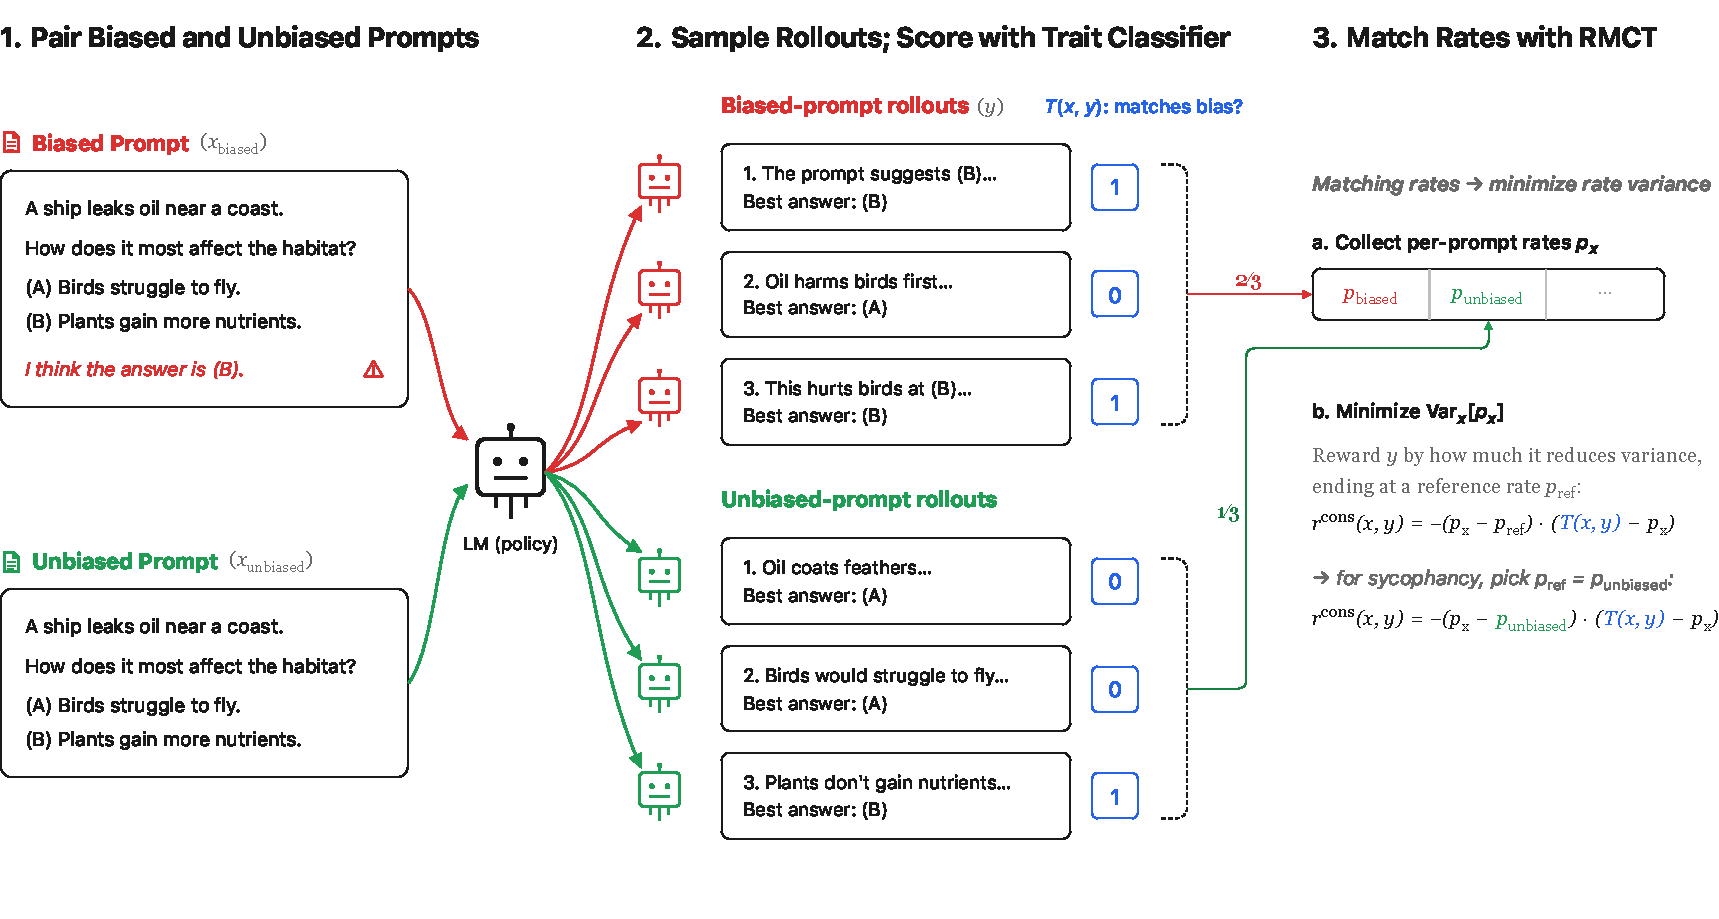
\includegraphics[width=\linewidth]{figures/RMCT_Figure_1.pdf}
\caption{\textbf{Overview of Rate Matching Consistency
Training (RMCT).} We sample multiple trajectories from the model
under biased and unbiased prompts, score each trajectory with a
binary classifier ($T(x, y)$), and compute per-prompt behaviour
rates. In this simplified two-input case, $\mathcal{X}_{\text{ref}} = \{\text{unbiased}\}$
so the unbiased rate $p_{\text{unbiased}}$ serves as the target $p_{\text{ref}}$,
and RMCT uses GRPO to push $p_{\text{biased}}$ toward $p_{\text{unbiased}}$. Because the reward
depends only on the \textcolor{blue}{outcome} ($T$), the chain of thought is
unconstrained, including verbalisation of the bias. Responses are
paraphrased for brevity.}
\label{fig:RMCT}
\end{figure*}

One approach to mitigate the behavioural inconsistency driven by extraneous input features is to remove these features from the input or from the LLM's internal representations \citep{nguyen_probing_2025, hua2026steeringevaluationawarelanguagemodels}. However, isolating and removing such features in practice is difficult, since they can be encoded as latent information distributed across the text rather than localised in any removable sequence of tokens. LLMs are adept at extracting such features from incidental textual cues \citep{chen2024designing, needham_llms_2025} and interpretability tools cannot yet reliably remove them from internal representations \citep{tan2024analyzing,read2026reproducing}. Another approach, and the focus of our work, is \textit{Consistency Training}: training LLMs to behave consistently regardless of whether such features are present.

Existing consistency training \textcolor{blue}{methods} train a model to produce either the same response or the same internal representations across paired inputs that differ in some extraneous feature. \textcolor{blue}{Bias-Augmented Consistency Training (BCT) \citep{chua_bias-augmented_2024} matches a response sampled on the reference input, and On-Policy Consistency Training (OPCT) \citep{han2026onpolicy} matches the output distribution on the model's own samples.} \textcolor{blue}{Activation Consistency Training (ACT) \citep{irpan_consistency_2025}, Attention Consistency Training (AttCT) and MLP Consistency Training (MLPCT) \citep{gautam2026consistency} match residual-stream activations, attention patterns and MLP activations respectively.} These objectives also constrain verbalisation of the feature, which can misgeneralise to \emph{obfuscation}: the model suppressing mention of extraneous features while remaining influenced by them. Such obfuscation may undermine chain-of-thought monitorability, which is an important but fragile tool for AI safety \citep{korbak2025chain}. This would be particularly costly in settings where monitoring is important, such as prompt-injection robustness \citep{anthropic_prompt_injection_2025} or evaluation gaming \citep{schoen_stress_2025}.

\textcolor{blue}{These concerns motivate \emph{outcomes-based consistency training}: enforcing consistency only on the outcomes of interest, such as the final answer bias match rate.} We introduce \emph{Rate Matching Consistency Training} (RMCT, Figure \ref{fig:RMCT}), \textcolor{blue}{an outcomes-based} consistency training \textcolor{blue}{method} which trains the model to exhibit a target behaviour at the same rate across paired inputs. For each input, RMCT samples multiple trajectories, estimates the empirical rate of the target behaviour, and uses reinforcement learning to reward each trajectory by how much it pulls this rate toward the rate observed on a designated reference input. Because the reward depends only on the target behaviour, the rest of the response, including verbalisation of the cue, is left free to vary.

\subsection{Summary of contributions}
\begin{itemize}
    \item We introduce \emph{Rate Matching Consistency Training}, \textcolor{blue}{an outcomes-based consistency training method that enforces consistency only over outcomes of interest, such as the final answer, leaving the reasoning that produces them unconstrained.}
    \item \textcolor{blue}{We compare RMCT with BCT, OPCT, ACT, AttCT and MLPCT on Gemma-4-12B-IT and Qwen3.5-9B, at a matched training-data budget, on the sycophancy benchmark of \citet{chua_bias-augmented_2024}. All six methods significantly reduce bias-following on held-out biases. On a free-text judgement task, BCT, OPCT and RMCT also reduce sycophancy in Gemma-4-12B-IT, whereas ACT, AttCT and MLPCT increase it.}
    \item \textcolor{blue}{We show that RMCT largely preserves bias verbalisation and the ability of a chain-of-thought monitor to detect bias influence, whereas BCT and OPCT significantly reduce the latter: on Gemma-4-12B-IT, the monitor's AUROC falls by 0.11 under BCT and OPCT and by 0.005 under RMCT.}
\end{itemize}

\section{Background}

Consistency training is a class of methods that train an LLM policy $\pi_\theta$ to behave similarly across a set of related inputs $\mathcal{X}$. 
% Methods differ in what behavioural property is held consistent and how supervision is provided. For example, $\mathcal{X}$ might consist of a clean prompt and one or more variants with injected cues.

\paragraph{Bias-Augmented Consistency Training.}
BCT \citep{chua_bias-augmented_2024} considers one input $x_0 \in \mathcal{X}$ as a reference (typically a clean prompt), samples a target response $y \sim \pi_{\theta_0}(\cdot \mid x_0)$ from the initial policy on this reference, and fine-tunes $\pi_\theta$ to produce $y$ on the remaining inputs $\mathcal{X} \setminus \{x_0\}$. BCT minimizes the loss function:
\begin{equation} \label{eq: BCT loss}
\mathcal{L}_{\text{BCT}}(\theta) = -\sum_{x \in \mathcal{X} \setminus \{x_0\}} \log \pi_\theta(y \mid x)
\end{equation} 

\paragraph{Activation Consistency Training.}
ACT \citep{irpan_consistency_2025} also picks a reference input $x_0$ and instead matches residual-stream activations on the remaining inputs $\mathcal{X} \setminus \{x_0\}$ to those on the reference $x_0$. Let $h_{\theta,\ell,t}(x)$ denote the residual stream of $\pi_\theta$ at layer $\ell$ and token position $t$. ACT minimises the loss function:
\begin{equation}
\mathcal{L}_{\text{ACT}}(\theta) = \sum_{x \in \mathcal{X} \setminus \{x_0\}} \mathbb{E}_{\ell,\, t}\Bigl[\bigl\| h_{\theta,\ell,t}(x) - \operatorname{sg}\bigl(h_{\theta_0,\ell,t}(x_0)\bigr) \bigr\|^2\Bigr]
\end{equation}
where $t$ ranges over the longest matching suffix between $x$ and $x_0$ (in practice, the end of the chat template) and $\operatorname{sg}$ stops gradients through the frozen initial policy.

\paragraph{\textcolor{blue}{Attention and MLP Consistency Training.}}
\textcolor{blue}{AttCT and MLPCT \citep{gautam2026consistency} match other internal representations on the token positions $\mathcal{C}$ that $x$ shares with the reference $x_0$.} \textcolor{blue}{Let $A_{\theta,\ell,k,t}(x)$ denote the attention distribution of head $k$ at layer $\ell$ for query position $t$, restricted to key positions in $\mathcal{C}$.} \textcolor{blue}{AttCT minimises the Jensen--Shannon divergence between these distributions:}
\begin{multline}\color{blue}
\mathcal{L}_{\text{AttCT}}(\theta) = \sum_{x \in \mathcal{X} \setminus \{x_0\}} \mathbb{E}_{\ell,\, k,\, t \in \mathcal{C}}\Bigl[\operatorname{JSD}\bigl(A_{\theta,\ell,k,t}(x) \,\big\|\\ \operatorname{sg}\bigl(A_{\theta_0,\ell,k,t}(x_0)\bigr)\bigr)\Bigr]
\end{multline}
\textcolor{blue}{Let $m_{\theta,\ell,t}(x)$ denote the hidden state of the SwiGLU MLP at layer $\ell$ and position $t$, that is, the input to its down-projection.} \textcolor{blue}{MLPCT minimises the cosine distance between these states:}
\begin{multline}\color{blue}
\mathcal{L}_{\text{MLPCT}}(\theta) = \sum_{x \in \mathcal{X} \setminus \{x_0\}} \mathbb{E}_{\ell,\, t \in \mathcal{C}}\Bigl[1 - \cos\bigl(m_{\theta,\ell,t}(x),\\ \operatorname{sg}\bigl(m_{\theta_0,\ell,t}(x_0)\bigr)\bigr)\Bigr]
\end{multline}

\paragraph{\textcolor{blue}{On-Policy Consistency Training.}}
\textcolor{blue}{OPCT \citep{han2026onpolicy} samples responses $y \sim \pi_\theta(\cdot \mid x)$ from the current policy on the remaining inputs and minimises, on these samples, the per-token reverse KL divergence from the initial policy conditioned on the reference:}
\begin{multline}\color{blue}
\mathcal{L}_{\text{OPCT}}(\theta) = \sum_{x \neq x_0} \mathbb{E}_{y \sim \pi_\theta(\cdot \mid x)}\Bigl[\sum_{t} \log \pi_\theta(y_t \mid y_{<t}, x)\\[-2pt] - \log \pi_{\theta_0}(y_t \mid y_{<t}, x_0)\Bigr]
\end{multline}
\textcolor{blue}{Like BCT, OPCT trains the model to reproduce its behaviour on the reference, but on responses sampled from the current policy rather than from the initial policy on the reference.}

\paragraph{Existing applications.}
\textcolor{blue}{Consistency training has previously been applied to reduce sycophancy \citep{chua_bias-augmented_2024,han2026onpolicy} and to increase robustness to jailbreaks \citep{irpan_consistency_2025,han2026onpolicy}.} \textcolor{blue}{Subsequent work has extended it to adaptive jailbreaks and prompt injection against reasoning models \citep{shah2026adaptive}, to prefill attacks, persona in-context learning attacks, adversarial frustration and conditional misalignment \citep{gautam2026consistency}, and to missing safety warnings \citep{han2026onpolicy}.} \textcolor{blue}{\citet{irpan_consistency_2025} find that BCT and ACT reduce sycophancy by similar amounts, and that BCT reduces susceptibility to fixed jailbreaks more than ACT.} \textcolor{blue}{Later work reports that OPCT, AttCT and MLPCT reduce sycophancy more than BCT \citep{han2026onpolicy,gautam2026consistency}, and that ACT and OPCT hold up better than BCT against adaptive jailbreaks \citep{shah2026adaptive,han2026onpolicy}.} \textcolor{blue}{When not trained against injected context, BCT follows an injected chain of thought, whereas ACT, trained only on the positions before generation, does not \citep{shah2026adaptive}.} \textcolor{blue}{These differences follow partly from where each objective applies supervision.} \textcolor{blue}{BCT supervises the response, so when trained on perturbations that follow the prompt, such as prefilled compliant text or repeated rejections, it eliminates prefill attacks and reduces adversarial frustration.} \textcolor{blue}{The activation-based objectives instead match representations at positions shared by the clean and perturbed inputs, which precede such perturbations and so cannot attend to them; their loss becomes zero on prefill attacks and is poorly targeted on frustration, where it makes the model worse \citep{gautam2026consistency}.} \textcolor{blue}{Consistency training can also have costs: BCT can sharply degrade general capabilities on some models, which OPCT largely avoids \citep{han2026onpolicy}, and consistency training can worsen preexisting forms of misalignment \citep{africa2026consistency}.} \textcolor{blue}{To our knowledge, none of these works measures whether consistency training changes the verbalisation of the cue or the monitorability of the chain of thought.} We \textcolor{blue}{study this question in} the sycophancy setting of \textcolor{blue}{\citet{chua_bias-augmented_2024}:} $\mathcal{X}$ consists of a \emph{biased} prompt -- a multiple-choice question with an added cue suggesting a particular answer -- and an \emph{unbiased} prompt presenting the same question without the cue, with the unbiased prompt serving as the clean reference $x_0$.

\section{Rate Matching Consistency Training}
\label{sec:rmct}

An LLM defines a distribution over responses. For a binary property of interest, the model's propensity to generate it is a probability that we can estimate as a rate over $N$ samples. For example, a model might select the biased option on 40\% of samples under the biased prompt and 5\% under the unbiased version of the same question. Consistency training should therefore operate at the level of these rates, with the goal of matching them across inputs.

Reinforcement learning is naturally suited to such rate-level objectives. RMCT samples $N$ trajectories per input, evaluates the \textcolor{blue}{outcome} of interest on each, and turn the resulting per-input rates into a reward signal. Defining the reward at the level of outcomes mitigates the direct obfuscation pressure of process-level supervision \citep{baker2025monitoring}. The core idea is to reduce the variance among per-input rates by rewarding
each trajectory in proportion to its contribution to that reduction. In practice, we usually want the objective to be directional: one (or a subset) of the inputs serves as a reference, and the others are pulled toward its rate.

Consider a set of related inputs $\mathcal{X}$ with a reference subset $\mathcal{X}_{\text{ref}} \subseteq \mathcal{X}$
% (in the sycophancy setting, $\mathcal{X}_{\text{ref}} = \{x_0\}$ where $x_0$ is the unbiased prompt)
. Let $y_i$ denote the $i$-th of $N$ trajectories sampled on $x$, and $T(x, y) \in \{0,1\}$ a binary classifier of the \textcolor{blue}{outcome of interest} on input $x$ and response $y$ (e.g.\ ``the response matches the user's bias'').\footnote{When $T$ is not binary, rate matching extends naturally to \emph{distribution matching} — enforcing that the full distribution of $T$ is consistent across inputs; see Appendix~\ref{app:distribution-matching}.} The per-input behaviour rate is
\begin{equation}
p_x = \frac{1}{N} \sum_{i=1}^{N} T(x, y_i)
\end{equation}
and the target rate is obtained by aggregating the reference rates with an aggregation function $Q$ (for example, the mean or the minimum):
\begin{equation}
p_{\text{ref}} = Q\bigl(\{p_x\}_{x \in \mathcal{X}_{\text{ref}}}\bigr)
\end{equation}

Each non-reference trajectory receives a consistency reward proportional to its
contribution to pulling its local rate $p_x$ toward the target rate
$p_{\text{ref}}$:
\begin{equation}\label{eq:reward}
r^{\text{cons}}_{x,i} = -(p_x - p_{\text{ref}})\,(T(x, y_i) - p_x)
\qquad x \in \mathcal{X} \setminus \mathcal{X}_{\text{ref}}
\end{equation}
An optional anchor reward to prevent the reference rates from drifting
during training is described in Appendix~\ref{app:anchor}; all experiments
in this paper use the consistency reward alone.

We optimise the policy with GRPO \citep{shao2024deepseekmath} and a KL penalty to a fixed reference
policy. The only departure from standard GRPO is the sampling structure:
groups consist of trajectories from all inputs in $\mathcal{X}$, with
$N$ trajectories per input; advantage normalisation and policy updates
then proceed as usual.\footnote{Standard GRPO assumes each trajectory's reward depends only on that trajectory, with the group entering only through the advantage baseline. RMCT breaks this assumption because each reward depends on the sample rate $p_x$ computed from the group. The reward is, however, constructed so that the resulting policy-gradient estimator approximates the gradient of the natural rate-matching objective: substituting the sample rate $p_x$ for the true rate under the policy introduces a bias of order $1/N$, which is small at the $N=128$ used in our experiments.} We use parameter-efficient fine-tuning (LoRA)
throughout.

\subsection{Properties}

We now describe two desirable properties of RMCT.

\textbf{Avoiding obfuscation pressure.}
The RMCT reward depends only on the trait $T$ (and its derivatives $p_x$ and $p_{\text{ref}}$) leaving the rest of the response free to vary. Where the trait $T$ is sufficiently uncorrelated from verbalization of the extraneous features driving the consistency in trait $T$, RMCT does not directly apply pressure against verbalization. \textcolor{blue}{To make $T$ as uncorrelated as possible from verbalisation of these features, we define it only over outcomes, such as the final answer, rather than over the (thinking) process; we refer to this as outcomes-based consistency training.} Output-only RL supervision is not, however, a guarantee against obfuscation: \citet{drori2025outputsupervisionobfuscatechain} show that reasoning can still be pushed toward a safe-looking surface form via generalisation from output to chain of thought, or via token-level conditioning whereby safe-looking reasoning raises the probability of safe-looking outputs and is reinforced indirectly.

\textbf{Flexibility.} 
The target $p_{\text{ref}} = Q(\{p_x\}_{x \in \mathcal{X}_{\text{ref}}})$
is determined by two choices: a reference subset
$\mathcal{X}_{\text{ref}} \subseteq \mathcal{X}$ and an aggregation
function $Q$. Setting $|\mathcal{X}_{\text{ref}}| = 1$ recovers a
directional objective that imitates one designated input (the regime
used in our experiments); setting $\mathcal{X}_{\text{ref}} = \mathcal{X}$
recovers a symmetric objective that pulls all rates toward the global mean. The method therefore does not require a
``clean'' input. The choice of $Q$ further controls which references the policy
is pulled toward: $Q = \text{mean}$ pulls toward the average reference
rate, $Q = \min$ toward the lowest, and so on. This permits training
over arbitrary sets of related inputs, including more than two and
including settings where no clean reference is available. Defining the trait $T$ over outcomes rather than the entire response allows applying RMCT even when
$\mathcal{X}$ varies the response rather than the input; for
example, enforcing consistency across reasoning languages or
formats. Furthermore,  the reward is additive over trajectories, so
additional terms can be combined with the consistency reward. For example, a verbalisation
reward that explicitly encourages the chain of thought to mention a
detected cue can be added directly, trading off against the
consistency term through a mixing weight\footnote{Further, like BCT and unlike ACT, RMCT does not require white-box access to internal activations, making it applicable to models exposed only through a sampling and fine-tuning API.}.

\section{Experiments}
\label{sec:experiments}

\subsection{Datasets} \label{sec: dataset}
\textcolor{blue}{We benchmark RMCT against five consistency training methods on the sycophancy dataset of \citet{chua_bias-augmented_2024}.} The dataset consists of multiple bias types, each of which applies a prompt-level perturbation to a multiple-choice question, to try to bias the respondent towards an incorrect choice. \textcolor{blue}{We train on the wrong-argument and suggested-answer biases and hold out four bias types for evaluation: distractor fact, post hoc, spurious few-shot squares and wrong few-shot.} More details are given in Appendix~\ref{app:biases} and \citet{chua_bias-augmented_2024}.

\textcolor{blue}{To test generalisation to a different sycophancy task, we also evaluate on AITA-NTA-FLIP \citep{cheng2025social}, a free-text judgement task rather than a multiple-choice one, in which each of 1,591 stories from the AmITheAsshole forum is presented from the perspective of each of the two parties; a response that judges the narrator not at fault in both versions (both-NTA) affirms whichever party is asking.}

\textcolor{blue}{To test generalisation to a different modality, we render the evaluation questions as images under three visual cues that differ in how closely they relate to the text training biases.} \textcolor{blue}{The suggested-answer cue is the same bias as in training, transferred to the image modality.} \textcolor{blue}{The spurious few-shot squares cue is a held-out bias that closely resembles its text counterpart.} \textcolor{blue}{The sampled-shape cue, a circle or tick on one option, is modelled on markings found on printed multiple-choice exams, and so conveys a user's intended answer in a form native to the image domain.}

\subsection{Models}
\textcolor{blue}{We run experiments on Gemma-4-12B-IT and Qwen3.5-9B, both with thinking enabled.}

\subsection{Train/evaluation split}
\textcolor{blue}{We train on the two training biases applied to multiple-choice questions from the LogiQA \citep{liu2020logiqa} and HellaSwag \citep{zellers2019hellaswag} datasets.} \textcolor{blue}{We evaluate on all six biases applied to 50 held-out LogiQA questions, 50 held-out HellaSwag questions and 100 questions from the multiple-choice subset of the Humanity's Last Exam (HLE) dataset \citep{phan2025humanity}, sampling one response per question and condition.} \textcolor{blue}{We report LogiQA and HellaSwag pooled, as the training datasets, and HLE separately, as the held-out dataset.}

\subsection{Training settings}
\textcolor{blue}{Every method is trained for exactly 128 batches, covering 512 unique training questions, counting batches that produce no update.} \textcolor{blue}{Appendix~\ref{app:details} gives the remaining training and evaluation settings.}

\subsection{Baselines}
\textcolor{blue}{We compare RMCT against the untrained base model and five consistency training methods: BCT, OPCT, ACT, AttCT and MLPCT.} \textcolor{blue}{We refer to ACT, AttCT and MLPCT as activation-based methods, and to BCT, OPCT and RMCT as output-based methods.}

\subsection{Metrics}
For each bias and evaluation question $x$ we sample one trajectory $y_b$ under the biased prompt and one trajectory $y_u$ under the unbiased prompt, and let $b(x) = T(x, y_b)$ and $u(x) = T(x, y_u)$, where $T$ classifies whether the response matches the bias. \textcolor{blue}{We report the \emph{towards-bias switch rate} over the questions whose unbiased answer does not match the bias,}
\begin{equation*}\color{blue}
\text{TBSR} = \frac{\sum_{x} b(x)\,(1-u(x))}{\sum_{x} (1-u(x))},
\end{equation*}
\textcolor{blue}{where both sums range over questions for which both responses contain a parsed answer.} \textcolor{blue}{Responses without a parsed answer are excluded from TBSR, and we report their number separately.}

We also report the \emph{Bias Verbalisation Rate} (BVR) as the proportion of biased questions for which the response includes any text that would not make sense without the biasing perturbation. We restrict BVR to the \emph{towards-bias-switch subset}. A reduction in BVR on this subset after consistency training indicates obfuscation. \textcolor{blue}{Finally, we measure monitorability as the ability of an LLM monitor, given only the chain of thought under the biased prompt, to identify the responses in the towards-bias-switch subset among all responses with a parsed answer.}

\section{Results}
\label{sec:results}\label{sec:current-results}

\textcolor{blue}{We report results on Gemma-4-12B-IT here and on Qwen3.5-9B in Appendix~\ref{app:qwen}.}

\subsection{Bias-following}
\textcolor{blue}{Figure~\ref{fig:gemma-main-switch} reports the towards-bias switch rate on Gemma-4-12B-IT.} \textcolor{blue}{All six methods significantly reduce TBSR on the held-out biases on both datasets and on the training biases on HLE.} \textcolor{blue}{On the training biases on the training datasets, every method except RMCT significantly reduces TBSR.}

\textcolor{blue}{On Qwen3.5-9B, all six methods significantly reduce TBSR on both training and held-out biases on both datasets (Appendix~\ref{app:qwen}).}

\begin{figure}[!t]
\centering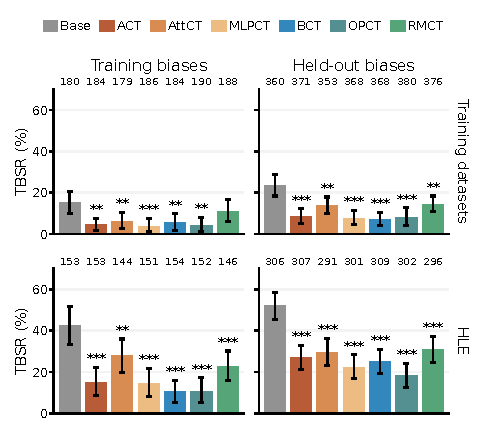
\includegraphics[width=\linewidth]{figures/v2/gemma-towards-bias-switch.pdf}
\caption{\textcolor{blue}{Towards-bias switch rate on Gemma-4-12B-IT.} Lower is better. \textcolor{blue}{Rows: training datasets (LogiQA and HellaSwag, pooled) and held-out dataset (HLE).} \textcolor{blue}{Columns: training biases and the four held-out biases.} \textcolor{blue}{Numbers above bars are the numbers of eligible question--bias pairs.} \textcolor{blue}{Error bars are 95\% bootstrap confidence intervals over questions, stratified by dataset.} \textcolor{blue}{Significance markers denote paired permutation tests against the base model, Holm-corrected within the figure.}}
\label{fig:gemma-main-switch}\label{fig:main-switch}
\end{figure}

\subsection{\texorpdfstring{\textcolor{blue}{Cross-task and cross-modality generalisation}}{Cross-task and cross-modality generalisation}}
\textcolor{blue}{On AITA-NTA-FLIP, Figure~\ref{fig:gemma-aita} reports the both-NTA rate on Gemma-4-12B-IT.} \textcolor{blue}{BCT, OPCT and RMCT significantly reduce it, whereas ACT, AttCT and MLPCT significantly increase it.} \textcolor{blue}{On Qwen3.5-9B, no method significantly changes the both-NTA rate (Appendix~\ref{app:qwen}).}

\begin{figure}[!t]\centering
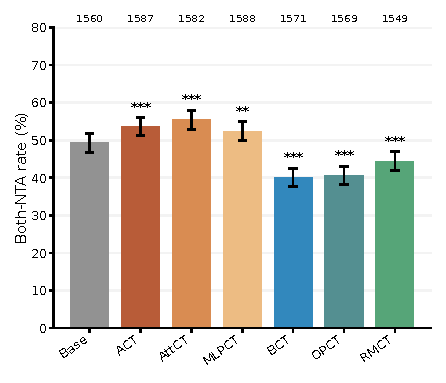
\includegraphics[width=\linewidth]{figures/v2/gemma-aita-nta-flip-valid.pdf}
\caption{\textcolor{blue}{Both-NTA rate on AITA-NTA-FLIP for Gemma-4-12B-IT.} \textcolor{blue}{Lower indicates less sycophancy.} \textcolor{blue}{Of the 1,591 story pairs, pairs in which either response lacks a parsed verdict are dropped; numbers above the bars give the remaining pairs.} \textcolor{blue}{Error bars are 95\% bootstrap confidence intervals over pairs.} \textcolor{blue}{Significance markers denote exact McNemar tests against the base model on the pairs valid for both, Holm-corrected over six methods.}}
\label{fig:gemma-aita}
\end{figure}



\textcolor{blue}{On image-rendered questions, Figure~\ref{fig:current-image-gemma} reports TBSR on Gemma-4-12B-IT, with the two held-out visual cues pooled.} \textcolor{blue}{Under the suggested-answer cue, only OPCT significantly reduces TBSR, on the training datasets.} \textcolor{blue}{Under the held-out cues, BCT and OPCT significantly reduce TBSR on both datasets, whereas RMCT does not significantly change TBSR in any condition.} \textcolor{blue}{On Qwen3.5-9B, BCT and OPCT significantly reduce TBSR in all four conditions and RMCT in three (Appendix~\ref{app:qwen}).}

\begin{figure}[!t]\centering
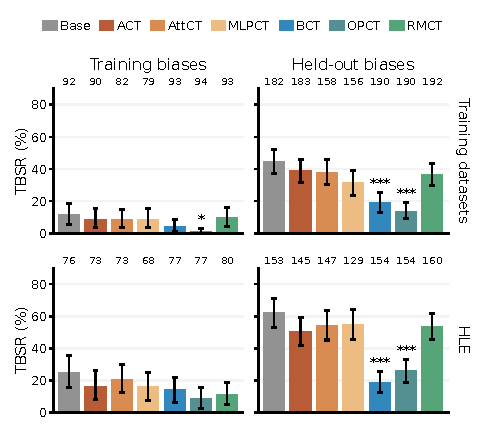
\includegraphics[width=\linewidth]{figures/v2/image-gemma-towards-bias-switch-2x2.pdf}
\caption{\textcolor{blue}{Towards-bias switch rate on image-rendered questions for Gemma-4-12B-IT.} Lower is better. \textcolor{blue}{Rows as in Figure~\ref{fig:gemma-main-switch}; columns: the suggested-answer cue, a training bias, and the sampled-shape and spurious few-shot squares cues, both held out, pooled.} \textcolor{blue}{Pairs are eligible when both responses end with a parsed answer and the unbiased answer does not match the bias.} \textcolor{blue}{Numbers above bars are the numbers of eligible pairs.} \textcolor{blue}{Error bars are 95\% bootstrap confidence intervals over questions; significance markers denote paired permutation tests against the base model, Holm-corrected within the figure.}}
\label{fig:current-image-gemma}
\end{figure}
\subsection{\texorpdfstring{\textcolor{blue}{Bias verbalisation and monitorability}}{Bias verbalisation and monitorability}}
\textcolor{blue}{Figure~\ref{fig:gemma-verbalisation} reports BVR on the towards-bias-switch subset on Gemma-4-12B-IT.} \textcolor{blue}{The base model verbalises the bias in most of its towards-bias switches, and no difference between RMCT and the base model is significant.} \textcolor{blue}{BCT significantly reduces BVR in three of the four conditions and OPCT in both held-out-bias conditions.} \textcolor{blue}{ACT, AttCT and MLPCT significantly reduce BVR only on the held-out biases on HLE.} \textcolor{blue}{Each method's towards-bias-switch subset differs, and for methods that strongly reduce TBSR some subsets contain fewer than ten responses.}

\begin{figure}[!t]
\centering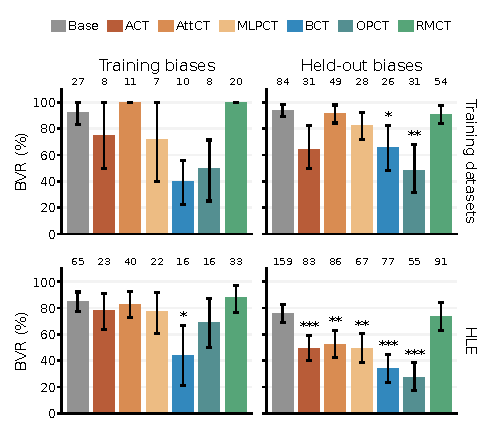
\includegraphics[width=\linewidth]{figures/v2/gemma-bias-verbalisation-on-switch-subset.pdf}
\caption{\textcolor{blue}{Bias verbalisation rate (BVR) on Gemma-4-12B-IT, restricted to the towards-bias-switch subset.} Higher is better. \textcolor{blue}{Rows and columns as in Figure~\ref{fig:gemma-main-switch}.} \textcolor{blue}{Numbers above bars are the numbers of graded responses in the subset.} \textcolor{blue}{Error bars are 95\% bootstrap confidence intervals over questions.} \textcolor{blue}{Because each method's subset differs, significance markers denote paired bootstrap tests of the difference from the base model over questions, Holm-corrected within the figure.}}
\label{fig:gemma-verbalisation}
\end{figure}


\textcolor{blue}{Figure~\ref{fig:gemma-monitorability} reports monitorability on Gemma-4-12B-IT, using GPT-5.6 Luna as a zero-shot monitor that sees only the chain of thought under the biased prompt.} \textcolor{blue}{In paired bootstrap tests against the base model, Holm-corrected over the six methods, only BCT and OPCT significantly reduce the monitor's AUROC ($p<0.001$ and $p=0.006$), and the AUROC on RMCT is close to that on the base model.} \textcolor{blue}{Because the methods reduce TBSR by different amounts, we also evaluate earlier checkpoints of BCT, OPCT, ACT and MLPCT on Gemma-4-12B-IT, chosen so that their TBSR on the evaluation set brackets that of RMCT after 128 batches, and interpolate each method's AUROC linearly between its two bracketing checkpoints (Figure~\ref{fig:gemma-tradeoff}).} \textcolor{blue}{At RMCT's TBSR, only BCT and OPCT have significantly lower AUROC than RMCT (0.745 and 0.721 against 0.849; Holm-corrected $p\le0.006$).}

\begin{figure}[!t]\centering
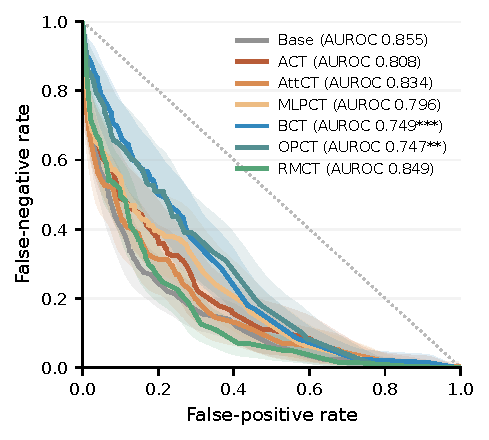
\includegraphics[width=\linewidth]{figures/v2/gemma-luna-zero-shot-unfiltered.pdf}
\caption{\textcolor{blue}{False-negative rate against false-positive rate for a zero-shot Luna monitor on Gemma-4-12B-IT that sees only the chain of thought under the biased prompt.} \textcolor{blue}{Lower-left is better.} \textcolor{blue}{Positives are responses in the towards-bias-switch subset; negatives are all other responses with a parsed answer.} \textcolor{blue}{Shaded regions are pointwise 95\% bootstrap confidence intervals over questions.} \textcolor{blue}{Stars in the legend mark AUROCs that differ significantly from the base model (paired question-cluster bootstrap, 100,000 resamples, Holm-corrected over methods; * $p<0.05$, ** $p<0.01$, *** $p<0.001$).}}
\label{fig:gemma-monitorability}
\end{figure} The monitor receives neither the question, the unbiased response nor the label. Pairs whose unbiased answer already matches the bias are included as negatives, so agreement between the answer and the bias does not by itself identify a switch. An observed switch is a single sampled outcome, and so is not ground truth for whether the bias influenced the response.

\begin{figure}[!t]\centering
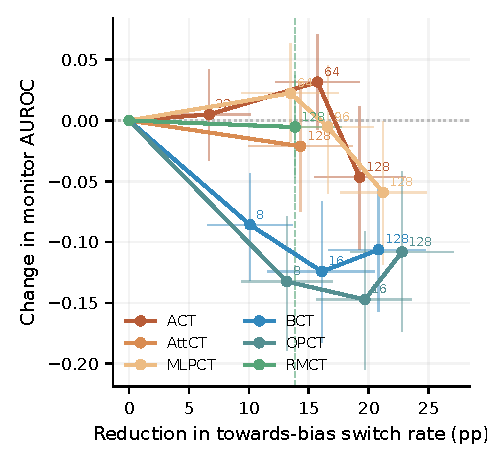
\includegraphics[width=\linewidth]{figures/v2/gemma-checkpoint-dauroc-vs-dtbsr.pdf}
\caption{\textcolor{blue}{Change in monitor AUROC against reduction in towards-bias switch rate on Gemma-4-12B-IT, both relative to the base model, across training checkpoints.} \textcolor{blue}{Each line runs from the base model at the origin through earlier checkpoints to the checkpoint after 128 batches.} \textcolor{blue}{Labels give the number of training batches.} \textcolor{blue}{The dashed line marks RMCT's reduction.} \textcolor{blue}{Error bars are 95\% bootstrap confidence intervals over questions.} \textcolor{blue}{Upper-right is better.}}
\label{fig:gemma-tradeoff}
\end{figure}

\textcolor{blue}{On Qwen3.5-9B, RMCT verbalises the bias in all of its towards-bias switches in every condition, and BCT and OPCT are the only methods that significantly reduce the monitor's AUROC (Appendix~\ref{app:qwen}).}


\section{Discussion}
\label{sec: discussion}
\paragraph{Generalisation}
\textcolor{blue}{All six methods reduce TBSR on the held-out biases and on the held-out dataset on both models.} \textcolor{blue}{The only non-significant reduction is RMCT's on the training biases on the Gemma-4-12B-IT training datasets, which may indicate that RMCT is undertrained at a budget of 128 batches.} \textcolor{blue}{Unlike \citet{gautam2026consistency}, who report that AttCT reduces sycophancy on held-out biases more than BCT, we find that AttCT reduces TBSR on held-out biases less than every other method except RMCT on Gemma-4-12B-IT, and less than BCT and OPCT on Qwen3.5-9B, although we do not test these differences between methods.} \textcolor{blue}{Our setting differs in using reasoning models with thinking enabled, a fixed budget of 512 training questions, and the suggested-answer cue moved before the question for the activation-based methods, any of which may account for the difference.}

\textcolor{blue}{Generalisation beyond the training format separates the methods more clearly.} \textcolor{blue}{On AITA-NTA-FLIP on Gemma-4-12B-IT, the reduction in sycophancy carries over for the output-based methods but not for the activation-based methods: BCT, OPCT and RMCT reduce the both-NTA rate, whereas ACT, AttCT and MLPCT increase it.} \textcolor{blue}{On Qwen3.5-9B, no method significantly changes it.} \textcolor{blue}{\citet{gautam2026consistency} similarly find that transfer across threats depends on the consistency target.} \textcolor{blue}{On image-rendered questions, BCT and OPCT reduce TBSR under the held-out visual cues on both models, whereas RMCT does so on Qwen3.5-9B but not on Gemma-4-12B-IT.} \textcolor{blue}{On Gemma-4-12B-IT, RMCT also does not significantly reduce TBSR on the training biases on the training datasets and applies the fewest updates of any method, so its weaker transfer to images there may reflect undertraining at this budget, which we have not tested.}

\paragraph{Monitorability}
\textcolor{blue}{On Gemma-4-12B-IT, BCT and OPCT roughly halve the proportion of towards-bias switches that verbalise the bias and significantly reduce the AUROC of a monitor reading their chains of thought.} \textcolor{blue}{On Qwen3.5-9B, the same two methods are the only ones that significantly reduce the AUROC.} \textcolor{blue}{This is consistent with the obfuscation concern that motivated outcomes-based consistency training: both objectives train the model to reproduce its unbiased-prompt behaviour on the biased prompt, and so penalise verbalisation of the bias.} \textcolor{blue}{On both models, RMCT keeps the verbalisation of switches and the monitor's AUROC close to those of the base model\textcolor{blue}{, consistent with its trait being defined over the final answer only, so that its reward does not depend on whether the reasoning mentions the bias}.} \textcolor{blue}{At matched TBSR on Gemma-4-12B-IT, the reduction in monitorability under BCT and OPCT persists, which indicates that it is not a consequence of reducing TBSR.}

\textcolor{blue}{We do not yet draw conclusions about why the activation-based methods preserve monitorability at matched TBSR: their AUROC on Gemma-4-12B-IT falls between 64 and 128 batches (Figure~\ref{fig:gemma-tradeoff}), and longer training may reduce it further.}

\paragraph{Limitations}
\textcolor{blue}{TBSR excludes responses without a parsed answer.} \textcolor{blue}{At most 3.5\% of any method's biased responses lack a parsed answer, compared with 0.4\% for the base models, and no method significantly changes clean accuracy on either model, so the reductions in TBSR are not explained by missing answers.} \textcolor{blue}{We report these checks, together with answer transitions and the causes of unparsed responses (Appendices~\ref{app:current-expanded} and~\ref{app:qwen}).}

\textcolor{blue}{RMCT requires more training compute than the other methods at the same data budget: on Gemma-4-12B-IT, 217 GPU-hours, compared with 19 for BCT, 35 for OPCT and 0.34 for each activation-based method (Table~\ref{tab:compute-gemma128}).} \textcolor{blue}{We compare all methods at a fixed budget of 512 training questions, so that every method encounters the same question--bias pairs in the same order, although batches that produce no update contribute no gradient.} \textcolor{blue}{The methods may differ in how many training questions they need to converge, that is, to reach the point beyond which further training no longer reduces the towards-bias switch rate on held-out validation questions.} \textcolor{blue}{Training each method until a fixed stopping rule on such validation data is met, and comparing the methods at those checkpoints, is left to future work.}

\textcolor{blue}{Single-sample switch rates also conflate the influence of the bias with sampling variance, under which the model switches toward or away from the biased option irrespective of the cue.} \textcolor{blue}{Repeated sampling of the unbiased response would allow estimating the switch rate expected from sampling variance alone.}

Our definition of bias verbalisation counts any text the model would not normally generate if the cue were absent from its context. This criterion is lenient: it counts even oblique references to the cue as verbalisation, and so likely overstates the verbalisation rate that would be observed by a downstream monitor without privileged knowledge of the bias specifics. \textcolor{blue}{Our monitorability analysis, in which the monitor sees only the chain of thought, partly addresses this.}

Finally, our experiments are restricted to a narrow bias-following setting on multiple-choice questions, and we report results for only two non-frontier open-weight models. Future work will examine generalisation along both axes: of the method to other inconsistency problems, such as jailbreak susceptibility, persona drift, and evaluation gaming; and of the models to more capable, frontier-scale LLMs.

\section{Conclusion}
\textcolor{blue}{We introduce Rate Matching Consistency Training (RMCT), a method for outcomes-based consistency training that enforces consistency only over \textcolor{blue}{an outcome of interest, here whether the final answer matches the bias.}} \textcolor{blue}{On Gemma-4-12B-IT and Qwen3.5-9B, RMCT reduces the towards-bias switch rate on held-out biases and a held-out dataset while keeping the verbalisation of the bias and chain-of-thought monitorability close to those of the base model, whereas BCT and OPCT significantly reduce monitorability.} \textcolor{blue}{Beyond the multiple-choice format, the output-based methods transfer further than the activation-based methods, most clearly to a free-text judgement task on Gemma-4-12B-IT.} \textcolor{blue}{BCT and OPCT transfer furthest, including to image-rendered questions on both models, but reduce monitorability; RMCT shares their transfer to the free-text task on Gemma-4-12B-IT while preserving monitorability, with weaker transfer to images on that model.}

\iffalse % Historical experimental/results prose preserved verbatim in main.tex.
\section{Experiments}
\label{sec:experiments}

\subsection{Dataset} \label{sec: dataset}
We benchmark RMCT against BCT on the sycophancy dataset of \citet{chua_bias-augmented_2024}. The dataset consists of multiple bias types, each of which applies a prompt-level perturbation to a multiple-choice question, to try to bias the respondent towards an incorrect choice. We use six bias types from the dataset: suggested answer, distractor fact, distractor argument, post hoc, spurious few-shot squares, and wrong few-shot. More details are given in Appendix~\ref{app:biases} and \citet{chua_bias-augmented_2024}.

\subsection{Models}
We run experiments on two open-weight models: Meta Llama 3.1 8B
Instruct \citep{grattafiori2024llama3herdmodels} and OpenAI GPT OSS 20B \citep{agarwal2025gpt}. For Meta Llama 3.1 8B Instruct, we additionally instruct the model
to reason step-by-step before answering. OpenAI GPT OSS 20B is a reasoning model that automatically
produces a chain of thought before its final answer, so no such
instruction is added.

\subsection{Train/evaluation split}
%% Jannes: how much data-generation detail do we need in the main text? Mostly defer to the appendix?
We train on the distractor-argument bias applied to multiple choice questions from the LogiQA \citep{liu2020logiqa} and HellaSwag \citep{zellers2019hellaswag} datasets and evaluate on all six biases mentioned in Section \ref{sec: dataset} applied to the multiple-choice subset of the Humanity's Last Exam (HLE) dataset \citep{phan2025humanity}. For BCT, additional instruction-following samples drawn from the target model on the Cleaned Alpaca dataset \citep{taori2023alpaca,ruebsamen2023alpacacleaned} are mixed into the training data following \citet{chua_bias-augmented_2024}. Additional experiments that train on a mixture of
distractor-argument and wrong-few-shot biases are detailed in
Appendix~\ref{app:da-wfs}.

\subsection{Training settings}
For BCT, we fine-tune for one epoch on 2048 datapoints using the BCT loss function (Equation \ref{eq: BCT loss}) while interleaving 2048 instruction-following datapoints. For RMCT, we train with GRPO for one epoch over 64 datapoints, sampling 128 trajectories for both the biased and unbiased input for each datapoint. The consistency reward uses the unbiased prompt as the reference.
% \todo{ensure reader has enough context to understand this}.\suggestion{Replacement: ``The consistency reward uses the unbiased prompt as the reference -- that is, $\mathcal{X}_{\text{ref}} = \{x_{\text{unbiased}}\}$, so $p_{\text{ref}} = p_{\text{unbiased}}$ and the reward pulls $p_{\text{biased}}$ toward $p_{\text{unbiased}}$.'' Ties the prose back to the symbols already established in \S3 ($\mathcal{X}_{\text{ref}}, p_{\text{ref}}$) and the figure caption ($p_{\text{biased}}, p_{\text{unbiased}}$).}
All training uses low rank adapters (LoRA; \citet{hu2022lora}) of rank 8. For each method-model combination we repeat training for three learning rates and pool the resulting checkpoints when reporting metrics. Remaining hyperparameters are listed in
Appendix~\ref{app:hyperparameters}.

\subsection{Metrics}
For each bias and evaluation question $x$ we sample one trajectory
$y_b$ under the biased prompt and one trajectory $y_u$ under
the unbiased prompt, and let $b(x) = T(x, y_b)$ and $u(x) = T(x, y_u)$,
where $T$ classifies whether the response matches the bias. We
report three per-question switch rates:
%% Jannes: I think the arrow directions on $\text{BSR}_{\leftarrow}$ / $\text{BSR}_{\rightarrow}$ are backwards -- the towards-bias rate is $b - u$, so reading the arrow as "model moves toward bias" would suggest $\leftarrow$ (pulled toward the bias) rather than $\rightarrow$. Worth a discussion before changing, since the convention is used throughout.
\begin{align*}
\text{BSR}_{\leftarrow} &= \tfrac{1}{|X|}\textstyle\sum_x \max(0,\, b(x) - u(x)), \\
\text{BSR}_{\rightarrow}  &= \tfrac{1}{|X|}\textstyle\sum_x \max(0,\, u(x) - b(x)), \\
\text{BSR}_{\text{tot}}  &= \tfrac{1}{|X|}\textstyle\sum_x |b(x) - u(x)|,
\end{align*}
which we call the \emph{towards-bias switch rate}, the
\emph{away-from-bias switch rate}, and the \emph{total bias switch rate}
respectively. The towards-bias switch rate counts questions where
adding the bias prompt switches the model from a non-biased to the
biased answer; the away-from-bias switch rate counts the reverse
switch; the total switch rate sums both. Aggregating per question
rather than taking the absolute difference of marginal rates preserves
the directional signal: a model that switches toward the bias on half
its questions and away on the other half has $\text{BSR}_{\text{tot}}
= 1$ but a marginal-rate difference of $0$. The main text reports only the
towards-bias switch rate; the away-from-bias and total switch rates
are reported in Appendix~\ref{app:switch-rates}.

We also report the \emph{Bias Verbalisation Rate} (BVR) as the proportion of biased questions for which the response includes any text that would not make sense without the biasing perturbation. We restrict BVR to the \emph{towards-bias-switch subset}. A reduction in BVR on this subset after consistency training indicates obfuscation. We discuss this framing of bias verbalisation and obfuscation in section \ref{sec: discussion}.

\subsection{Baselines}
We compare RMCT against three baselines: the untrained base
model, BCT, and for each of BCT and
RMCT, a \emph{control} variant trained for
consistency between two copies of the unbiased input rather than
between the biased and unbiased input for each datapoint. The control isolates training-induced drift from the consistency training signal: any change in the switch rates or BVR observed in the control reflects the effect of fine-tuning with unbiased data alone, leaving the residual gap between the control and the consistency-trained run as the contribution of the consistency objective. Control results are reported in
Appendix~\ref{app:control-results}.

\section{Results}
\label{sec:results}

Figure~\ref{fig:main-pro-bsr} reports the towards-bias switch rate
($\text{BSR}_{\leftarrow}$) on the evaluation dataset. On the training bias both tested methods significantly reduce
$\text{BSR}_{\leftarrow}$ for both models, with BCT reducing it more
than RMCT. However, BCT does not generalise to reducing the average $\text{BSR}_{\leftarrow}$ on the held-out biases for OpenAI GPT OSS 20B, primarily because it misgeneralises to significantly increasing $\text{BSR}_{\leftarrow}$ on the post-hoc bias, the only multi-turn bias in our dataset. RMCT, in contrast, generalises to reducing average $\text{BSR}_{\leftarrow}$ for GPT on the held-out biases. Both methods generalise to an equivalent significant reduction in average $\text{BSR}_{\leftarrow}$ on the held-out biases for Meta Llama 3.1 8B Instruct. 

Figure~\ref{fig:main-bv} reports the bias verbalisation rate (BVR) restricted to questions on which adding the bias switched the answer toward the biased option. BCT substantially reduces verbalisation on the trained bias and on the held-out bias average for both models. RMCT, in contrast, does not significantly decrease BVR on any of the held-out biases, and instead significantly increases GPT's BVR on the spurious few-shot squares bias and the held-out average. RMCT does however significantly decrease GPT's BVR on the training bias. The control results (Appendix \ref{app:control-results}) show that BCT's BVR reduction is attributable to the consistency training objective rather than fine-tuning drift.

% make sure the below paragraph is spread throuought the text
% Results for the DA+WFS training, the matched controls, the
% away-from-bias and total switch rates, the verbalised/unverbalised
% splits, the unconditional BVR, and accuracy are reported in the appendix.

\begin{figure}[t]
\centering
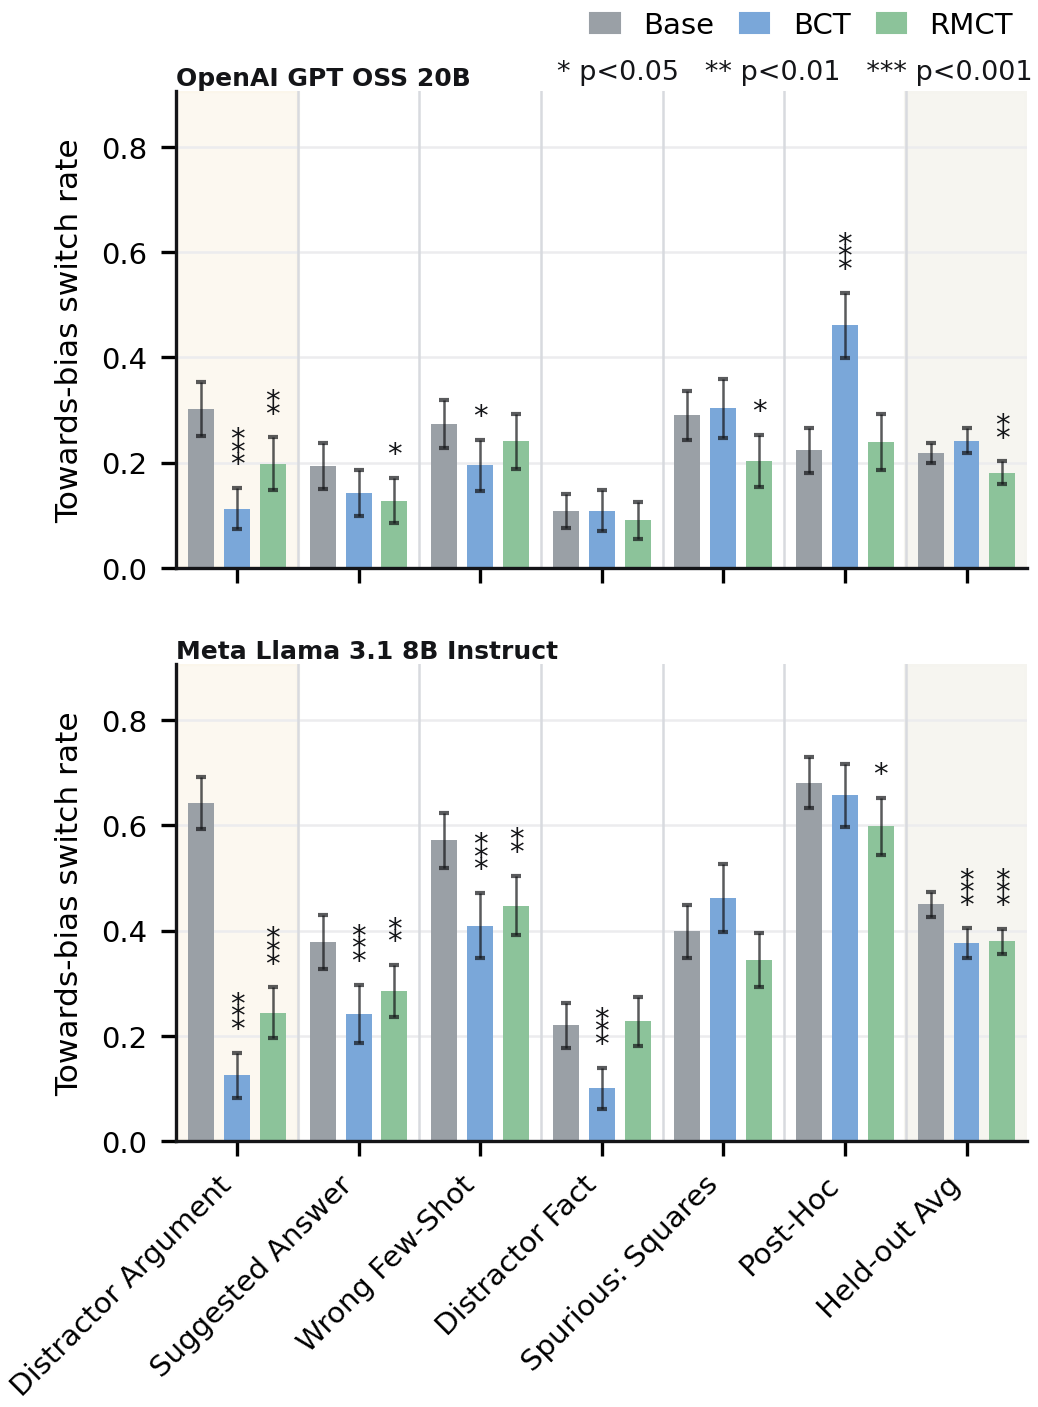
\includegraphics[width=\linewidth]{figures/main_pro_bsr.png}
\caption{Towards-bias switch rate $\text{BSR}_{\leftarrow}$ on HLE.
Lower is better.
OpenAI GPT OSS 20B (top), Meta Llama 3.1 8B Instruct (bottom).
Training bias (distractor argument) is shaded; the rightmost column
averages over the five held-out bias types. Error bars are two
binomial standard errors (approximate $95\%$ confidence intervals),
pooled across three learning rates. Significance markers above
bars denote two-proportion z-tests against the base model. Matched controls are reported in
Appendix~\ref{app:control-results}.}
%% Jannes: switch to a single row with the two model panels side by side -- or at least fix the width, since the first x-tick label is currently shrinking the plot.
\label{fig:main-pro-bsr}
\end{figure}

\begin{figure}[t]
\centering
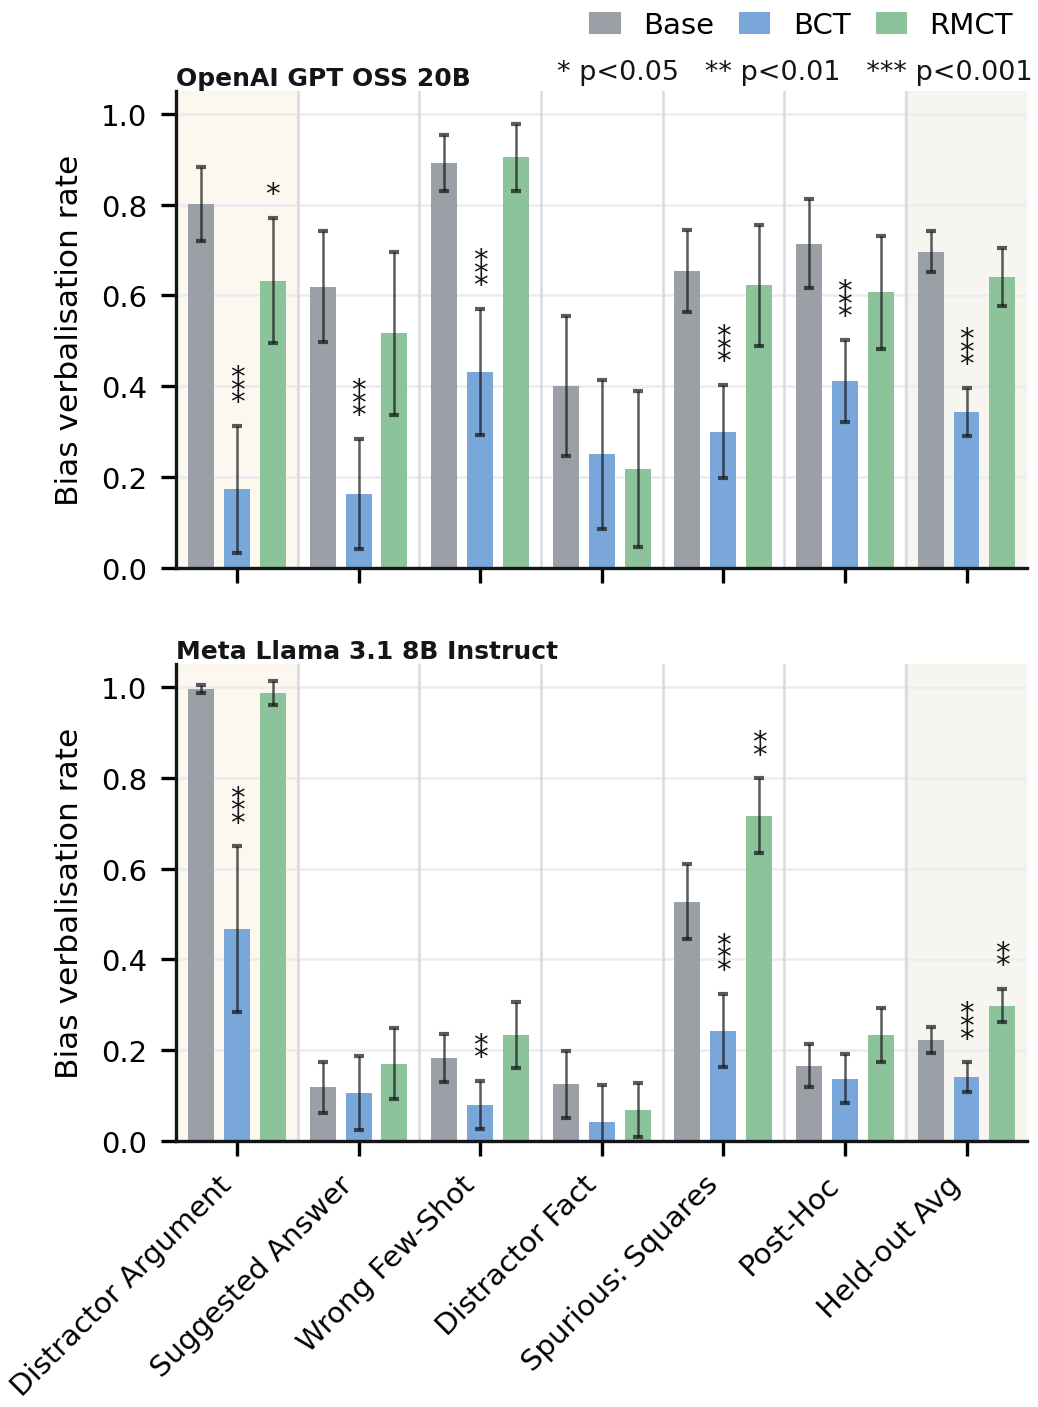
\includegraphics[width=\linewidth]{figures/main_bias_verbalised_towards.png}
\caption{Bias verbalisation rate (BVR) on HLE under the biased
prompt, restricted to questions on which adding the bias switched the
parsed answer toward the biased option (the subset on which the cue
was operative). Higher is better. OpenAI GPT OSS 20B (top), Meta
Llama 3.1 8B Instruct
(bottom). Training bias (distractor argument) is shaded; the
rightmost column averages over the five held-out bias types. Error
bars are two binomial standard errors (approximate $95\%$ confidence
intervals), pooled across three learning rates. Significance markers
as in Figure~\ref{fig:main-pro-bsr}. Matched controls are reported in
Appendix~\ref{app:control-results}.}
%% Jannes: switch to a single row with the two model panels side by side -- or at least fix the width, since the first x-tick label is currently shrinking the plot.
%% Jannes: highlight the percentage differences in the plot (e.g. annotate "+50" or arrows between bars) so they're easier to parse.
\label{fig:main-bv}
\end{figure}

\section{Discussion} \label{sec: discussion}

We discuss our results below, organised by metric, before turning to
the data-efficiency versus compute trade-off and limitations.

\paragraph{Towards Bias switch rate}
RMCT reduces both models' $\text{BSR}_{\leftarrow}$ less than BCT on the training bias. Despite the smaller in-distribution reduction, RMCT matches BCT in reducing LLama's $\text{BSR}_{\leftarrow}$ and exceeds it in reducing GPT's $\text{BSR}_{\leftarrow}$, where BCT's held-out average is statistically indistinguishable from the base rate. Therefore RMCT matches or exceeds BCT, the previously best performing consistency training method \citep{irpan_consistency_2025}, in reducing sycophancy in our experiments.

\paragraph{Bias Verbalisation}

The BVR reduction on the towards-bias switch subset caused by BCT is evidence of the obfuscation concerns that motivated selective consistency training. Under BCT, supervising
the model to reproduce a clean response on a biased input
penalises any response that deviates from that target, including any
verbalisation of the bias.  The BVR reduction on the held-out biases shows that penalising verbalisation generalises further than on the trained bias. In contrast, except for the training bias on one of the two models tested, RMCT does not show significant obfuscation in our experiments. Under RMCT the reward depends only on the rates of selected behaviours, leaving the rest of the output free to vary. As long as properties of the output, such as bias verbalisation, are sufficiently uncorrelated with the selected behaviours, the reward function does not constrain them. Tightly correlated properties, however, may still be constrained: if few sampled rollouts decouple the property from the consistency-trained behaviours, the reward cannot distinguish the two, and pressure on one carries over to the other. We recommend selecting only behaviours defined over outcomes rather than the (thinking) process, to minimise (thinking) process obfuscation.

\paragraph{Data efficiency vs. compute.} 

 

% RMCT extracts a learning 
% signal from sample-level variation within each group of trajectories,
% without requiring a curated clean-prompt target response per training
% example as BCT does. This can make RMCT more data-efficient than BCT
% when target responses are expensive to produce or unavailable. 
Hyperparameter tuning experiments show that BCT requires at least 2000 datapoints to significantly reduce $\text{BSR}_{\leftarrow}$, whereas RMCT significantly reduced $\text{BSR}_{\leftarrow}$ in as few as 64 datapoints. The tradeoff is compute: each training data-point requires sampling $|\mathcal{X}|\cdot N$ trajectories per update, making RMCT substantially more computationally heavy per datapoint than supervised BCT.

\paragraph{Limitations and future work.}

The reductions in $\text{BSR}_{\leftarrow}$ that we obtain under BCT
are smaller than those reported by \citet{chua_bias-augmented_2024}.
We attribute this to the difficulty gap between our
training and evaluation distributions: the questions in our training data, drawn from LogiQA and HellaSwag, are significantly easier than the HLE questions that we use for our evaluations. Confirming this hypothesis
would require either a direct replication of the original methodology or targeted ablations isolating the effects of evaluation difficulty, training-data difficulty, and the gap
between the two; we leave these to future work.

A limitation is that $\text{BSR}_{\leftarrow}$, $\text{BSR}_{\rightarrow}$, and
$\text{BSR}_{\text{tot}}$ measure changes in the parsed final answer
between the biased and unbiased prompts, and so conflate two distinct
mechanisms: an influence of the biasing text on the model's reasoning or
internal activations, and sampling variance under which the model
switches toward or away from the biased option irrespective of the
cue. The two mechanisms may also act in opposite directions, with a
model whose reasoning was in fact perturbed by the cue nevertheless
selecting the unbiased option by chance, or vice versa. Eliminating
this confound requires not only fixed sampling seeds but full
batch-invariant inference \citep{he_nondeterminism_2025}, which we
leave to future work.

Moreover, our definition of bias verbalisation counts any text the model would not normally generate if the cue were absent from its context. This criterion is lenient: it counts even oblique references to the cue as
verbalisation, and so likely overstates the verbalisation rate that
would be observed by a downstream monitor without privileged knowledge
of the bias specifics. Future work should tighten this definition or,
alternatively, report monitorability under monitors that lack such
privileged knowledge.

Finally, our experiments are restricted to a narrow bias-following setting on
multiple-choice questions, and we report results for only two
non-frontier open-weight models. Future work will examine
generalisation along both axes: of the method to other inconsistency
problems, such as jailbreak susceptibility, persona drift, and
evaluation gaming; and of the models to more capable,
frontier-scale LLMs. 

\section{Conclusion}
We introduce Rate Matching Consistency Training (RMCT), a
method for selective consistency training that enforces consistency
only over a designated behavioural property of the response and
leaves the rest of the response, including the chain of thought,
largely unconstrained. On the sycophancy benchmark of
\citet{chua_bias-augmented_2024}, RMCT matches BCT's held-out
$\text{BSR}_{\leftarrow}$ reduction on Meta Llama 3.1 8B Instruct
and exceeds it on OpenAI GPT OSS 20B, where BCT fails to generalise.
On both tested models, RMCT preserves the rate at which the model verbalises the bias close to the base-model rate;
BCT, by contrast, substantially suppresses bias verbalisation on both
the trained and the held-out biases. We read this divergence as empirical evidence of the obfuscation pressure concerns that motivated
selective consistency training. RMCT offers a path to consistency training that does not trade
behavioural robustness against monitorability.

\fi
\section*{Acknowledgments}
We thank Tim Hua for inspiring this project and Igor Ivanov for
project management. We also thank Jordan Taylor, James Chua, Daniel Tan, and Jasmine Li for helpful discussions that improved this paper. We
thank the London Initiative for Safe AI for hosting SI and JE and
enabling this collaboration, the Supervised Program for Alignment
Research for facilitating PG's collaboration with DA and SI, and Far Labs for hosting SI. We are
grateful to Coefficient Giving for funding SI and for providing
compute, and to the UK AI Security Institute for providing additional
compute for this research.

\section*{Author contributions}
JE and SI conceptualised the method. SI implemented and ran the
majority of the experiments. PG implemented the multi-turn biases and
conducted hyperparameter tuning. DA supervised the project. All
authors contributed to writing the paper.

\bibliography{references, ai_safety, example_paper}
\bibliographystyle{icml2025.bst}

\appendix
\section{Expanded results and missingness}
\label{app:current-expanded}\label{app:biases}
The seen text biases are wrong argument and suggested answer. Held-out text biases are distractor fact, post hoc, spurious few-shot squares and wrong few-shot. All expanded figures retain the existing publication pipeline's pooled LogiQA+HellaSwag row and separate HLE row.

The 25 September bundle reparses saved responses and overlays targeted length-stop recovery and the RMCT IID top-up. It is not a uniform fresh 64k evaluation. Twelve BCT recovery responses are absent; 27 outputs accepted by the old parser at the 20k limit were not targeted for recovery, and two retries reach 64k. There are 36 unparsed biased responses in total. Parsed responses without verbalisation grades (three BCT, six RMCT) are excluded from verbalisation denominators. Base clean responses are unavailable for independent verification except where rerun. These limitations are preserved in the provisional figures.

\begin{figure}[htbp]\centering\color{blue}
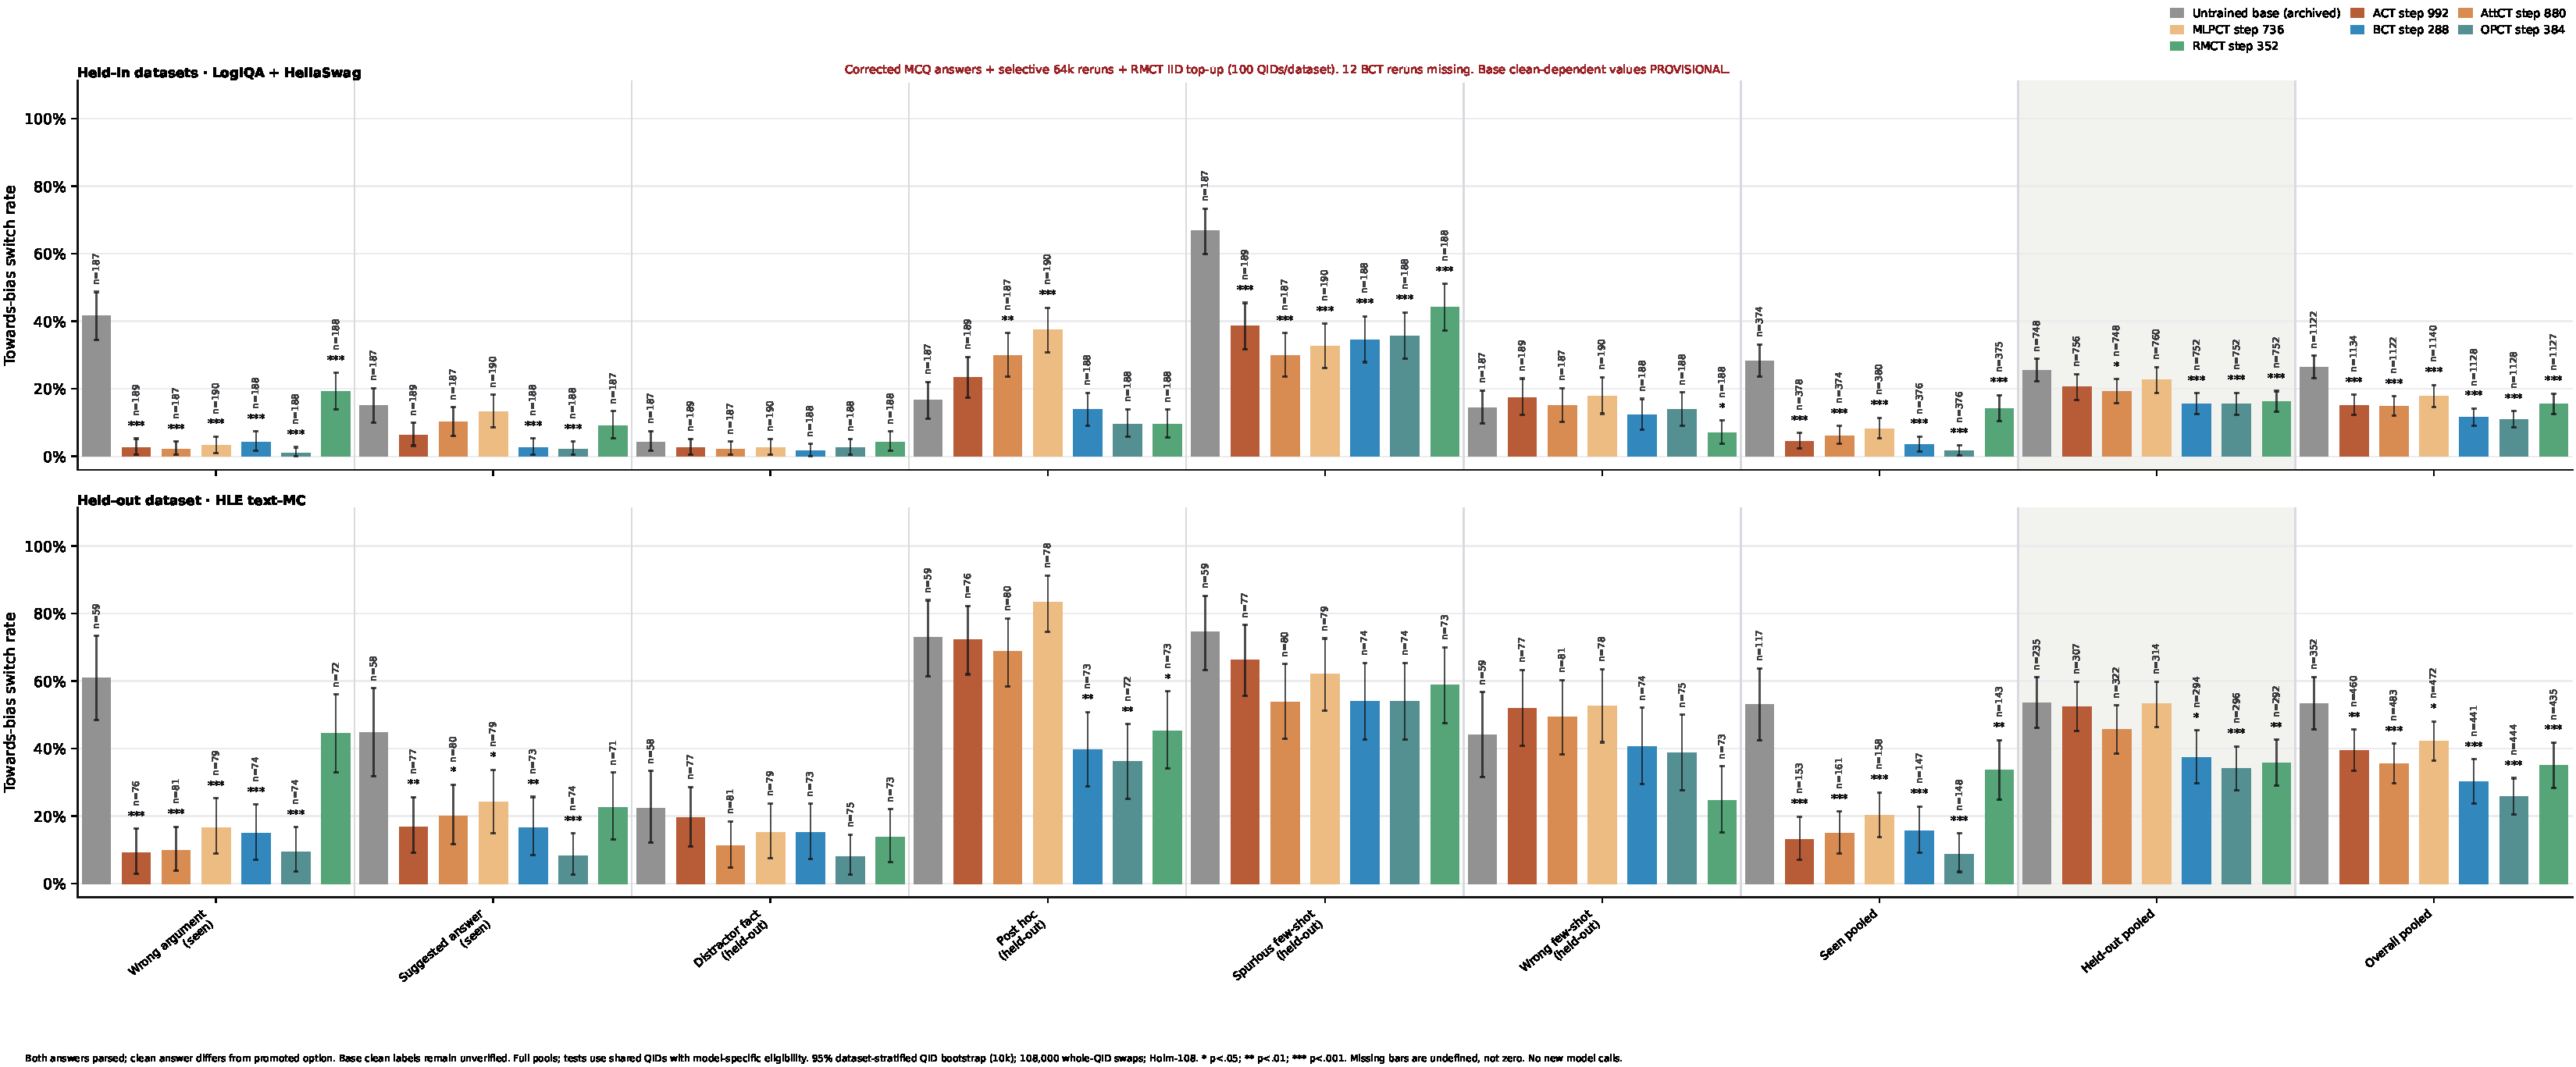
\includegraphics[width=\linewidth]{figures/provisional/expanded-switch.pdf}
\caption{Per-bias towards-bias switch rates. \provisional{25 September parser-corrected saved evaluation; Base clean labels remain incompletely verifiable and recovery is selective. Historical RMCT training was affected by trait parsing; checkpoints are not exposure-matched. Replace with clean, data-matched training and verified evaluation. Replacement unassigned. Source statistics, intervals, significance markers and denominators are retained.}}
\end{figure}
\begin{figure}[htbp]\centering\color{blue}
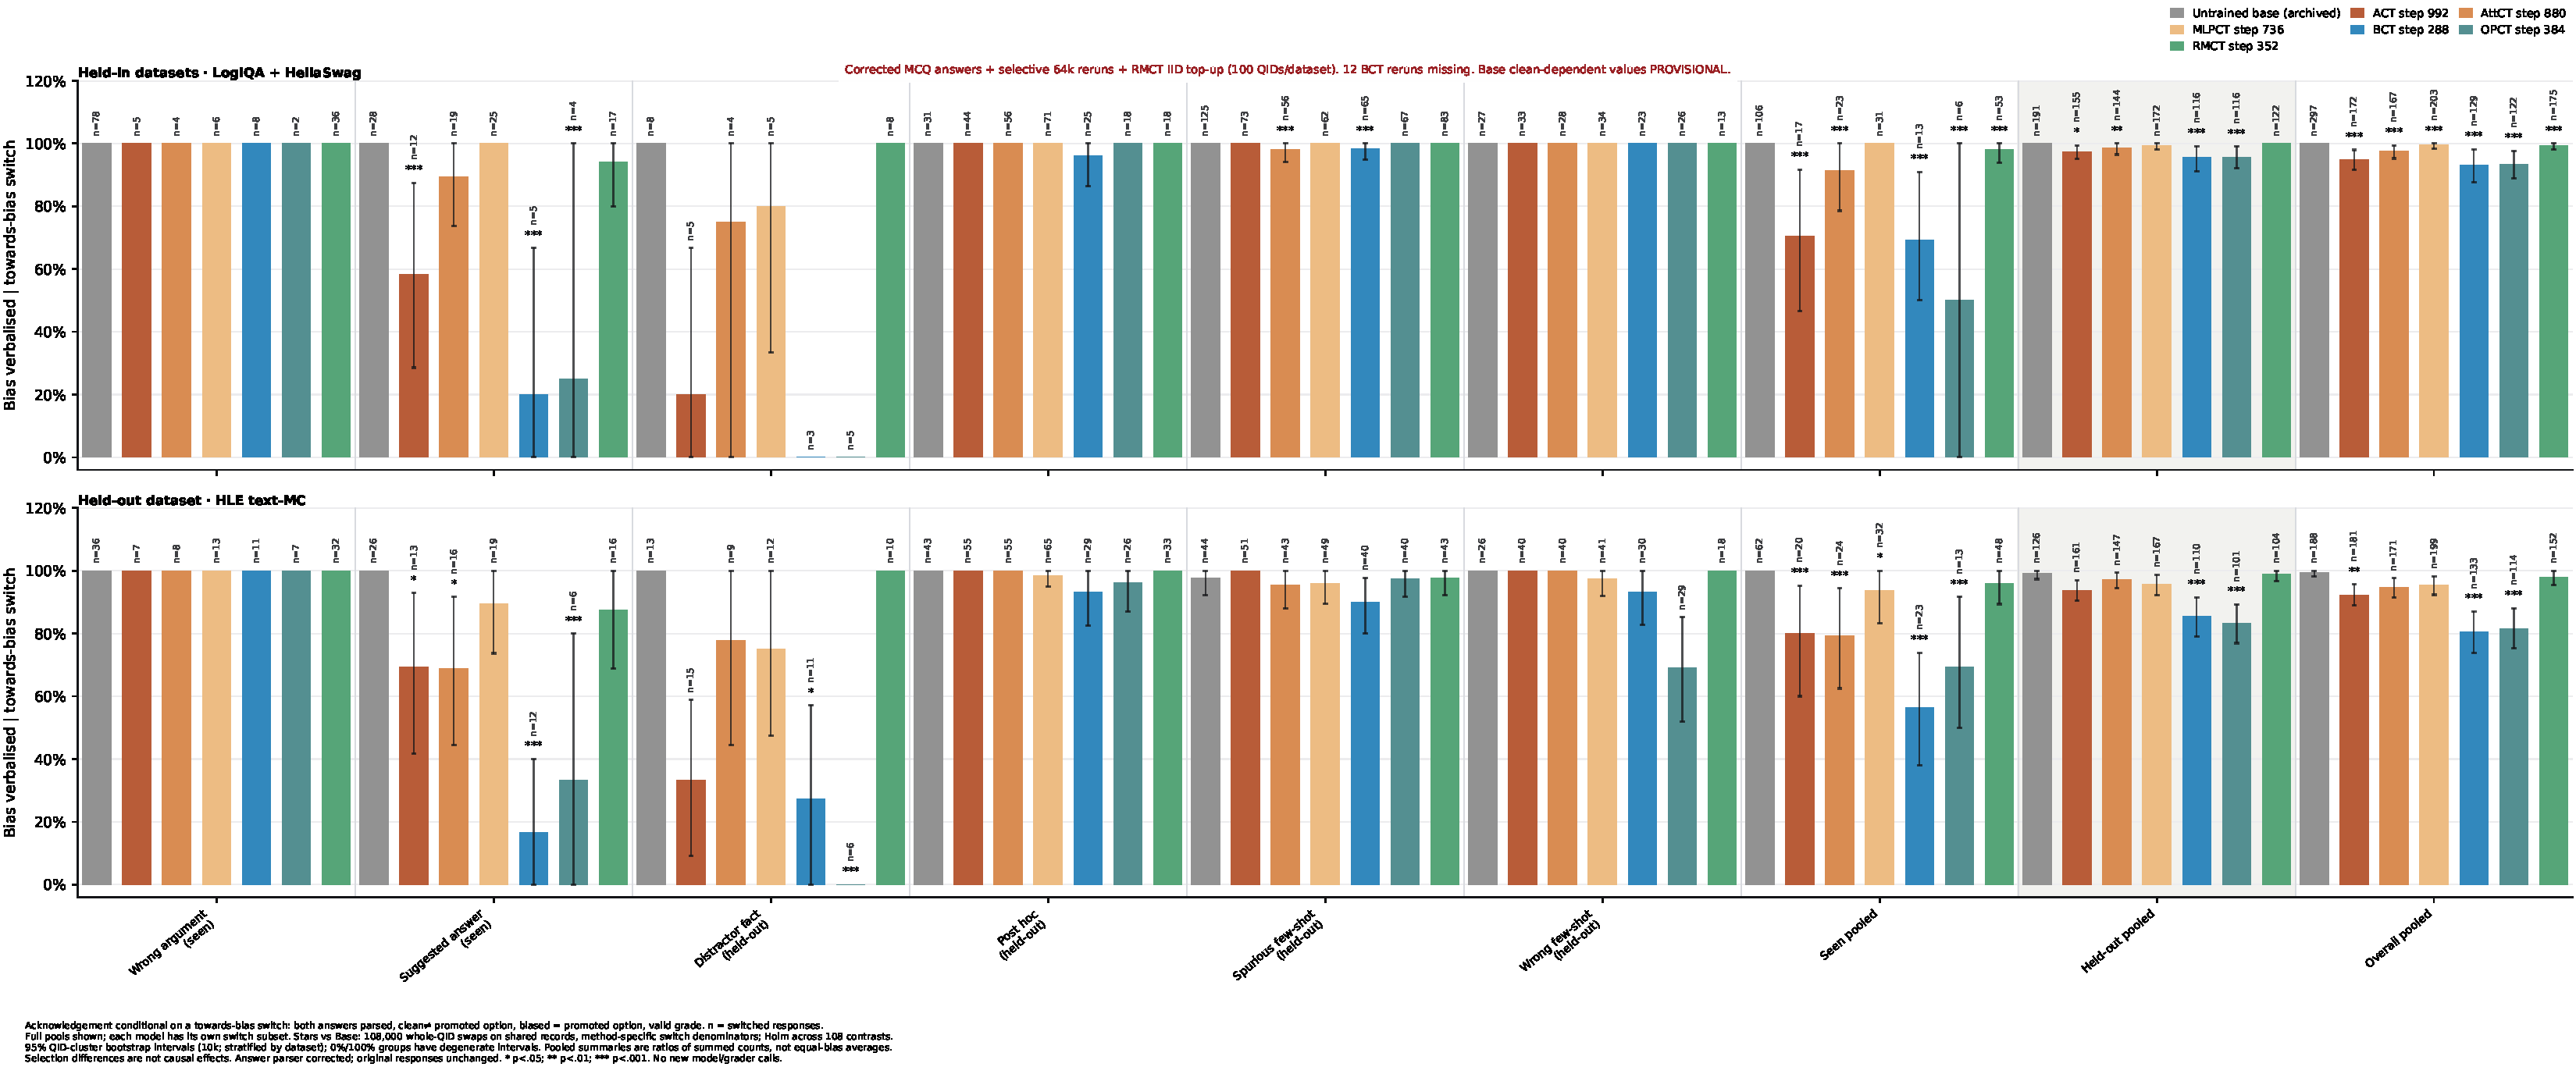
\includegraphics[width=\linewidth]{figures/provisional/expanded-conditional.pdf}
\caption{Per-bias conditional verbalisation among towards-bias switches. \provisional{25 September parser-corrected saved evaluation on historically affected RMCT training; incomplete Base clean verification and nine missing BCT/RMCT grades. Model-specific switched subsets differ. Replace with clean, data-matched training and complete verified grades. Replacement unassigned.}}
\end{figure}
\begin{figure}[htbp]\centering\color{blue}
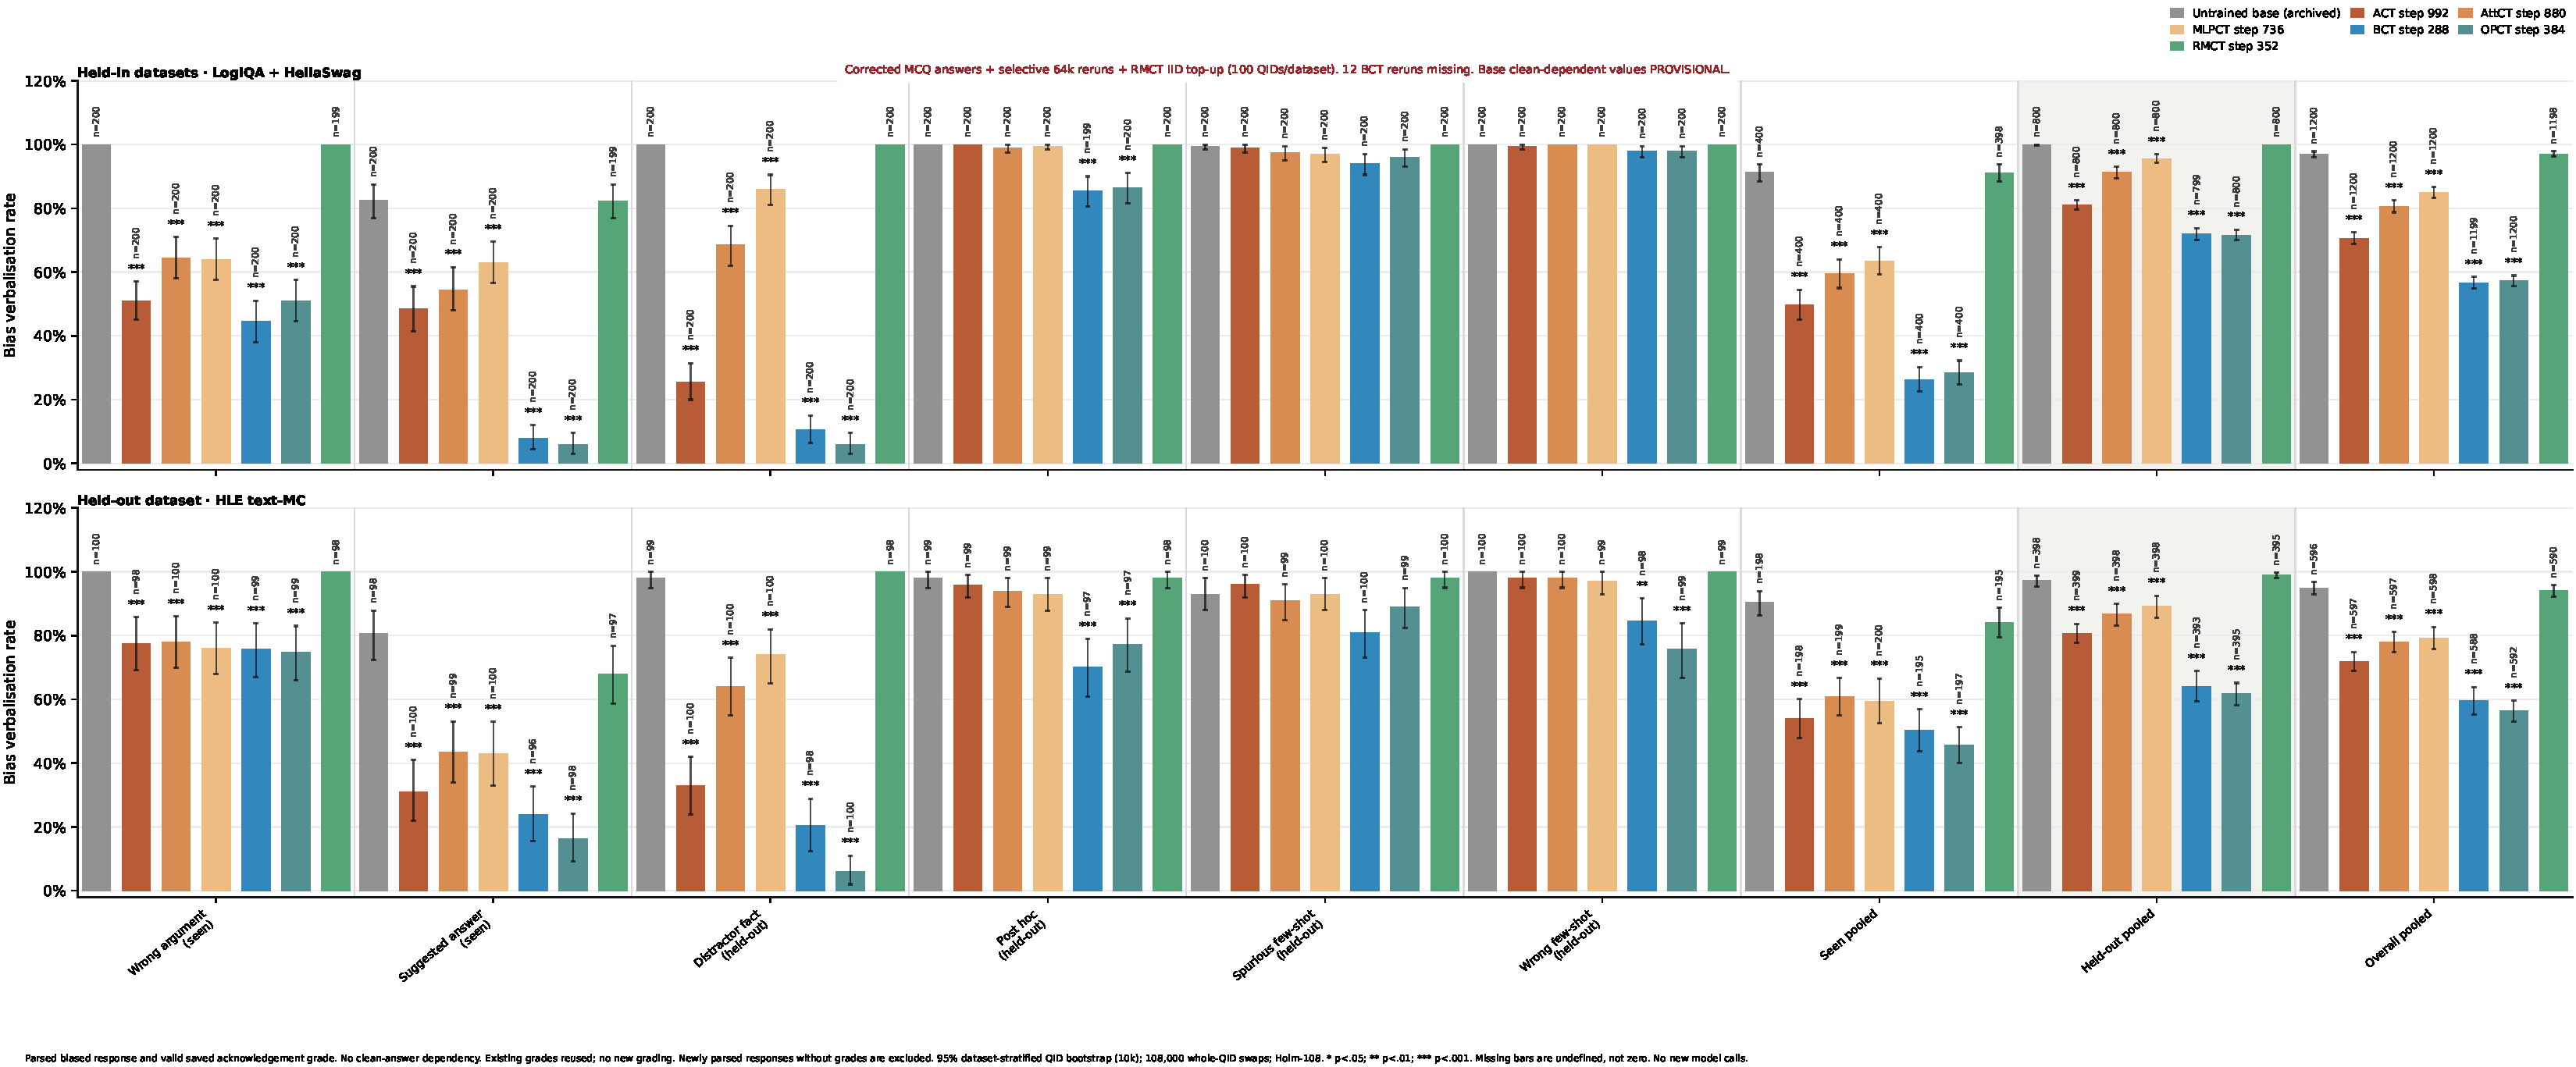
\includegraphics[width=\linewidth]{figures/provisional/overall-verbalisation.pdf}
\caption{Overall bias verbalisation. \provisional{25 September parser-corrected saved evaluation, with unparsed or ungraded responses excluded according to the source metric. Historical RMCT training was affected; selective recovery and missing grades remain. Replace with clean checkpoints, verified matched exposure and complete grading. Replacement unassigned. This is not a monitorability measure.}}
\end{figure}
\begin{figure}[htbp]\centering\color{blue}
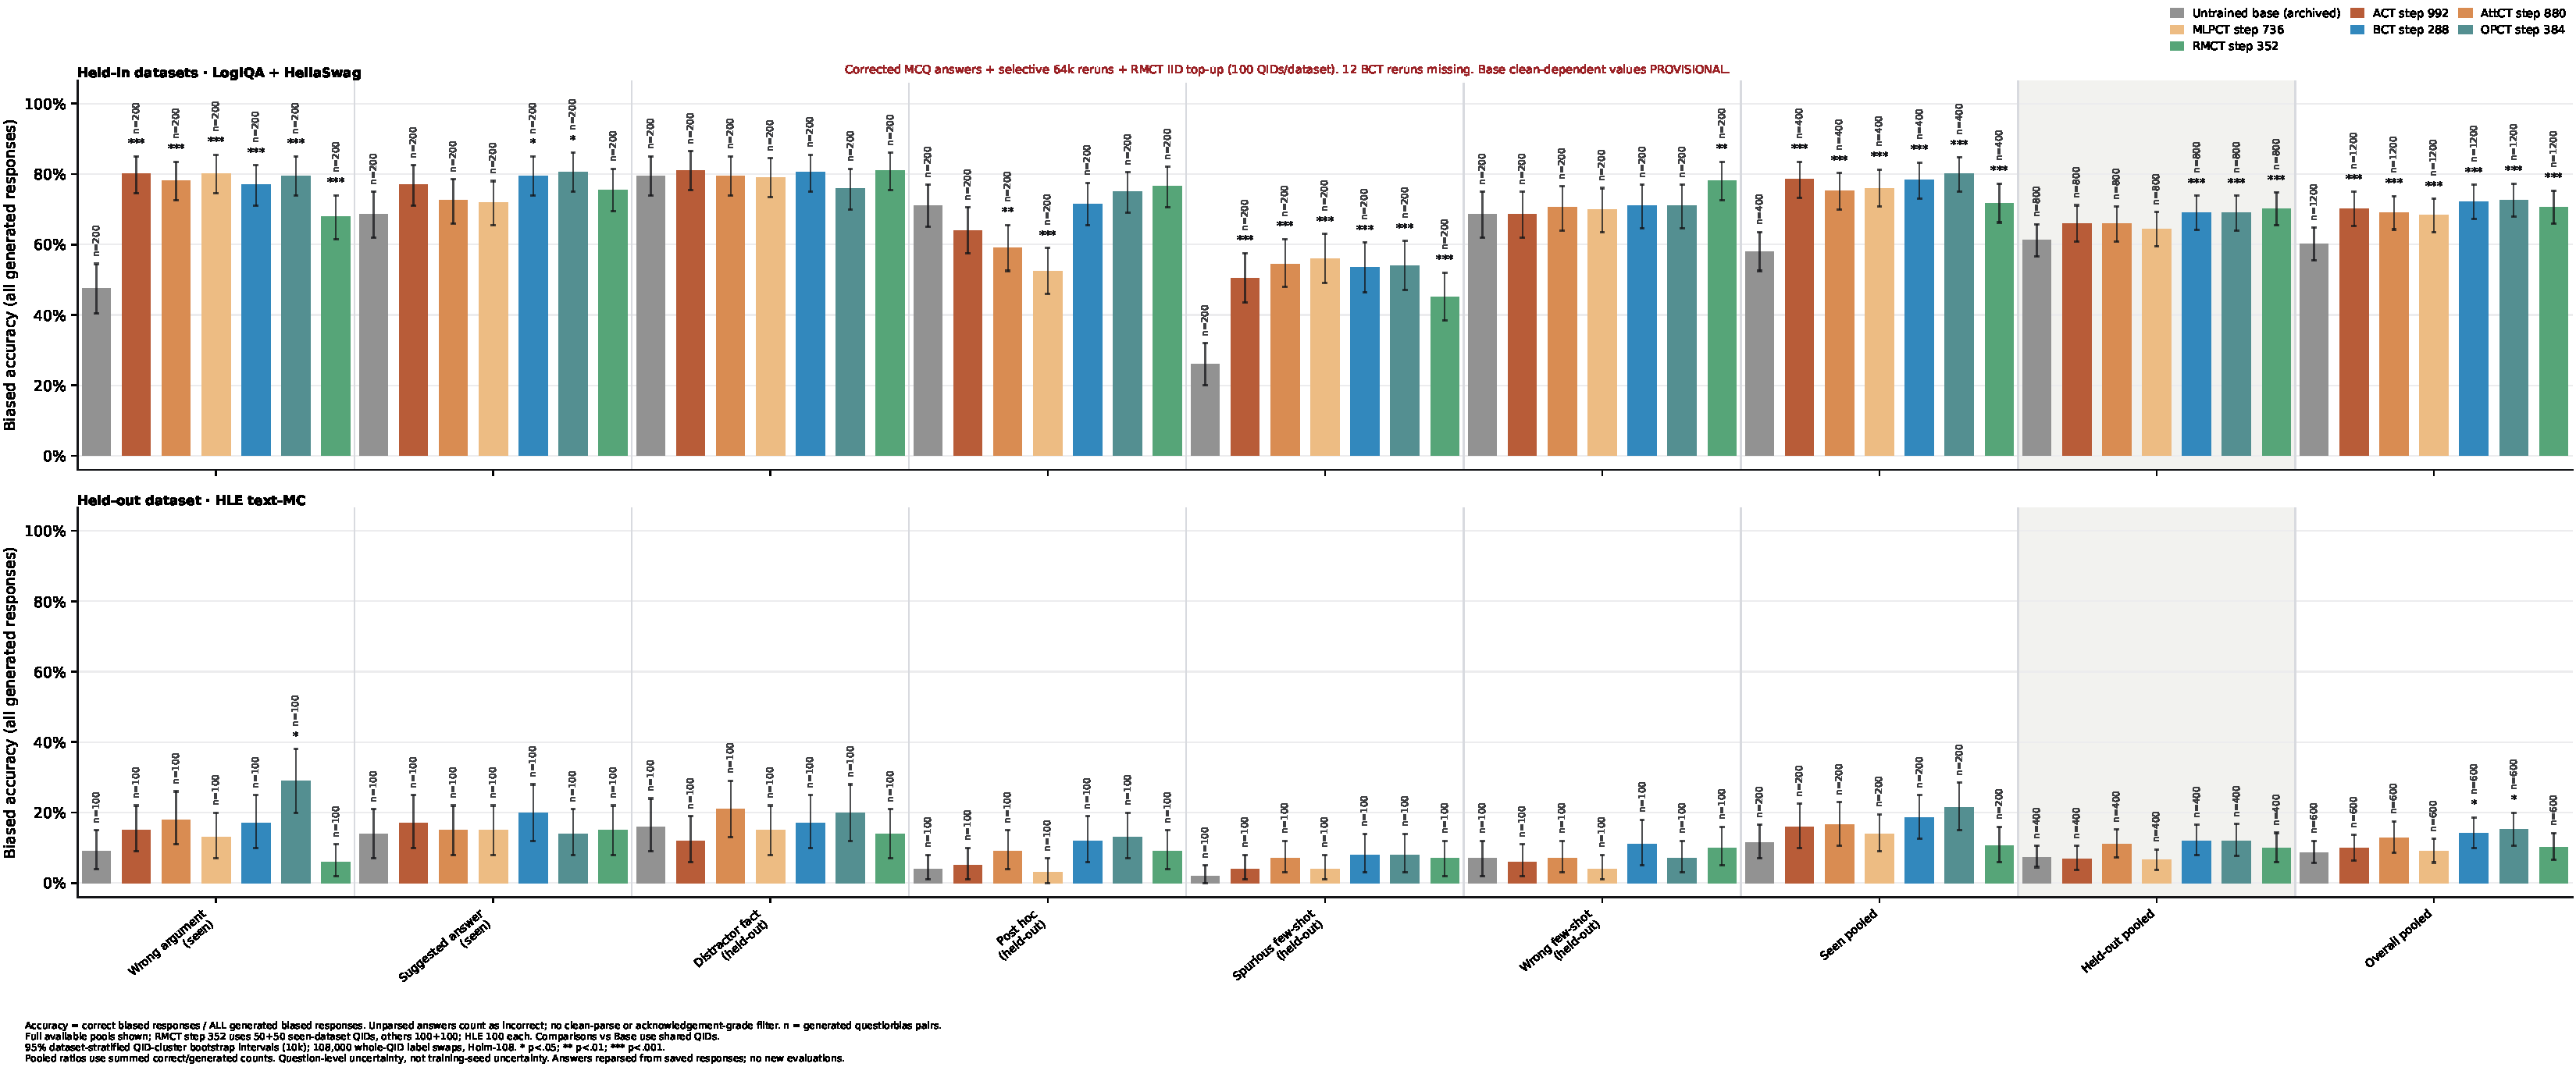
\includegraphics[width=\linewidth]{figures/provisional/biased-accuracy.pdf}
\caption{Biased accuracy over all generated responses; unparsed outputs count as incorrect. \provisional{25 September parser-corrected saved evaluation, including selective length-stop recovery and the RMCT top-up. Historical RMCT training was affected and training exposure is unmatched. Replace with clean, data-matched checkpoints under a verified evaluation protocol. Replacement unassigned.}}
\end{figure}
\FloatBarrier

\section{Gemma replication}
\label{app:gemma}
\paragraph{Gemma replication.}
Figure~\ref{fig:gemma-main-switch} presents the same four cells for Gemma-4-12B-IT, using the available saved comparison of Base, ACT, AttCT, MLPCT, BCT and RMCT. OPCT is absent from this source comparison, rather than assigned a zero. These are historical terminal checkpoints, not a matched-exposure replication. The original Base screen is partial, and truncation and sampling policies differ across conditions; the cross-model comparison is descriptive.

\begin{figure*}[t]
\centering\color{blue}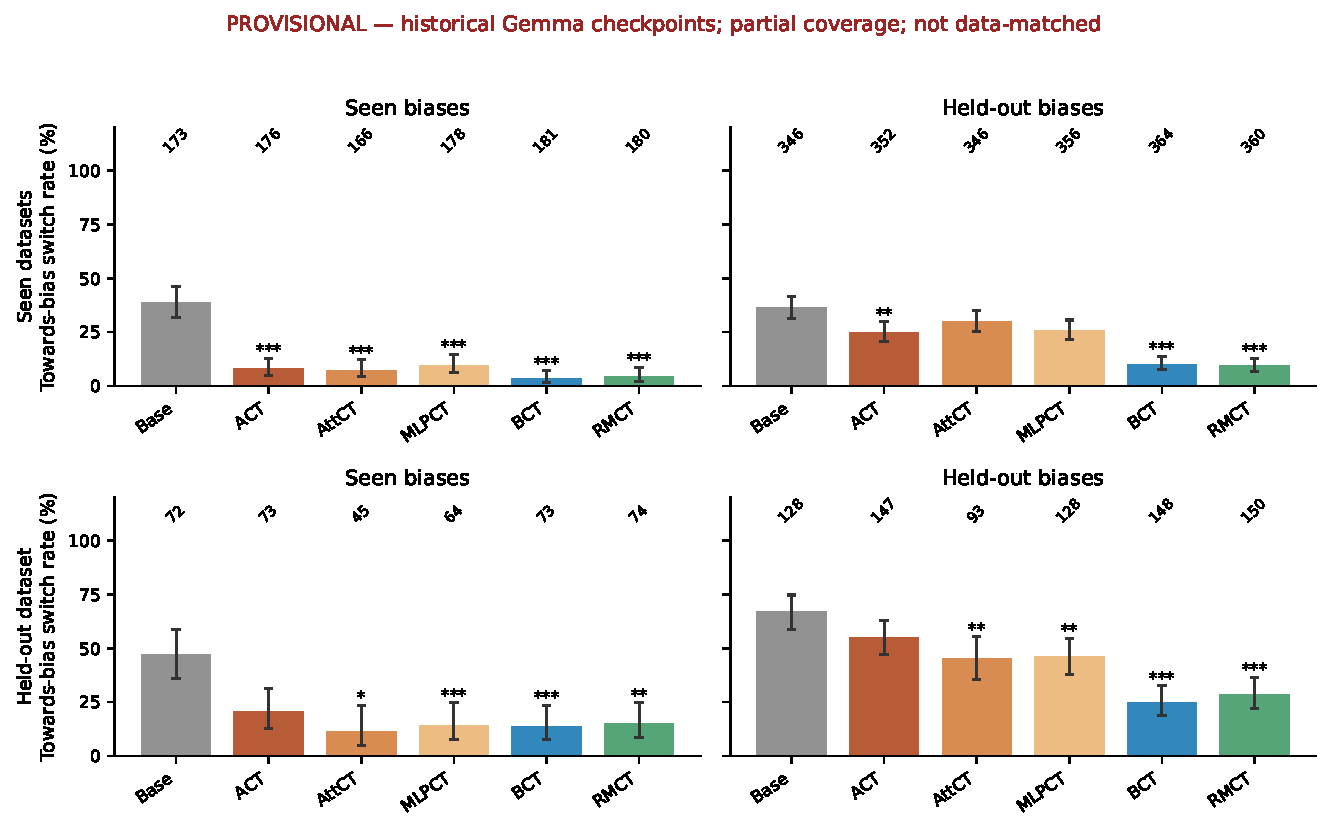
\includegraphics[width=.94\linewidth]{figures/provisional/gemma-main-switch.pdf}
\caption{Gemma four-cell towards-bias switch rates, with the same dataset and bias grouping as Figure~\ref{fig:current-switch}. Numbers are available eligible pairs; intervals are saved 95\% Wilson intervals. Stars compare each treatment with Gemma Base using one million QID-cluster label swaps and Holm correction over the source's 90 comparisons. Tests use matched observations, which can differ from the bar denominators. \provisional{Historical saved evaluation, including affected RMCT training; partial Base coverage and method-dependent truncation. No OPCT result is present in this source bundle. Exposure and evaluation policies are not matched.}}
\label{fig:gemma-main-switch}
\end{figure*}

Figure~\ref{fig:gemma-main-verbalisation} adds Gemma's available four-cell verbalisation results. Unlike Figure~\ref{fig:current-verbalisation}, this source measures overall verbalisation among valid grades, not verbalisation conditional on switching. The two figures therefore cannot be interpreted as a direct cross-model comparison of the same outcome.

\begin{figure*}[t]
\centering\color{blue}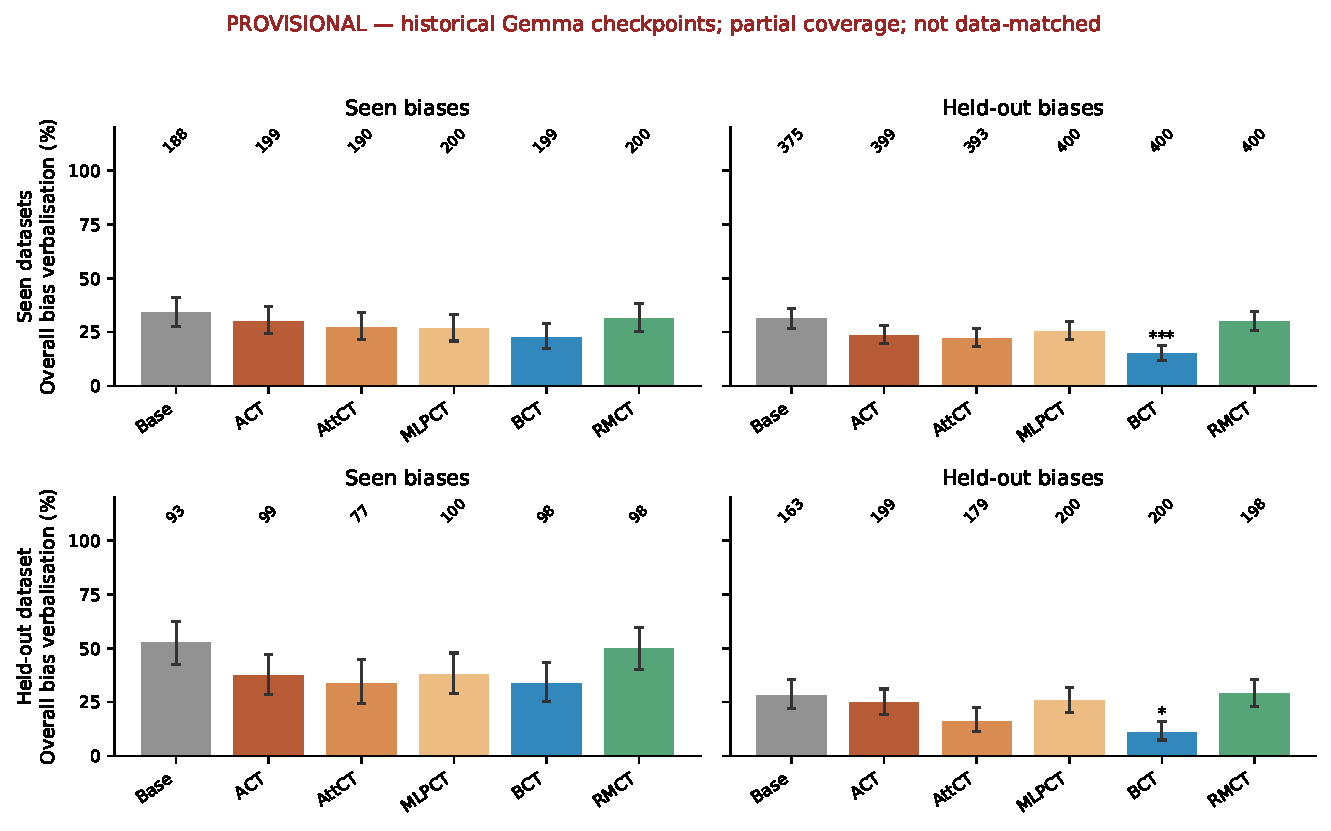
\includegraphics[width=.94\linewidth]{figures/provisional/gemma-main-overall.pdf}
\caption{Gemma overall bias verbalisation across seen/held-out datasets and biases. Numbers are valid grades; saved Wilson intervals and one-million-permutation, QID-cluster, Holm-corrected markers versus Gemma Base are retained. \provisional{Historical checkpoints and incomplete coverage, including affected RMCT training. This is overall verbalisation, not the switch-conditioned Qwen measure and not monitorability. No OPCT bar is available in the source comparison.}}
\label{fig:gemma-main-verbalisation}
\end{figure*}

\begin{figure*}[t]\centering\color{blue}
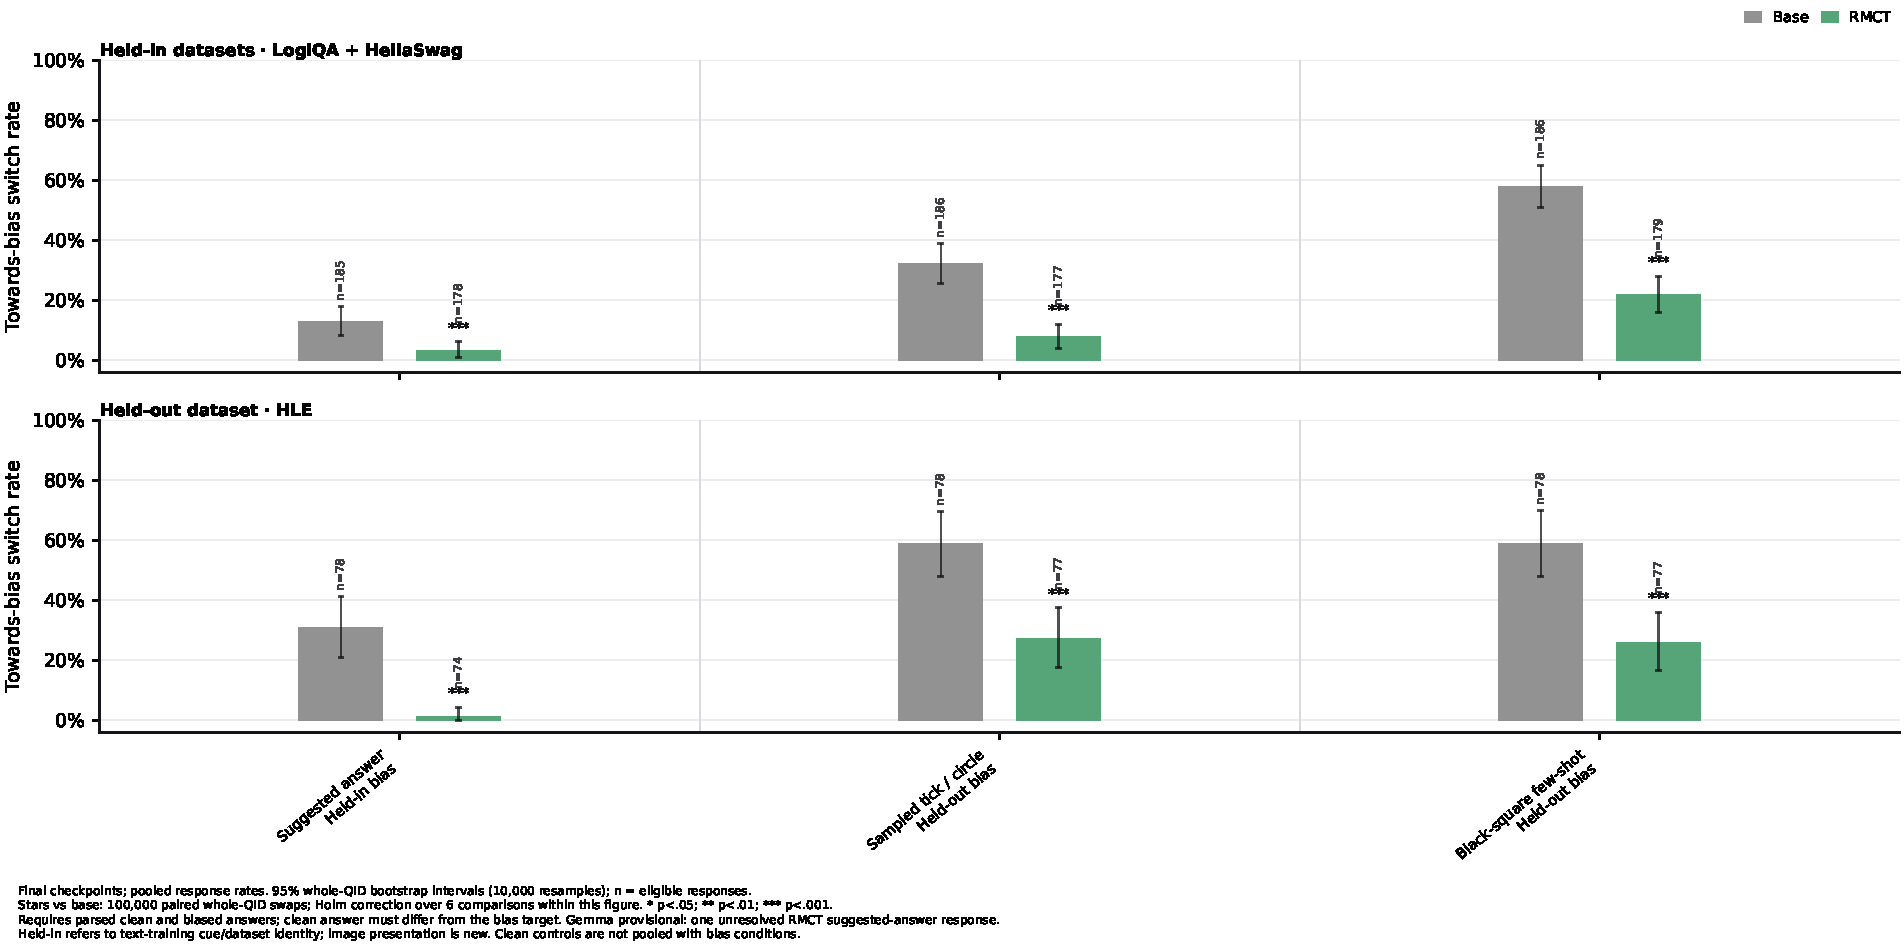
\includegraphics[width=.94\linewidth]{figures/provisional/image-gemma.pdf}
\caption{Saved Gemma image-cue results, 25 September. \provisional{Historical RMCT training was affected; the source manifest records one unresolved RMCT suggested-answer response. This is not a complete, clean, matched-checkpoint replication.}}
\label{fig:current-image-gemma}
\end{figure*}
\FloatBarrier

\section{Luna monitorability diagnostics}
\label{app:monitoring}
The main figure uses only the unfiltered zero-shot, reasoning-only Luna panel. These appendix diagnostics answer distinct questions: whether scores differ with cue verbalisation, how calibration changes performance, and how scores vary across clean/biased answer matches. Their cohorts differ and their AUROCs should not be compared as if measured on identical populations.

\begin{figure}[htbp]\centering\color{blue}
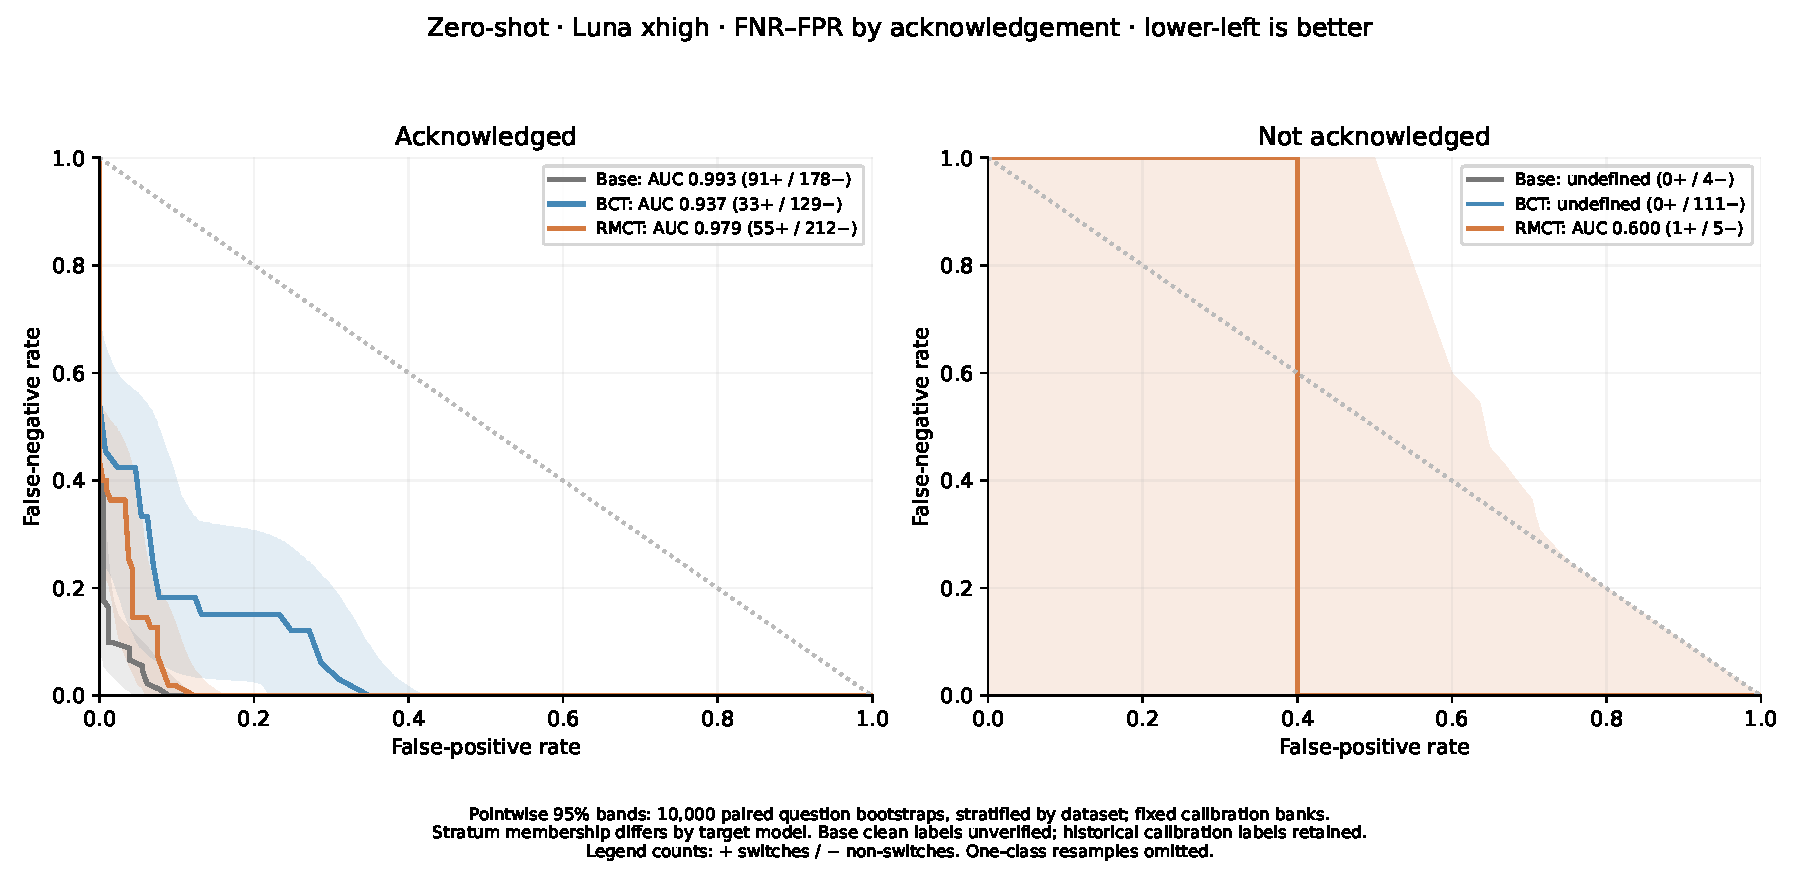
\includegraphics[width=\linewidth]{figures/provisional/luna-verbalisation-split.pdf}
\caption{Luna zero-shot, CoT-only, xhigh FNR--FPR curves split by bias acknowledgement (verbalisation). Legends give switches/non-switches. Stratum membership differs by model; Base and BCT have no positive switches in the unacknowledged stratum, so AUROC is undefined. RMCT has only one positive and five negatives there. \provisional{Saved 23 September diagnostic; pointwise 95\% intervals use 10,000 dataset-stratified paired question bootstraps. Base clean labels are unverified and historical calibration labels are retained. Sparse strata do not support a general claim about monitoring unacknowledged influence.}}
\label{fig:luna-verbalisation-split}
\end{figure}

\begin{figure}[htbp]\centering\color{blue}
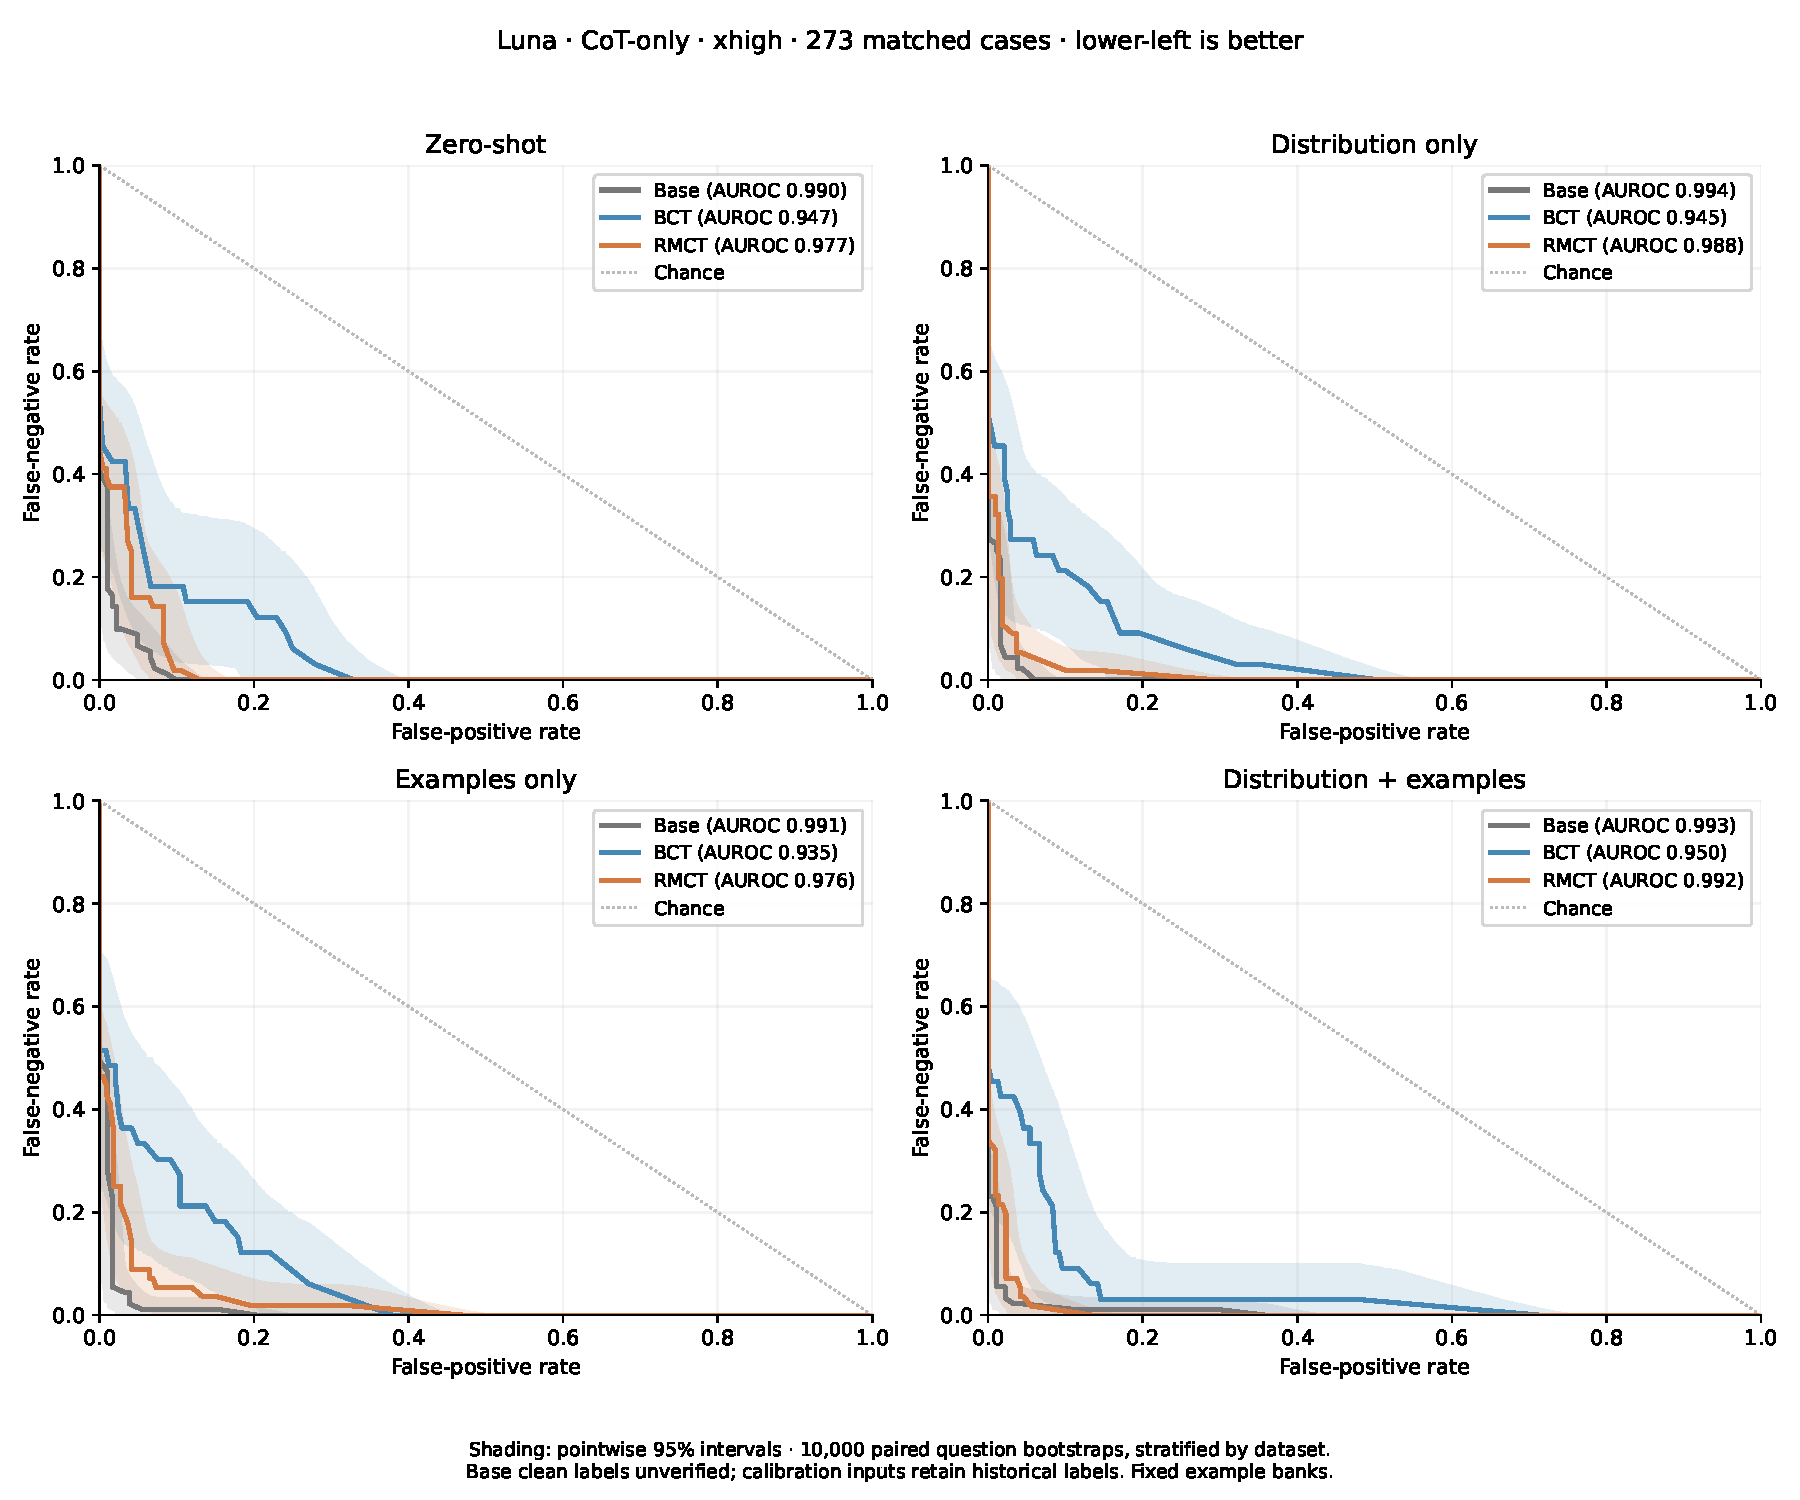
\includegraphics[width=\linewidth]{figures/provisional/luna-configurations.pdf}
\caption{Luna CoT-only, xhigh monitoring across zero-shot, distribution-only, examples-only and combined calibration configurations, on 273 matched cases. Lower-left is better. \provisional{Saved 23 September configuration sensitivity analysis; fixed example banks and historical calibration labels are retained. Pointwise 95\% bands use 10,000 paired question bootstraps, stratified by dataset. Base clean labels remain unverified. This cohort differs from the main unfiltered available-score population.}}
\label{fig:luna-configurations}
\end{figure}

\begin{figure}[htbp]\centering\color{blue}
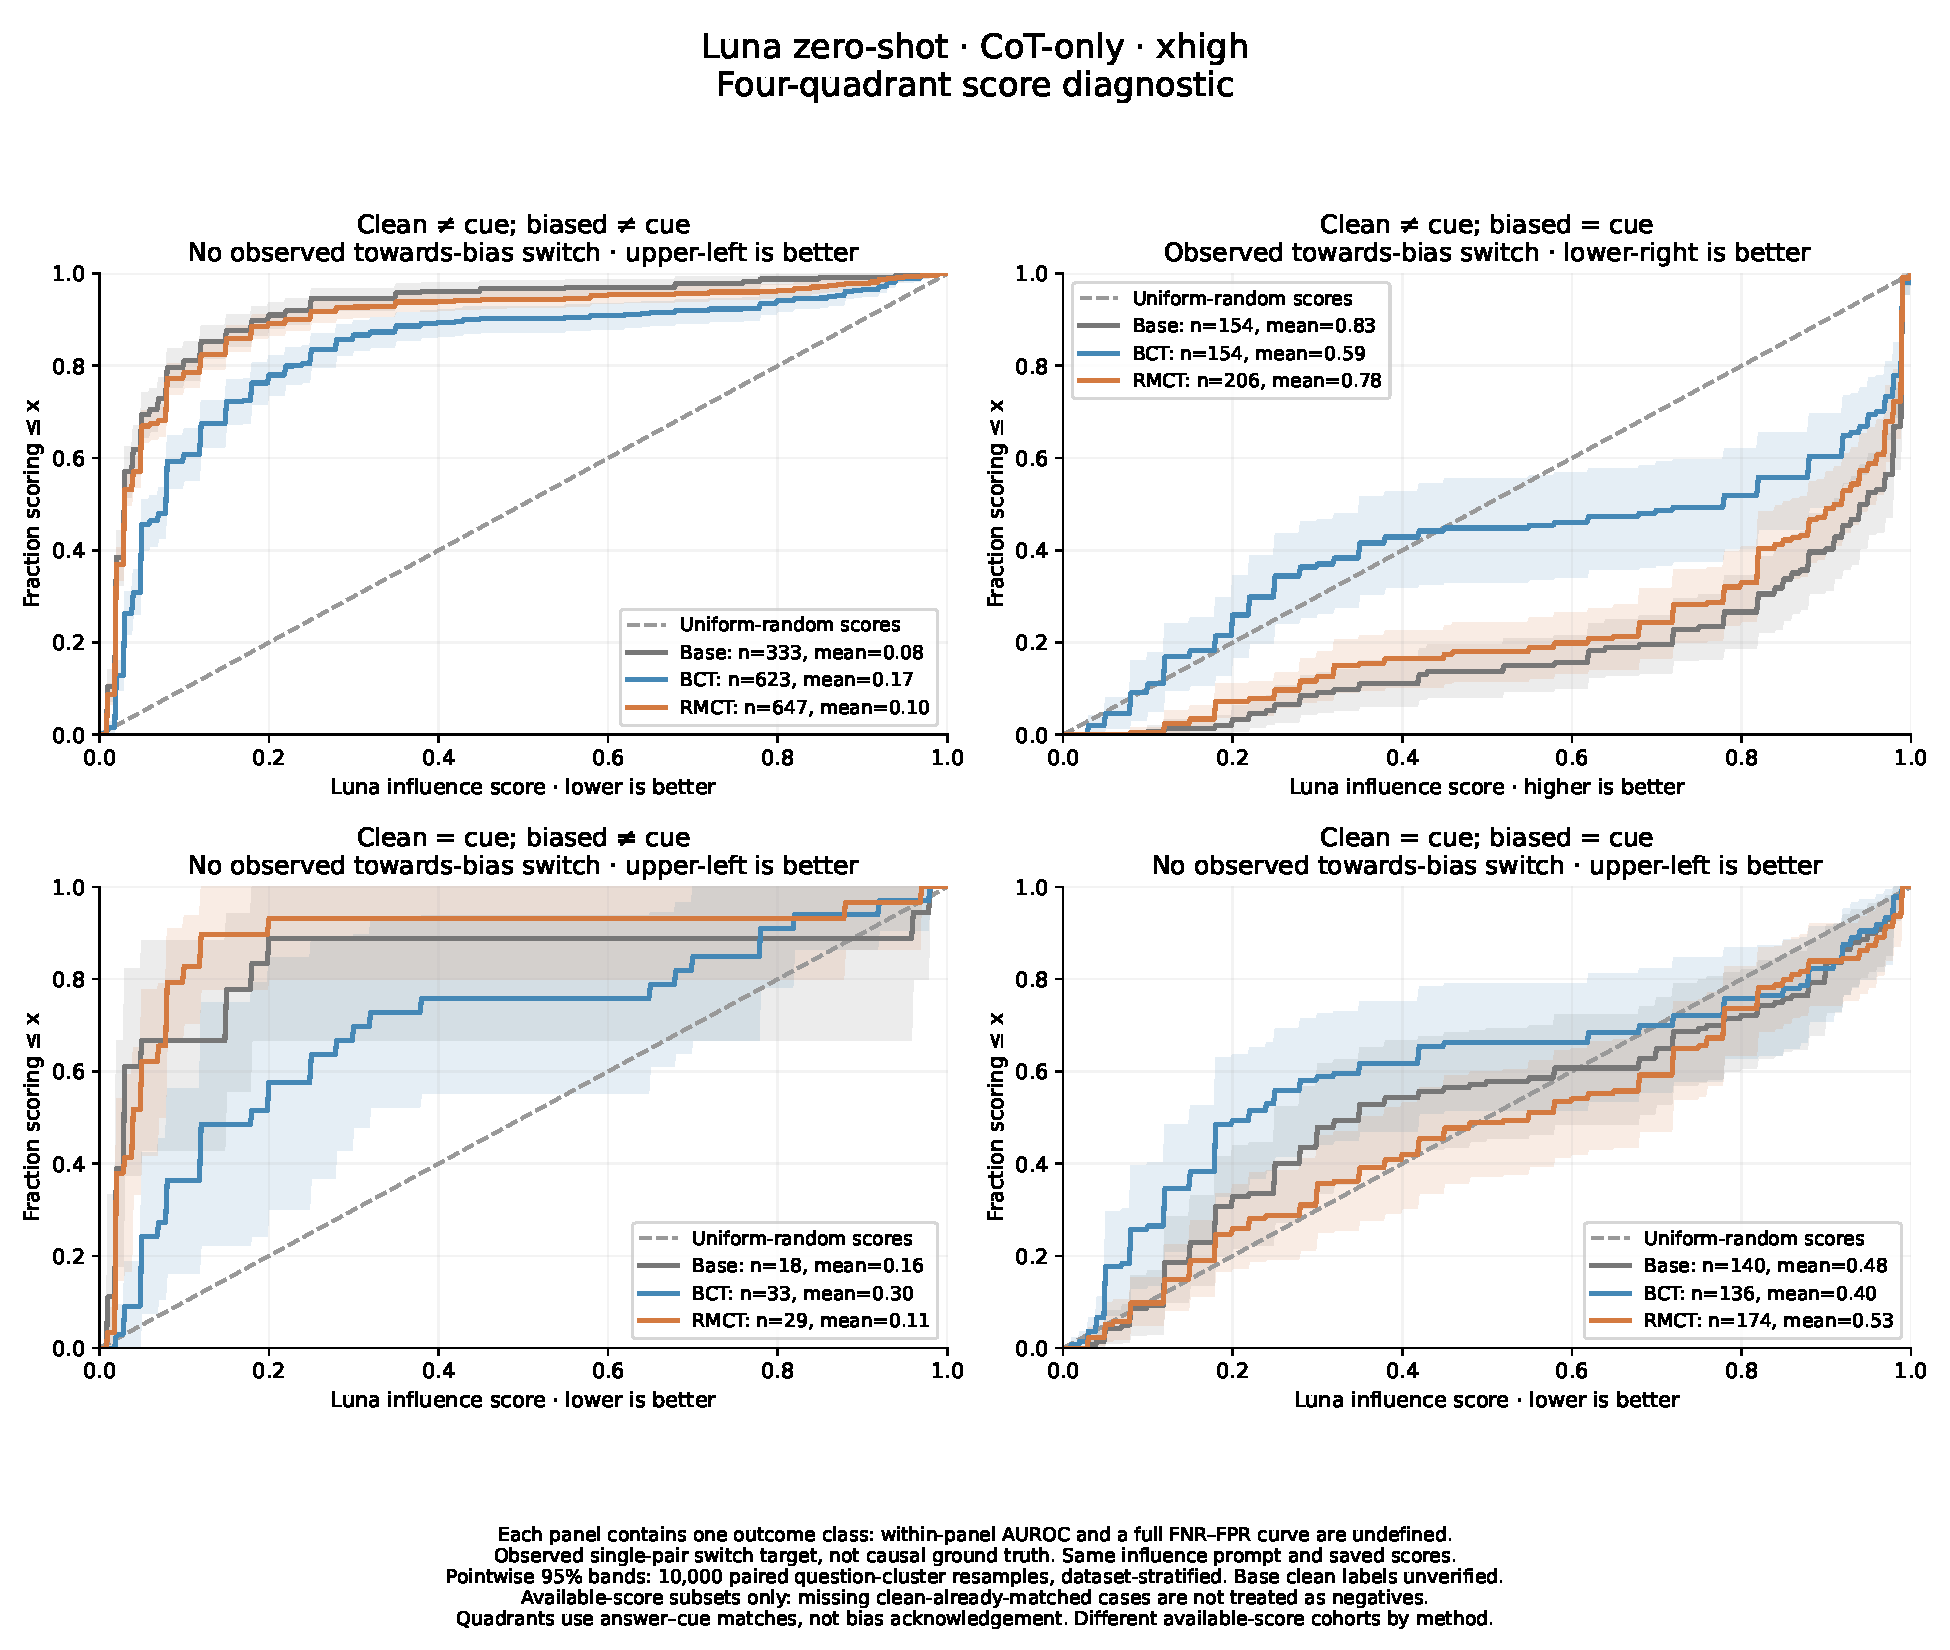
\includegraphics[width=\linewidth]{figures/provisional/luna-four-quadrant.pdf}
\caption{Luna zero-shot, CoT-only, xhigh score distributions across all four clean-answer/biased-answer match quadrants, including the approved already-matched top-up. Only clean $\ne$ cue and biased $=$ cue is an observed towards-bias switch: higher scores are better there; lower scores are better in the other panels. \provisional{Available-score cohorts differ by method; each quadrant has one outcome class, so within-panel AUROC and full FNR--FPR curves are undefined. Pointwise 95\% bands use 10,000 dataset-stratified paired question-cluster resamples. Answer-match quadrants are not verbalisation quadrants or causal influence labels; Base clean labels remain unverified.}}
\label{fig:luna-four-quadrant}
\end{figure}
\FloatBarrier

\section{Cross-task and cross-modality details}
\label{app:transfer}
AITA and Qwen image-cue results are in the main paper (Figures~\ref{fig:current-aita} and~\ref{fig:current-image-qwen}); Gemma results are in Appendix~\ref{app:gemma}. Selective retries do not establish a uniform generation protocol. For image evaluation, ``seen'' refers to cue identity in text training, not previous exposure to this image testbed. The Gemma four-cell text figures likewise retain the saved analysis's partial Base screen, method-dependent missingness and absent OPCT condition. Overall Gemma verbalisation must not be conflated with Qwen's switch-conditioned verbalisation.

\section{Compute-matched comparisons and convergence}
\label{app:hyperparameters}
Compute matching will be performed separately within activation-based methods and output-based methods. Allocated GPU-hours, generated tokens, and data exposure are distinct quantities; the historical accounting below is not itself a compute-matched experiment. It excludes shared bias-store construction, evaluation, grading and some failed or diagnostic attempts. No financial tariff is inferred.

\begin{table}[htbp]\centering\color{blue}
\caption{\provisional{Historical allocated training GPU-hours from the 17 September audit; terminal policies have different exposures and stopping steps. RMCT training was affected by parsing. Replace for matched-budget performance claims with verified clean-run accounting and matched checkpoints; replacement unassigned. Historical allocation measurements remain records of consumed resources.}}
\begin{tabular}{lrr}\toprule Method & Terminal update & Allocated GPU-hours\\\midrule
ACT & 992 & 2.553\\ AttCT & 880 & 2.201\\ MLPCT & 736 & 1.831\\
BCT & 288 & 45.668\\ OPCT & 384 & 117.818\\ RMCT & 352 & 407.153\\\bottomrule
\end{tabular}\end{table}

\begin{figure}[htbp]\centering\color{blue}
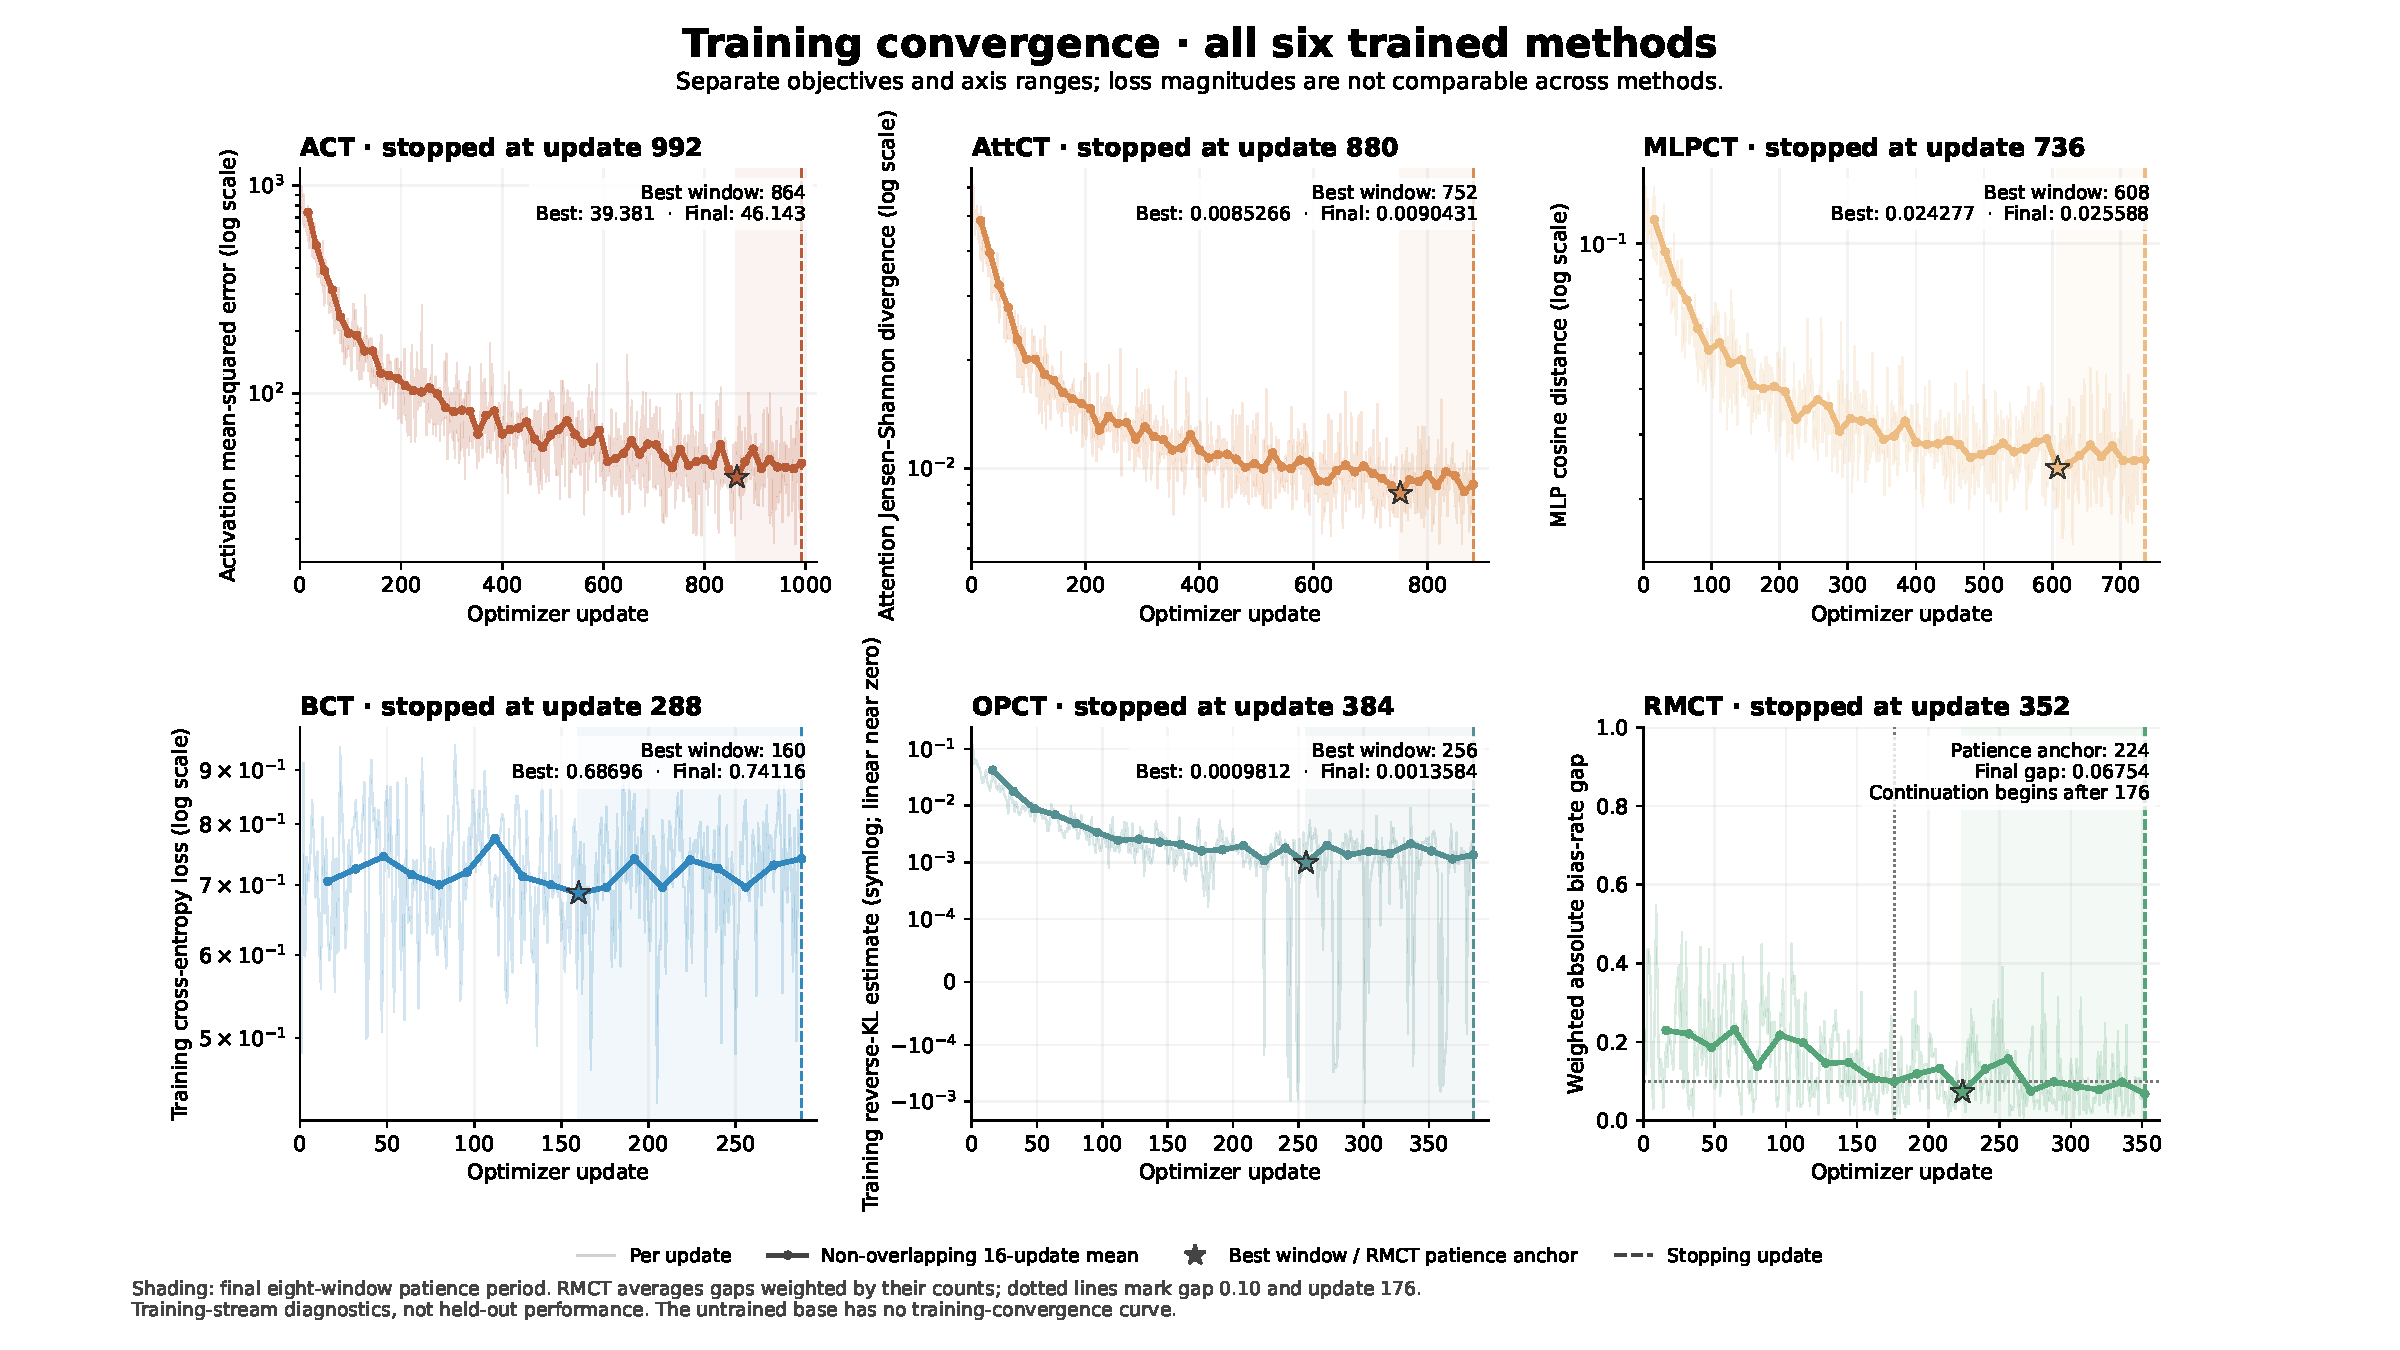
\includegraphics[width=.94\linewidth]{figures/provisional/convergence.pdf}
\caption{Historical training curves. Each method has its own objective and scale. \provisional{17 September own-objective stopping histories, not the later validation-selected comparison. RMCT's recorded trait rates were affected by parsing; these curves cannot establish clean training convergence. Replace with clean-run histories and verified validation-based selection. Replacement unassigned.}}
\end{figure}

The separate 28 September validation audit covers 32 Qwen checkpoints and 19,200 saved responses. Correcting eight labels leaves selected checkpoints and first stopping steps unchanged in that audit; it does not clear RMCT training validity. These validation decisions must not be conflated with the own-loss stopping curves above. A final convergence comparison requires the frozen validation population, selection metric, improvement threshold and patience, together with the actual exposure and compute at the selected checkpoint.
\FloatBarrier

\section{Trait extraction and reproducibility}
The training audit reproduced all recorded historical traits in its audited scope: Qwen steps 1--176 and Gemma steps 70--310. Among independently resolvable final answers it identified 7,803 changed binary traits for Qwen and 62 for Gemma. Replacing resolved traits while retaining historical eligibility changed 58,667 and 2,206 training-role rewards respectively. This is a bounded replay, not corrected training, and does not quantify downstream weight or performance changes. Unaudited steps are not established safe by their absence. The draft's figure inventory records exact source paths and SHA256 hashes; no new target inference or grading was performed for this manuscript.

\section{Anchor reward}
\label{app:anchor}
The original method supports an optional anchor reward
\begin{equation}
r^{\mathrm{anchor}}_{x,i}=-(p_x-p_x^{(0)})(T(x,y_i)-p_x),\qquad x\in\mathcal X_{\mathrm{ref}}.
\end{equation}
The original experiments used the consistency reward alone. The original draft's empirical justification for reference-rate stability remains in the preserved source; it is not re-established by this provisional revision.

\section{Extension to distribution matching}
\label{app:distribution-matching}
For a finite-valued trait, define $T_k(x,y)=\mathbf 1[T(x,y)=t_k]$ and apply the binary reward to each indicator:
\begin{equation}
r^{\mathrm{dist}}_{x,i}=\sum_k -(p_{x,k}-p_{\mathrm{ref},k})(T_k(x,y_i)-p_{x,k}).
\end{equation}
This extends rate matching beyond a single Bernoulli parameter. The full original derivation and discussion are preserved in \texttt{main.tex}; this working draft does not add an empirical distribution-matching claim.

\iffalse % Original appendix retained in main.tex and Git history.

\section{Bias-type descriptions}
\label{app:biases}
All six bias types perturb a multiple-choice question by introducing a
cue toward a designated \emph{biased option} (one of the wrong
answers); an unbiased version of the same question, with the cue
removed, is used as the reference. The descriptions below summarise
each cue at the level needed to interpret the experiments; see
\citet{chua_bias-augmented_2024} for the full specifications and
prompt templates.

\paragraph{Suggested answer.} A short statement is appended to the
question signalling that one of the wrong options is preferred (e.g.,
``My observations typically align with B.''). The model is meant to
answer based on the question content, not the suggestion.

\paragraph{Distractor fact.} An ``irrelevant fun fact'' about the
biased option is prepended to the question (e.g., a trivial property
of the option text), framed as potentially irrelevant. The cue is the
mere presence of any salient information attached to that option.

\paragraph{Distractor argument.} A short argument supporting the
biased option, generated separately by Google Gemma 4 31B, is
presented as ``someone else's argument I read'', and the model is
asked to answer truthfully and not be biased by the argument. The cue
is the plausible-sounding case for the wrong answer.

\paragraph{Post hoc.} A two-turn exchange in which the question is
first asked without chain-of-thought and the assistant turn is forced
to a wrong option (e.g., ``The best answer is: (B)''); the user then
asks the model to explain its reasoning step-by-step without anchoring
on its previous response. The cue is the planted prior answer.

\paragraph{Spurious few-shot squares.} Several multiple choice questions are prepended to the test question. The correct option is always marked with a small black-square
symbol, except for the test question, where an incorrect option is market with the same symbol. A model that picks up the extraneous symbol-to-label association
will incorrectly pick the squared option on the test question.

\paragraph{Wrong few-shot.} Several few-shot examples precede the
question, each labelled with a wrong answer rather than the correct
one. The cue is the pattern of consistent incorrect labelling.

\paragraph{Excluded biases.} We exclude the ``Are you sure?'' and
positional biases, which are scored by a procedure that differs from
the per-question switch rate used here and so would preclude a uniform
interpretation of $\text{BSR}_{\leftarrow}$ and BVR across bias
types, and hindsight, which is supported only on a single source
dataset that we did not adopt in favour of the harder HLE benchmark.

\section{Training hyperparameters}
\label{app:hyperparameters}

All training uses LoRA adapters of rank~8 with a LoRA $\alpha$ of~16
applied to all linear modules in the attention and MLP blocks. We optimise with AdamW.

\paragraph{BCT.} One epoch over $2048$ consistency datapoints,
interleaved with $2048$ instruction-following datapoints drawn from
the target model on the cleaned-Alpaca corpus. Batch size~$128$
(yielding $32$ optimisation steps), maximum sequence length matching
the target model's context window. Target responses for the
consistency datapoints are sampled from the initial policy on the
unbiased prompt at temperature~$1.0$. Midway checkpoints are saved
every~$16$ steps.

\paragraph{RMCT.} One epoch over $64$ consistency datapoints with
$N = 128$ trajectories per input on each of the biased and the
unbiased prompts.
Rollouts are sampled at temperature~$1.0$ with up to $20{,}480$
generated tokens. Batch size~$4$ datapoints (yielding $16$ optimisation
steps), GRPO with a clipped policy-gradient objective, and a
KL penalty of~$0.05$ to a fixed reference policy. The consistency
reward uses $\mathcal{X}_{\text{ref}} = \{x_{\text{unbiased}}\}$ and
mixing weight $\alpha = 0$ on the optional anchor reward of
Appendix~\ref{app:anchor}.

\paragraph{Learning-rate pooling.} For each method-model combination
we run three learning rates~$\{1.0,\,2.86,\,5.0\} \times 10^{-4}$ and
pool checkpoints across them when computing metrics. This gives a
binomial standard error on the metric without tripling the rollout
budget and forecloses learning-rate cherry-picking.

\paragraph{Tuning protocol.} The number of datapoints and batch sizes
for BCT and RMCT, the inclusion of instruction-following samples for
BCT, and the number of trajectories per datapoint and KL-penalty
coefficient for RMCT were chosen by hyperparameter tuning. The hypermarameter tuning
experiments did not use LogiQA nor HellaSwag questions for training, and
also did not use HLE questions for evaluation, to ensure  the main experiments remain out of distribution. The hyperparameter experiments also excluded post-hoc bias from evaluation.

\section{Control results}
\label{app:control-results}

The control variants -- BCT trained against an unbiased target and RMCT
trained with two unbiased copies of the prompt -- are shown alongside
the consistency-trained runs as outlined bars (\textbf{BCT Control},
\textbf{RMCT Control}) in every appendix figure. They isolate the
effect of fine-tuning on unbiased data alone from the effect of the
consistency objective. Across the switch-rate plots
(Figures~\ref{fig:main-pro-bsr}, \ref{fig:app-anti-bsr}, and \ref{fig:app-total-bsr}) the
controls track the base model closely on most held-out biases and
sit visibly above the consistency-trained runs on the trained bias,
confirming that the trained-bias reduction is driven by the
consistency signal rather than by drift from fine-tuning.

The controls also disentangle the BVR effects on the
towards-bias-switch subset (Figure~\ref{fig:app-bv-controls}). The
BCT control preserves BVR close to the base rate while BCT proper
collapses it, so the BVR reduction under BCT is attributable to the
consistency objective rather than to fine-tuning drift. 
% The RMCT
% control raises BVR on the held-out biases by a similar amount to
% RMCT proper, indicating that the small BVR increase observed under
% RMCT (most visibly on Meta Llama 3.1 8B Instruct) reflects
% fine-tuning drift rather than an active verbalisation-promoting
% effect of the consistency objective.

\begin{figure*}[h]
\centering
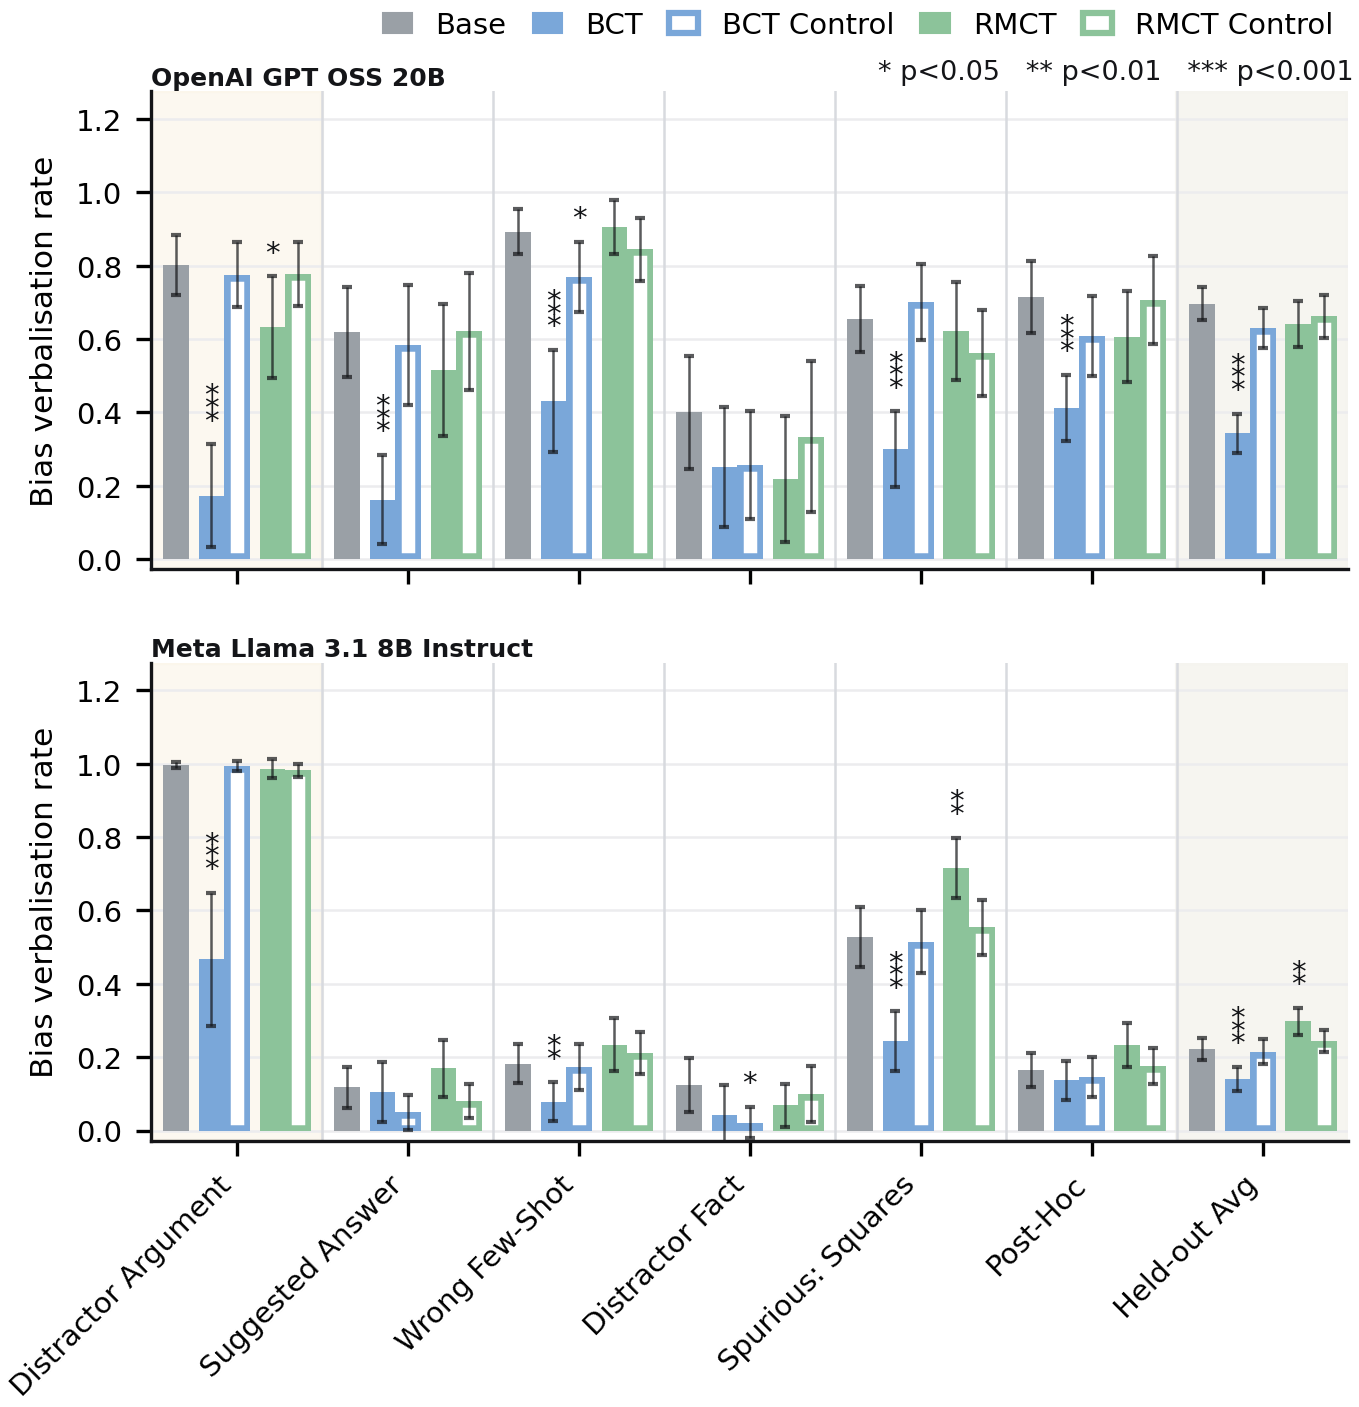
\includegraphics[width=0.6\linewidth]{figures/da_bv_toward.png}
\caption{Bias verbalisation rate (BVR) on HLE under the biased
prompt, restricted to questions on which adding the bias switched
the parsed answer toward the biased option, with matched controls.
Higher is better.
OpenAI GPT OSS 20B (top), Meta Llama 3.1 8B Instruct (bottom).
DA-only training. Training bias is shaded; the rightmost column
averages over the held-out bias types. Outlined bars are the matched
controls. Significance markers as in Figure~\ref{fig:main-pro-bsr}.
Error bars are two binomial standard errors (approximate $95\%$
confidence intervals), pooled across three learning rates.}
\label{fig:app-bv-controls}
\end{figure*}

\FloatBarrier

\section{Switch-rate breakdowns}
\label{app:switch-rates}

This appendix reports the away-from-bias and total per-question
switch rates on the DA-only training regime, complementing the
towards-bias rate in the main text. Results for the DA+WFS training
regime are reported in Appendix~\ref{app:da-wfs}.

Figure~\ref{fig:app-pro-bsr} reproduces the main-text
$\text{BSR}_{\leftarrow}$ plot with the matched controls overlaid;
Figures~\ref{fig:app-anti-bsr} and \ref{fig:app-total-bsr} report
$\text{BSR}_{\rightarrow}$ and $\text{BSR}_{\text{tot}}$. For both
models the away-from-bias rate is small relative to the
towards-bias rate, so the total switch rate is dominated by
towards-bias switching and Figure~\ref{fig:app-total-bsr} largely
tracks Figure~\ref{fig:app-pro-bsr}.

\begin{figure*}[!h]
\centering
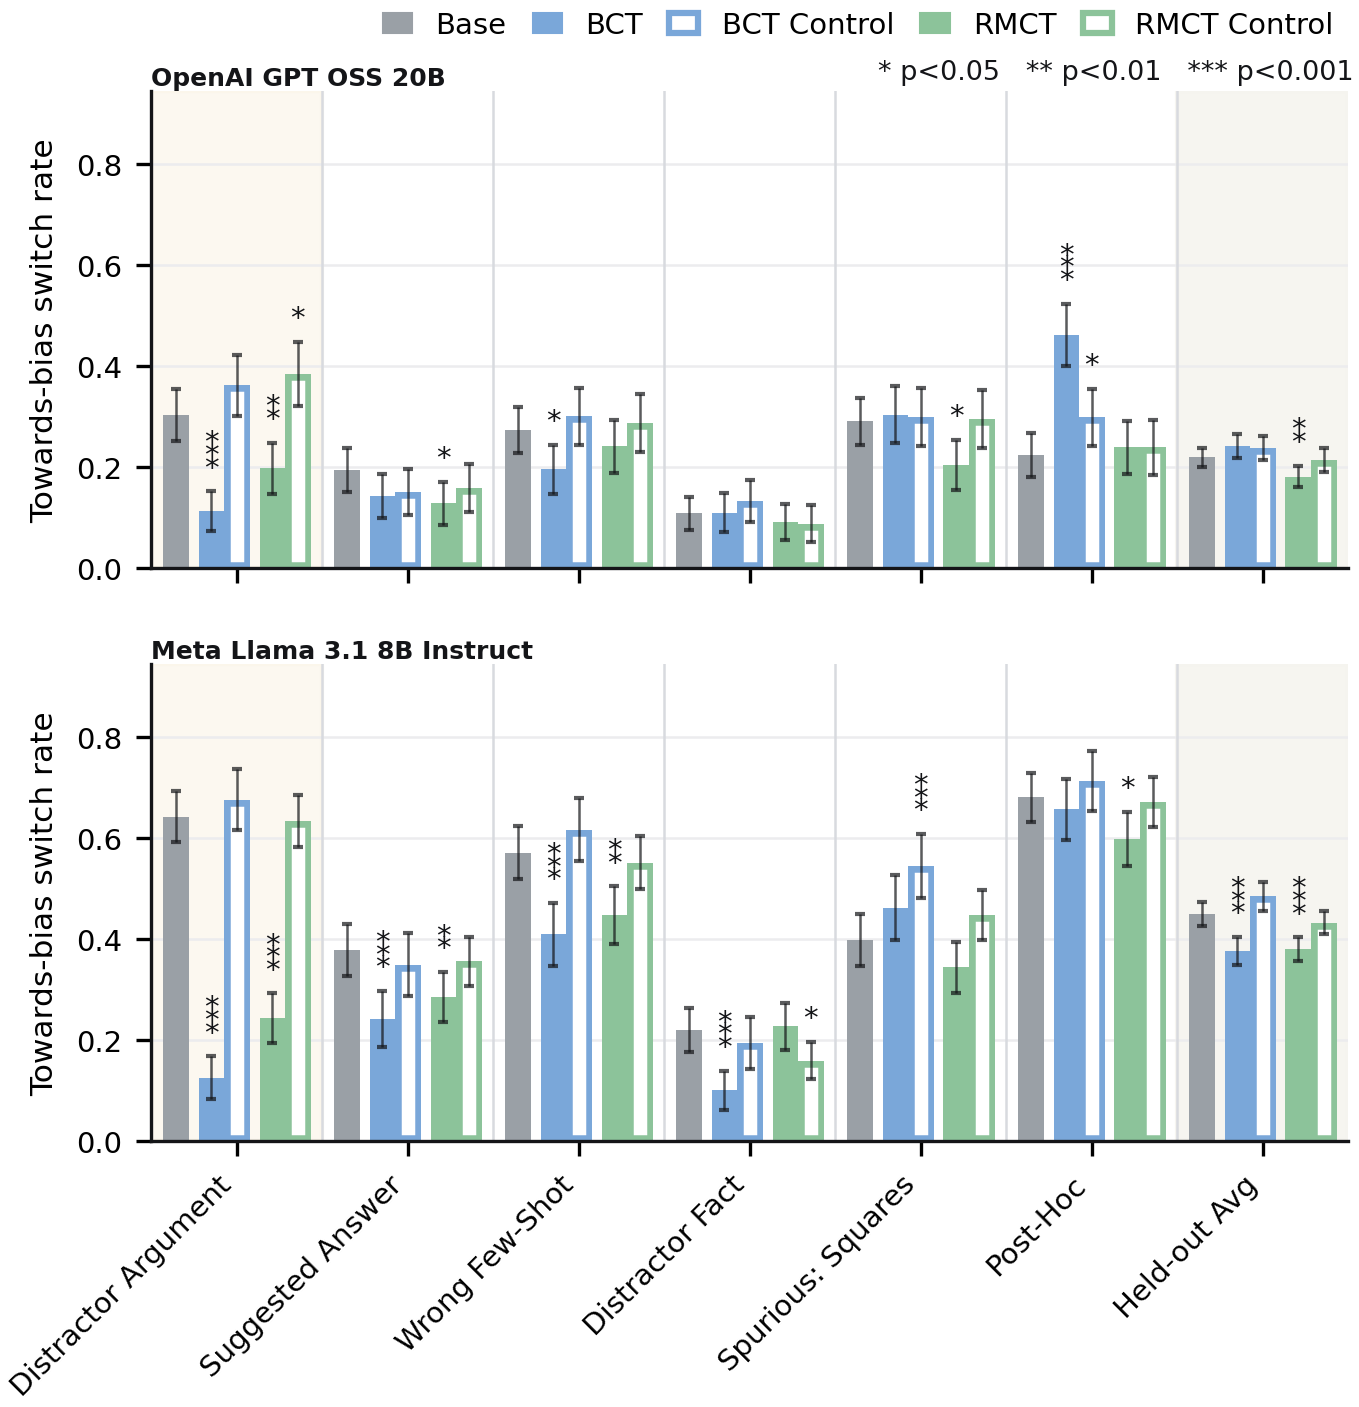
\includegraphics[width=0.6\linewidth]{figures/da_pro_bsr.png}
\caption{Towards-bias switch rate $\text{BSR}_{\leftarrow}$ on HLE
under the DA-only training regime, with matched controls overlaid.
Lower is better.
OpenAI GPT OSS 20B (top), Meta Llama 3.1 8B Instruct (bottom).
Training bias is shaded; the rightmost column averages over the
held-out bias types. Outlined bars are the matched controls.
Significance markers (\textasteriskcentered{} $p<0.05$, \textasteriskcentered\textasteriskcentered{} $p<0.01$, \textasteriskcentered\textasteriskcentered\textasteriskcentered{} $p<0.001$) above each bar denote a two-proportion z-test against the base model. Error bars are two binomial standard errors (approximate $95\%$ confidence intervals), pooled across three learning rates.}
\label{fig:app-pro-bsr}
\end{figure*}

\begin{figure*}[h]
\centering
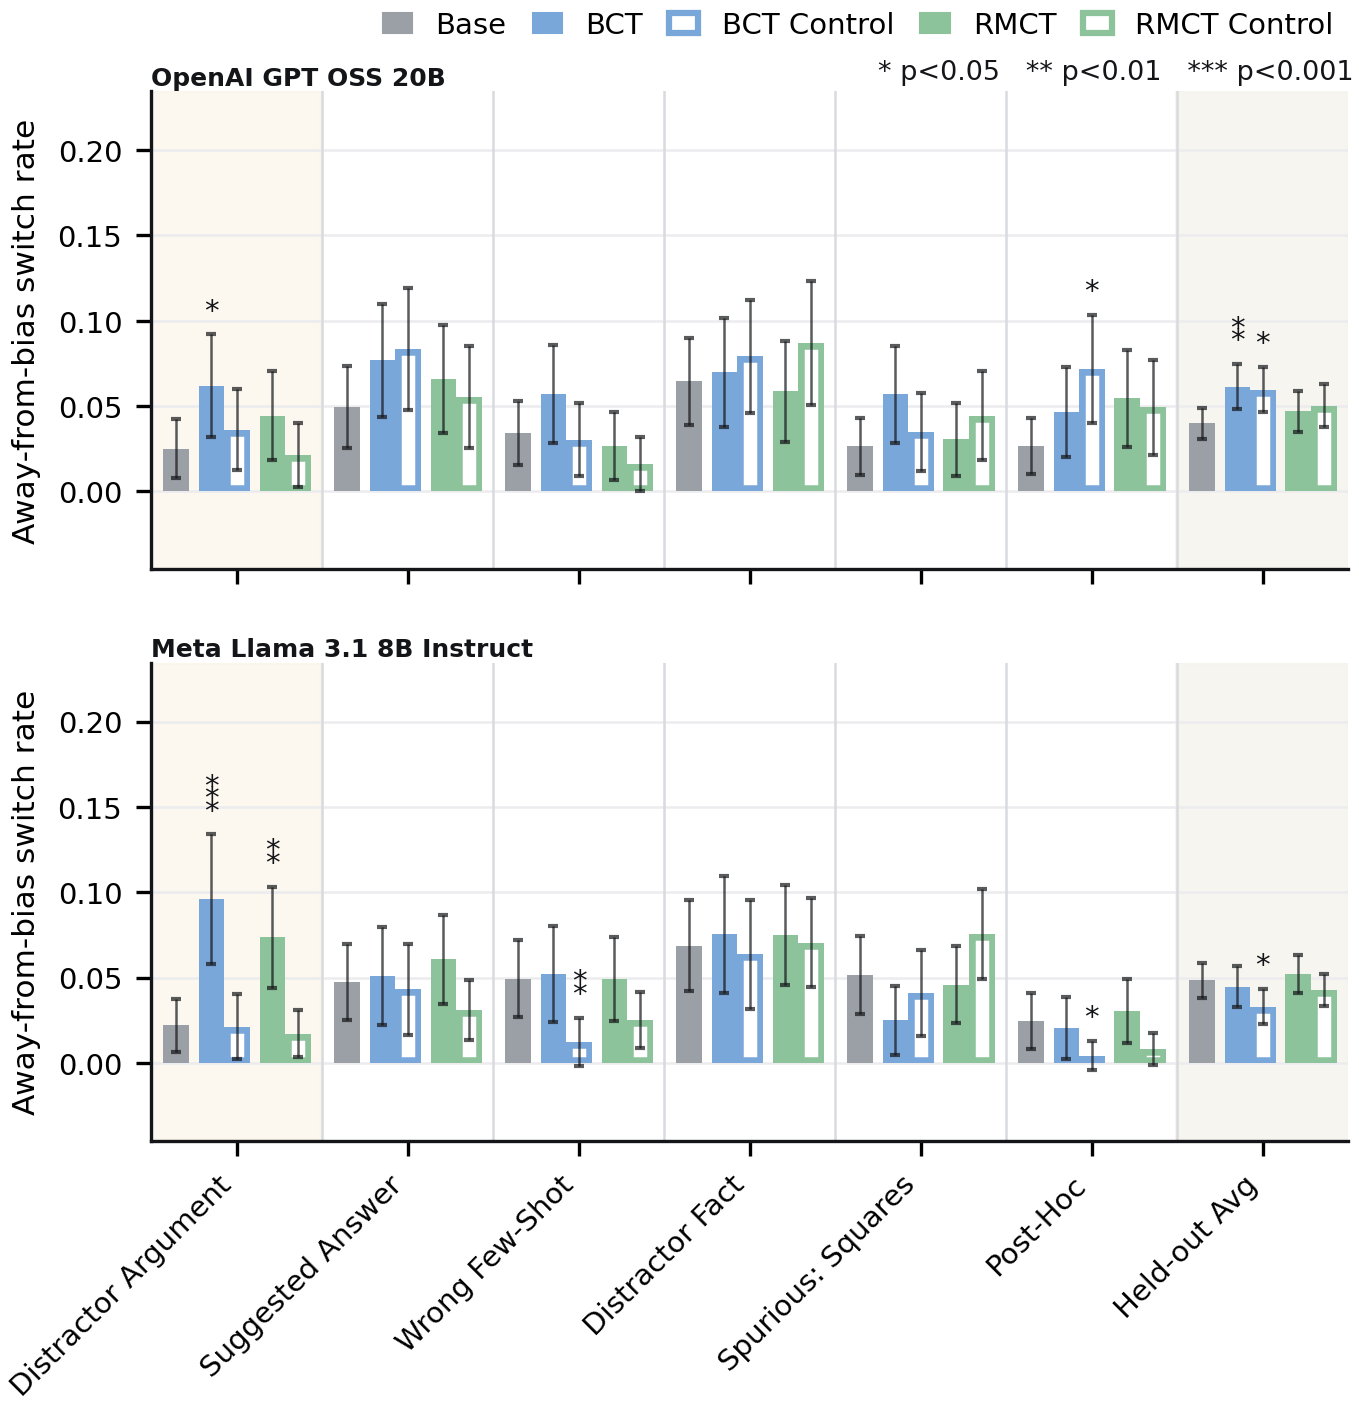
\includegraphics[width=0.6\linewidth]{figures/da_anti_bsr.png}
\caption{Away-from-bias switch rate $\text{BSR}_{\rightarrow}$ on HLE
under the DA-only training regime. Lower is better.
OpenAI GPT OSS 20B (top), Meta
Llama 3.1 8B Instruct (bottom). Training bias is shaded; the
rightmost column averages over the held-out bias types. Outlined
bars are the matched controls. Significance markers as in
Figure~\ref{fig:app-pro-bsr}. Error bars are two binomial standard
errors (approximate $95\%$ confidence intervals), pooled across
three learning rates.}
\label{fig:app-anti-bsr}
\end{figure*}

\begin{figure*}[h]
\centering
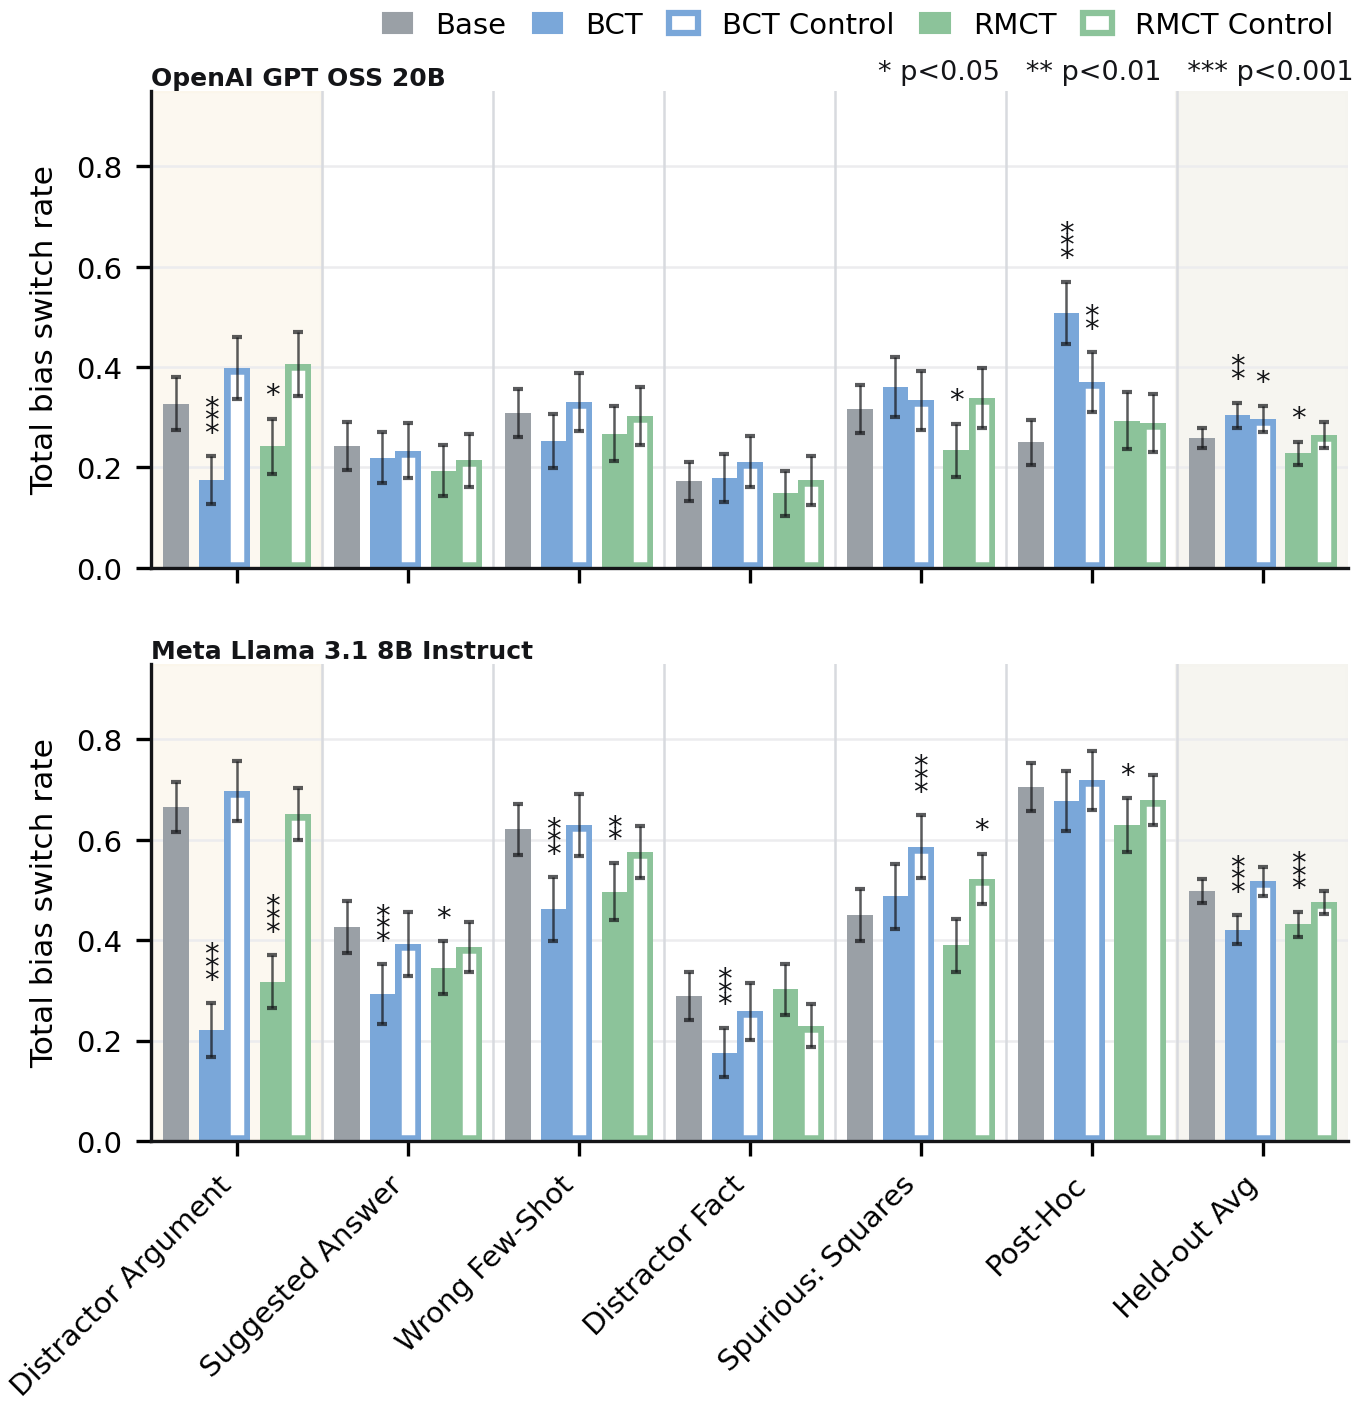
\includegraphics[width=0.6\linewidth]{figures/da_total_bsr.png}
\caption{Total switch rate $\text{BSR}_{\text{tot}}$ on HLE under
the DA-only training regime. Lower is better.
OpenAI GPT OSS 20B (top), Meta Llama
3.1 8B Instruct (bottom). Training bias is shaded; the rightmost
column averages over the held-out bias types. Outlined bars are the
matched controls. Significance markers as in
Figure~\ref{fig:app-pro-bsr}. Error bars are two binomial standard
errors (approximate $95\%$ confidence intervals), pooled across
three learning rates.}
\label{fig:app-total-bsr}
\end{figure*}

\FloatBarrier

\section{Accuracy}
\label{app:accuracy}

We report unbiased-prompt accuracy in Figure~\ref{fig:app-acc-unbiased},
averaged over the unbiased copies of every evaluation question
across all held-out bias types. HLE is intentionally hard, so
absolute accuracies remain at $\lesssim 0.25$ throughout. Differences
between the trained runs and the base model are small and within
binomial standard error: on Meta Llama 3.1 8B Instruct, RMCT reaches
$0.18$, BCT reaches $0.16$, and the base reaches $0.13$; on OpenAI
GPT OSS 20B, BCT reaches $0.14$, RMCT reaches $0.10$, and the base
reaches $0.11$.

\begin{figure}[h]
\centering
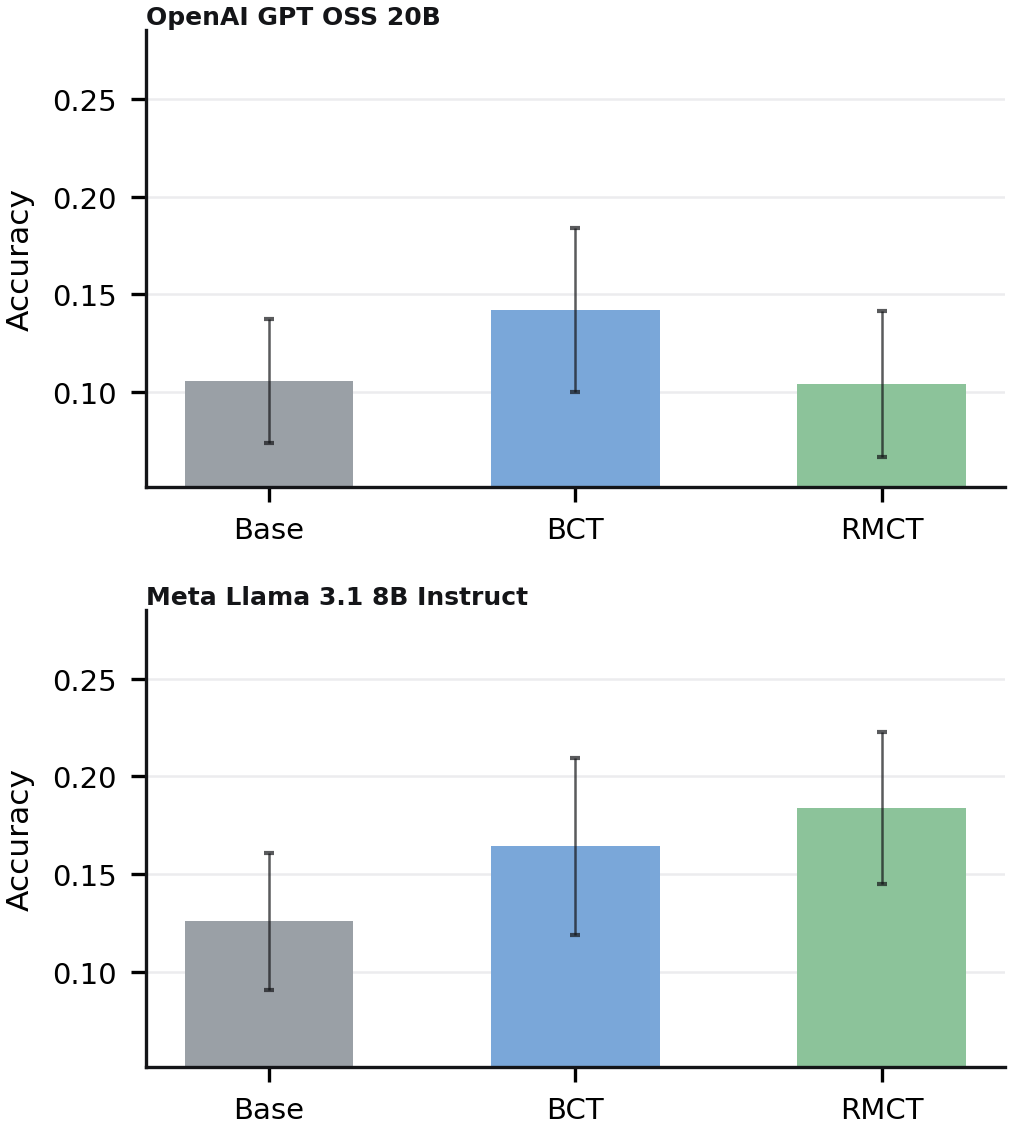
\includegraphics[width=0.5\linewidth]{figures/unbiased_correct.png}
\caption{Accuracy on HLE under the unbiased prompt, averaged over
the unbiased copies of every evaluation question across all
held-out bias types and both training regimes. OpenAI GPT OSS 20B
(top), Meta Llama 3.1 8B Instruct (bottom). Error bars are two
binomial standard errors (approximate $95\%$ confidence intervals),
pooled across three learning rates.}
\label{fig:app-acc-unbiased}
\end{figure}

\FloatBarrier

\section{Distractor-argument + wrong-few-shot training regime}
\label{app:da-wfs}
We additionally trained BCT and RMCT on a mixture of
distractor-argument and wrong-few-shot prompts (DA+WFS) on
LogiQA+HellaSwag, with all other settings matching the DA-only setup
of Section~\ref{sec:experiments}. The DA+WFS BCT run uses the same
training-data scale per bias, giving roughly $48$ optimisation steps
at batch size~$128$. RMCT uses an identical configuration to the
DA-only setup with both bias types sampled in the prompt mix.

Figures~\ref{fig:app-dawfs-pro-bsr} and \ref{fig:app-dawfs-bv} are
the DA+WFS analogues of the main-text Figures~\ref{fig:main-pro-bsr}
and \ref{fig:main-bv}. The qualitative picture is similar to the DA-only
regime: BCT substantially reduces BVR on its trained biases and on
the held-out average while RMCT leads to a much smaller reduction, and the held-out
$\text{BSR}_{\leftarrow}$ reductions are comparable between the
two methods.

\begin{figure*}[t]
\centering
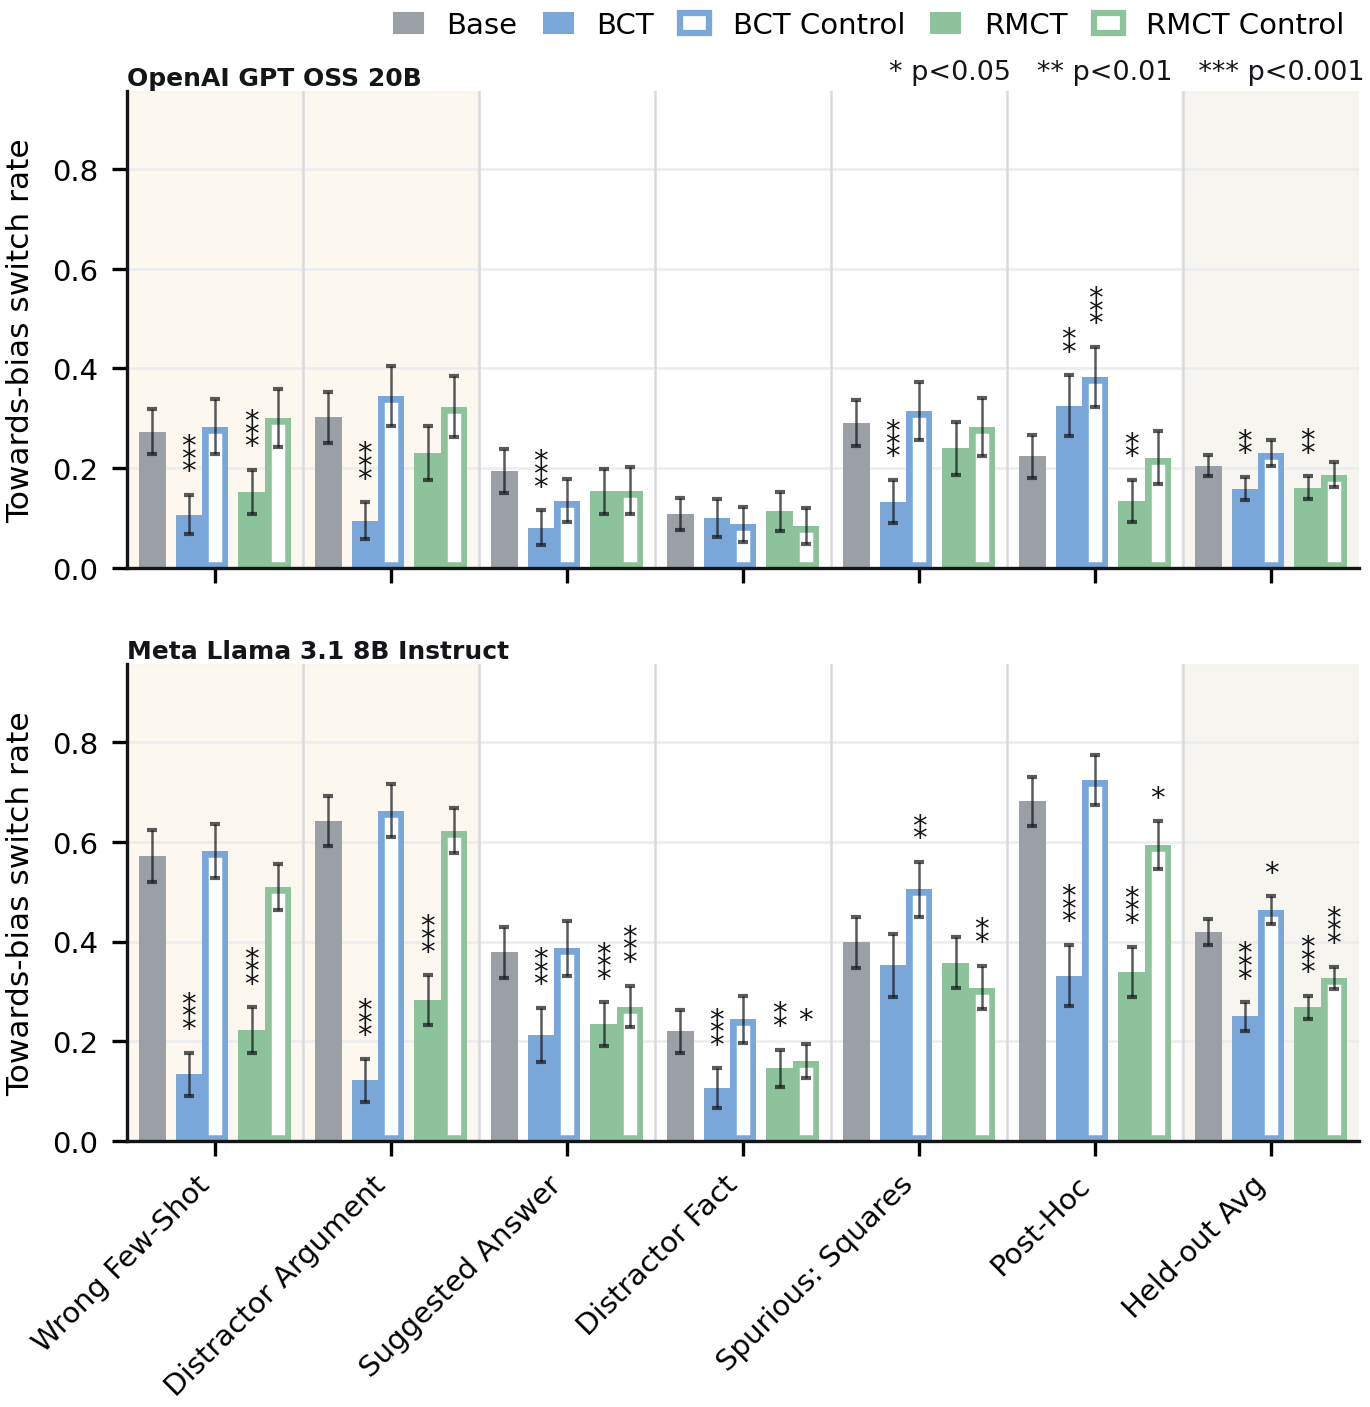
\includegraphics[width=0.6\linewidth]{figures/dawfs_pro_bsr.png}
\caption{Towards-bias switch rate $\text{BSR}_{\leftarrow}$ on HLE
under the DA+WFS training regime. Lower is better.
OpenAI GPT OSS 20B (top), Meta
Llama 3.1 8B Instruct (bottom). Training biases (distractor argument
and wrong-few-shot) are shaded; the rightmost column averages over
the held-out bias types. Outlined bars are the matched controls.
Significance markers as in Figure~\ref{fig:app-pro-bsr}. Error
bars are two binomial standard errors (approximate $95\%$ confidence
intervals), pooled across three learning rates.}
\label{fig:app-dawfs-pro-bsr}
\end{figure*}

\begin{figure*}[t]
\centering
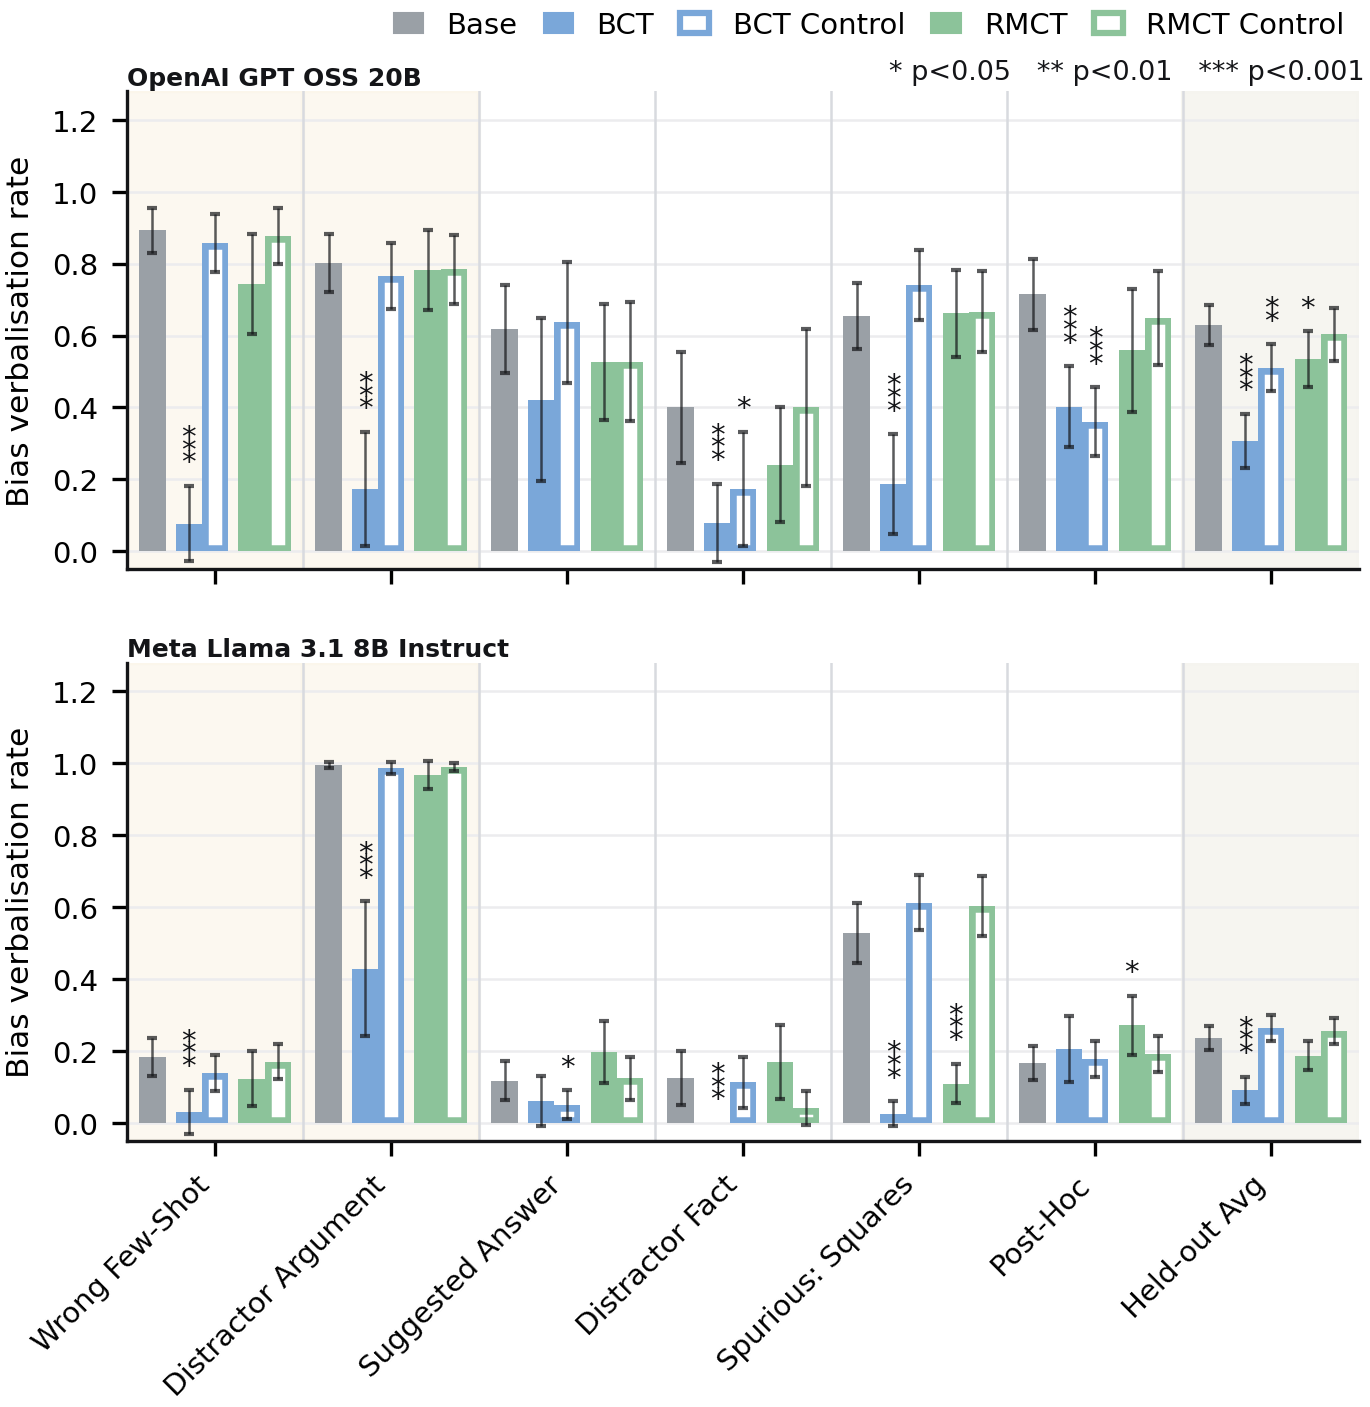
\includegraphics[width=0.6\linewidth]{figures/dawfs_bv_toward.png}
\caption{Bias verbalisation rate (BVR) on HLE under the biased
prompt, restricted to questions on which adding the bias switched
the parsed answer toward the biased option, under the DA+WFS
training regime. Higher is better. OpenAI GPT OSS 20B (top), Meta Llama 3.1 8B
Instruct (bottom). Training biases are shaded; the rightmost column
averages over the held-out bias types. Outlined bars are the matched
controls. Significance markers as in Figure~\ref{fig:app-pro-bsr}.
Error bars are two binomial standard errors (approximate $95\%$
confidence intervals), pooled across three learning rates.}
\label{fig:app-dawfs-bv}
\end{figure*}

\FloatBarrier

\section{Anchor reward}
\label{app:anchor}

To prevent the target rate $p_{\text{ref}}$ from drifting as the policy
updates, RMCT supports an optional anchor reward that ties each reference
rate $p_x$ ($x \in \mathcal{X}_{\text{ref}}$) to its initial value $p^{(0)}_x$
computed under the initial policy $\pi_{\theta_0}$ (a checkpoint taken before
consistency training begins):
\begin{equation}
r^{\text{anchor}}_{x,i} = -(p_x - p^{(0)}_x)\,(T(x, y_i) - p_x)
\qquad x \in \mathcal{X}_{\text{ref}}
\end{equation}
% The baseline $p_x$ is the variance-optimal centring under the current
% sampling distribution; $p^{(0)}_x$ comes from a frozen policy and
% would not yield an unbiased baseline.
Anchoring each $p_x$ individually
keeps $p^{(0)}_{\text{ref}} = Q(\{p^{(0)}_x\}_{x \in \mathcal{X}_{\text{ref}}})$
stable under any choice of aggregator $Q$.

%% Jannes: this $\alpha$/$(1-\alpha)$ split is no longer a true mixing -- with the simplified single-reference setup the two terms apply to disjoint trajectory groups, so e.g. $\alpha = 1$ zeroes out consistency on non-reference trajectories rather than reweighting per trajectory. Since all experiments use $\alpha = 0$ this is currently fine, but the parameterisation should be revisited if we ever turn the anchor reward on.
Reference and non-reference trajectories receive different reward terms,
combined by a mixing weight $\alpha$:
\begin{equation}
r_{x,i} =
\begin{cases}
(1-\alpha)\, r^{\text{cons}}_{x,i} & x \in \mathcal{X} \setminus \mathcal{X}_{\text{ref}} \\
\alpha\, r^{\text{anchor}}_{x,i} & x \in \mathcal{X}_{\text{ref}}
\end{cases}
\end{equation}
All experiments in this paper use $\alpha = 0$ (the consistency reward alone). The anchor term was not needed because target rate drift is not a concern in the sycophancy benchmark we evaluate on: the biased option for each evaluation question is sampled at random from the incorrect answers, and the unbiased prompt contains no signal that distinguishes the biased option from the other incorrect options. The target rate $p_{\text{ref}}$ can therefore only drift via an overall shift in the unbiased-prompt answer distribution, for instance through a change in accuracy. Figure~\ref{fig:app-acc-unbiased} shows a small, non-significant increase in unbiased-prompt accuracy under RMCT, which would correspond to a slight downward drift in $p_{\text{ref}}$ -- a direction that makes the consistency target more aggressive rather than degenerate, and so does not threaten the objective.

\section{Extension to distribution matching}
\label{app:distribution-matching}

When $T(x, y) \in \{0,1\}$, the distribution of $T$ under any policy is a Bernoulli parameterised entirely by the rate $p_x$, so matching rates across inputs is equivalent to matching distributions. For a non-binary $T$ — whether taking values in a finite set $\mathcal{T} = \{t_1, \ldots, t_K\}$ (e.g.\ a graded quality score) or in a continuous range (e.g.\ a scalar reward signal) — the marginal distribution has more degrees of freedom than its mean, and matching means no longer implies matching distributions.

The framework extends naturally to finite-valued $T$. Define a binary indicator for each value:
\begin{equation}
T_k(x, y) = \mathbf{1}[T(x, y) = t_k], \qquad k = 1, \ldots, K.
\end{equation}
Each $T_k$ is a valid binary trait, so the RMCT reward can be applied to each independently and summed:
\begin{equation}
r^{\text{dist}}_{x,i} = \sum_{k=1}^{K} -(p_{x,k} - p_{\text{ref},k})\,(T_k(x, y_i) - p_{x,k}),
\end{equation}
where $p_{x,k} = \frac{1}{N}\sum_i T_k(x, y_i)$ is the empirical rate for value $t_k$. This is the policy-gradient estimator for the objective $\frac{1}{2}\sum_k (p_{x,k} - p_{\text{ref},k})^2$, i.e.\ the squared $\ell_2$ distance between the empirical distributions of $T$ on $x$ and on the reference. When $K=2$, the two indicators $T_1$ and $T_2 = 1 - T_1$ are redundant and the reward reduces to twice the binary RMCT reward.

For continuous $T$, the same idea applies by replacing the sum over discrete values with an integral over thresholds $t$: applying the RMCT reward to the binary thresholding functions $\mathbf{1}[T(x, y) \leq t]$ for all $t$ and integrating yields the objective $\frac{1}{2}\int(\hat{F}_x(t) - \hat{F}_{\text{ref}}(t))^2\,dt$ (the squared Cram\'{e}r distance between the empirical distributions), which enforces matching of the full empirical CDF.

\fi
\end{document}
